% ------ METADATA ------
\newcommand{\bookauthor}{\ml{$0$}{Эмиль~Весна}{Emil~Viesn\'{a}}}
\newcommand{\booktitle}{\ml{$0$}{ЦВЕТЫ~ДЛЯ~БАБУШКИ}{Flowers~for~the~Old~Woman}}
\newcommand{\bookstarted}{\ml{$0$}{19 августа 2017}{August 19, 2017}}
\newcommand{\bookfinished}{\ml{$0$}{пока нет}{not yet}}
% ------ METADATA ------

% ----- XELATEX SYMBOL -----
\usepackage{xltxtra}
% ----- XELATEX SYMBOL -----

% ----- HYPHENATION -----
\usepackage{hyphenat}
% ----- HYPHENATION -----

% ----- GEOMETRY -----
\usepackage[left=1.5cm,right=1.5cm,top=2cm,bottom=2cm,bindingoffset=0.5cm]{geometry}
% ----- GEOMETRY -----

% ----- INCLUDE PDF AS PAGES -----
\usepackage{pdfpages}
% ----- INCLUDE PDF AS PAGES -----

% ----- TOC CONFIG -----
\setcounter{tocdepth}{0}
\usepackage{titletoc}
\titlecontents{chapter}[0pt]{\large}%above code
{\MakeUppercase{\chaptername~\thecontentslabel}. }
{}%numberless chapter%
{\mdseries\titlerule*[0.75em]{.}\thecontentspage}
% ----- TOC CONFIG -----

% ----- DROPPING CAP -----
\usepackage{type1cm,lettrine}
% ----- DROPPING CAP -----

% ----- FONTS -----
\renewcommand{\baselinestretch}{1.2}
\setmainfont{Linux Libertine}
% ----- FONTS -----

% ------ HYPERLINKS ------
\usepackage{hyperref}
\definecolor{LinkColor}{HTML}{0969DA}
\hypersetup{colorlinks=true, linkcolor=LinkColor, citecolor=LinkColor, filecolor=LinkColor, urlcolor=LinkColor}
% ------ HYPERLINKS ------

% ------ VKONTAKTE MESSAGES ------
\usepackage{changepage}
\definecolor{VkBlue}{HTML}{3F72B0}
\newfontfamily\vkfont{Roboto}
\newcommand{\VKmessage}[2]{\begin{adjustwidth}{1cm}{1cm}{\vkfont\footnotesize\textcolor{VkBlue}{\textbf{#1}}\\#2}\end{adjustwidth}\hspace{0.1em}}
% ------ VKONTAKTE MESSAGES ------

% ----- OLD TYPING -----
\newfontfamily\oldfont{TrixieCyr-Pre2}
\newcommand{\oldtyping}[1]{{\hspace{0.1em}\oldfont\small{#1}\par}\hspace{0.1em}}
% ----- OLD TYPING -----

% ----- CODE -----
\newfontfamily\codefont{Hack}
\newcommand{\somecode}[1]{{\codefont{\textbf{\small{#1}}}}}
% ----- CODE -----

% ------ FANCY PAGE STYLE ------
\setlength{\headheight}{15pt}
\usepackage{fancyhdr}
\pagestyle{fancy}
\fancyhead[LE,RO]{\thepage}
\fancyhead[LO]{{\small\textsc{\booktitle}}}
\fancyhead[RE]{{\small\textsc{\bookauthor}}}
\fancyfoot{}
    \fancypagestyle{plain}{
    \renewcommand{\headrulewidth}{0mm}
    \fancyhead{}
    \fancyfoot{}
}
% ------ FANCY PAGE STYLE ------

% ------ ELEMENTS ------
\newcommand{\asterism}{\vspace{1em}{\centering\Large\bfseries$\ast~\ast~\ast$\par}\vspace{1em}}
\newcommand{\textspace}{\vspace{1em}{\centering\Large\bfseries<\dots>\par}\vspace{1em}}
\newcommand{\FM}{\footnotemark}
\newcommand{\FA}[1]{\footnotetext{#1 \emph{\ml{$0$}{---~Прим.~авт.}{---~Author.}}}}
% ------ ELEMENTS ------

% ------ NAMES ------
\newcommand{\Angstrem}{Angstr\'em}
\newcommand{\gopnik}{g\'opnik}
\newcommand{\Ilgiza}{Ilgiz\'a}
\newcommand{\Izolda}{Iz\'olda}
\newcommand{\Kalgin}{Kalg\'{\i}n}
\newcommand{\Kirya}{K\'{\i}rya}
\newcommand{\Koltsovo}{Kolts\'ovo}
\newcommand{\MaksimOrlov}{Maks\'{\i}m Orl\'ov}
\newcommand{\militsioner}{militsion\'er}
\newcommand{\militsiya}{mil\'{\i}tsiya}
\newcommand{\Nikolay}{Nikol\'ay}
\newcommand{\Ondar}{Ond\'ar}
\newcommand{\Preobrazhenskaya}{Preobrazh\'enskaya}
\newcommand{\Rita}{R\'{\i}ta}
\newcommand{\Sasha}{S\'asha}
\newcommand{\Shenkerman}{Shenkerm\'an}
\newcommand{\Shishkin}{Sh\'{\i}shkin}
\newcommand{\silovik}{silov\'{\i}k}
\newcommand{\tovarisch}{tov\'arisch}
\newcommand{\Valera}{Val\'era}
\newcommand{\Varenik}{Var\'enik}
\newcommand{\Varyonych}{Vary\'onych}
\newcommand{\Veronika}{Veron\'{\i}ka}
\newcommand{\Vladimir}{Vlad\'{\i}mir}
\newcommand{\Vladimirovich}{Vlad\'{\i}mirovich}
\newcommand{\Vladislavovna}{Vladisl\'avovna}
\newcommand{\Volodka}{Vol\'odka}
\newcommand{\Volod}{Vol\'od}
\newcommand{\Volodya}{Vol\'odya}
\newcommand{\Volya}{V\'olya}
\newcommand{\Yasha}{Y\'asha}
\newcommand{\Yelena}{Yel\'ena}
\newcommand{\Zhenya}{Zh\'enya}
% ------ NAMES ------

\begin{document}

% ----- FRONT COVER -----
\includepdf[pages={1}]{\coverfrontfilename}
% ----- FRONT COVER -----

% ----- EMPTY PAGE -----
\newpage\thispagestyle{plain}~
% ----- EMPTY PAGE -----

% ------ TITLE PAGE ------
\begin{titlepage}
{
\centering
{~\par}
\vspace{0.25\textheight}
{\LARGE\bookauthor\par}
\vspace{1.3cm}
{\Huge\textbf{\booktitle}\par}
\vfill
{\includegraphics[width=6em]{\publisherlogofilename}\par}
}
\end{titlepage}
% ------ TITLE PAGE ------

% ----- TRIGGER WARNING -----
\newpage\thispagestyle{plain}
{~\par}
\vfill
{\centering
\includegraphics[width=4em]{tw.pdf}\par}
\vspace{1em}
{\centering\Large\strong{\ml{$0$}{Предупреждение}{Content Warning}}\par}
\vspace{0.5em}
{\centering\large{Данное произведение содержит описание неизлечимых болезней, психических состояний, врачебных манипуляций, упоминания суицида, химических зависимостей, сцены насилия и убийств, мат, а также гомофобную, трансфобную, сексистскую и расистскую лексику.}\par}
\vfill
{~\par}
% ----- TRIGGER WARNING -----

% ----- TABLE OF CONTENTS -----
\tableofcontents
% ----- TABLE OF CONTENTS -----

% ----- DISCLAIMER PAGE -----
\newpage\thispagestyle{plain}
{~\par}
\vfill
{\centering\Large\textit{
\ml{$0$}
{Светлой памяти Риты "---\\девочки, которая принимала роды у козы\\и которая кормила меня кексами\\в худшие дни моей жизни.}
{To the loving memory of \Rita,\\the girl who delivered a goatling\\and who fed me muffins\\on my worst days.}
}\par}
\vfill
{~\par}
% ----- DISCLAIMER PAGE -----

\pagestyle{fancy}

\chapter{\ml{$0$}{Отголосок бури}{The Echo of the Storm}}

\label{Mon_2012_04_09}

\lettrine[lines=4,slope=0pt,nindent=3pt]{В}{спомните} свой самый худший кошмар.
Вспомнили?
Во всех подробностях?
Отлично.
Я не знаю, что вы увидели, но могу вас уверить: это ерунда по сравнению с царём кошмаров.

Самый худший кошмар на свете выглядит достаточно безобидно.
Кошмар ограниченного мира.
Вариаций может быть огромное множество, и Варенику сегодня приснилась одна из них.
Звёздное небо, дом с пустыми окнами, занесённый тонким слоем снега переулок и пять могил на обочине.

Важная часть кошмара ограниченного мира "--- осознанность и кратковременная иллюзия всемогущества.
Да, я во сне, а значит, всё, что я могу придумать, может стать реальностью!
И только взлетев, распахнув крылья, ощутив биение воздуха в грудь, Вареник понял "--- не может.

Далёкие звёзды оказались простыми источниками света, подвешенными в пустоте.
Дом превратился в картонку с прорезями, а переулок "--- в единственное во всей этой карманной Вселенной место, где можно стоять и существовать.

Больше там ничего не было.

Вареник спустился к могилам и начал читать надгробия:

\begin{quote}
Шенкерман Владимир Владимирович (1986--2048)

Сафронова"--~Зима Вероника Андреевна (1989--2072)

Лебедев Сергей Валерьевич (2010--2045)

Колесникова Маргарита Михайловна (2005--2090)
\end{quote}

Последняя могила, принадлежащая <<Сафронову Валерию Николаевичу (1985--2028)>>, была пустой.
Кто-то положил на дно клетчатое одеяло, приглашающе отогнув уголок.

Что, если бы вы не смогли проснуться?

Варенику повезло "--- он проснулся.
Могилы и снег сменились теплом постели и живой, невероятно живой жены с огненно-рыжими волосами.
И даже мысль о сходстве карманной и реальной Вселенной его не посетила.
Ему вообще везло "--- и с мыслями, и с женой, и с самой жизнью, "--- как и семи миллиардам смертных, которым есть куда проснуться и есть куда умереть.

Впрочем, именно сегодня он не чувствовал себя везучим.
На утро было назначено очередное собеседование.

\asterism

\ml{$0$}
{"--*Извините, вы нам не подходите.}
{``I'm afraid you're not right for the job.''}

Стандартная фраза.
Вареник слышал её уже в одиннадцатый раз.
Говорили на собеседованиях разное, но слышал он одно и то же.
Иногда проводивший собеседование эйчар даже начинал извиваться и кривиться, словно змея на сковороде;
Вареник знал "--- наступил момент, когда уже всё ясно, деньги отработаны, а желудок требует заслуженной чашки корпоративного кофе.

"--*Счастливо, "--- коротко ответил Вареник и, собрав свои бумаги, вышел из кабинета.

В этом офисе, как и в прочих других, царил декаданс.
Современные материалы, на поверку оказывающиеся отходами производства.
Запах парфюмерии, сквозь который пробивались ароматы непролеченных язв и убитых алкоголем почек.
Десятки людей с агрессивно-равнодушными взглядами, прячущими страх безработицы, ощущение собственной незначительности и два-три непогашенных кредита.

<<Может, оно и к лучшему>>, "--- решил про себя Вареник, ощущая тяжёлый взгляд охранника.
Тот крутил на пальце ключи.
Две тысячи лет назад жил человек, который с точно таким же выражением лица поигрывал кнутом.
Этого не было ни в одной хронике, ни в одном учебнике, но Вареник знал это так, словно видел своими глазами.

<<Прости, Вероника.
Хуёвый у тебя муж>>.

\asterism

Предчувствие очередной неудачи преследовало Вареника с утра "--- с того самого момента, как он покинул мир с пятью могилами.

Вначале он вспомнил, что его рабочая лошадка, Тойота Королла две тысячи второго года выпуска, стоит в автосервисе, и ехать придётся общественным транспортом.
Затем выяснилось, что интернет закончился в полночь, и узнать дорогу к офису компании можно только у точки бесплатного вайфая в двух остановках от дома.
Наконец, уже настроившись перехватить в кафе пирожок, он выяснил, что забыл в другой куртке карту.
Налички было впритык на дорогу.

Офис находился на возвышенности;
ледяной ветер с Оби забирался под куртку и сбивал с ног.

Охрана сразу встретила его неприветливо.

\ml{$0$}
{"--*Я на собеседование.}
{``I'm here for my job interview.''}

\ml{$0$}
{"--*К кому?}
{``Who invited you?''}

\ml{$0$}
{<<В смысле "--- к кому?>>}
{\textit{What do you mean, ``who''?}}
\ml{$0$}
{В здании находилась только одна компания.}
{There was only one company in the building.}

\ml{$0$}
{"--*Щас.}
{``Wait a sec.''}

Вареник выудил телефон и начал искать СМС с данными компании.

\ml{$0$}
{"--*Фома Непомнящий, блядь, "--- плюнул охранник.}
{``Doubting fucking Thomas,'' the guard spitted.}
\ml{$0$}
{"--- Идёт, а к кому "--- не помнит.}
{``En route to who-knows-who.''}

\ml{$0$}
{"--*Максим Орлов, "--- сказал Вареник, проигнорировав реплику.}
{``\MaksimOrlov.'' \Varenik\ ignored the guard's words.}

\ml{$0$}
{"--*Ну так и звоните ему.}
{``Call him on the phone.''}

\ml{$0$}
{"--*До собеседования ещё час, "--- сказал Вареник.}
{``I have an hour before the interview,'' \Varenik\ said.}
\ml{$0$}
{"--- На улице ветрено, и я думал, просто посижу здесь.}
{``It's windy outside, I hoped I'll just sit here.''}

\ml{$0$}
{"--*Здесь вы не посидите, "--- обрадовал его охранник.}
{``You won't just sit here.'' The guard was definitely trying to make him happy.}
\ml{$0$}
{"--- Приходите ко времени.}
{``Come as scheduled.''}

Вареник кивнул и направился к выходу.
В обычной ситуации он бы мысленно или вслух выругался, но это было его одиннадцатое собеседование, и тратить силы на очередного чоповца с синдромом вахтёра не хотелось.

Райончик оказался так себе.
Автострада, автомойки, автосервисы, несколько клиник, пара задрипанных ювелирных салонов и билборд <<Откажись от наркотиков!>>.
Как известно, билборды и надписи на стенах всегда соответствуют местному контингенту.
Ни одного кафе в радиусе километра.

Местный продуктовый был на три четверти заставлен спиртным, одну восьмую прилавков занимали семечки "--- ещё один намёк на местный контингент.
Собственно съестное робко ютилось в уголке.
Вареник купил крохотную пачку вафель, чтобы хоть как-то заполнить пустоту в желудке.
В жертву пошли деньги на маршрутку "--- придётся ждать автобуса.

Оставшиеся десять минут он провёл в странно современном цветочном магазине, чихая и делая вид, что рассматривает цветы.
Симпатичная продавщица на каждый чих говорила <<Будьте здоровы>> и понимающе вздыхала.

Всё это было зря.

\asterism

Выйдя из офисного здания, Вареник направился к метро.

К станции удалось выйти не сразу.
Дорожная развязка сыграла с пешеходом несколько ей одной понятных шуток, прежде чем милостиво вывела его на нужную улицу.
Вареник обрадовался и рванул через дворы, но радость оказалась преждевременной.
На пути встали несколько новостроек, окружённых глухими заборами;
шлагбаумы стояли, точно крохотные ландскнехты с огромными двуручными мечами.

<<Да какого хрена! "--- возмутился Вареник.
"--- Как вообще здесь выживать без автомобиля?!
Лабиринт ёбаный\ldots{}>>

Совсем некстати опять всплыл в памяти утренний сон.

Вареник ненавидел колючую проволоку и заборы с острыми пиками.
Эти вещи "--- не просто архитектурные ухищрения, не просто предупреждение;
это настоящее варварство, полное презрение к человеческим страданиям.
Ни одна страна не будет свободной, пока на её территории есть колючая проволока.
В России же даже в городах, предназначенных для проживания свободных людей, каждый второй дом, каждый промышленный или торговый объект ощерились острым металлом, словно зоны.
Пожалуй, единственное, что не имеет границ в России "--- стремление возводить границы.

"--*Э, куда полез, блядь! "--- заорал кто-то вдалеке, выбежав из маленькой будки.
Вареник аккуратно перемахнул через шипастое навершие забора, пропустив реплику мимо ушей.

Законы, финансы, политика, закрытые города, военные части, частная собственность "--- удавки, наброшенные на шею и не дающие сделать вдох ни на миллилитр больше, чем нужно для твоего выживания.
Живи, работай и даже не помышляй выйти за рамки.
И не думай, что эти рамки иллюзорны "--- нужно большое мужество, чтобы уйти за границы собственных финансов или привычек.

Большая часть России "--- дикая пустошь.
Но ты не можешь построить дом там, где хочешь, ты не можешь выращивать культуры и питаться от земли там, где хочешь.
Ты не можешь даже перемещаться по стране, не имея целой кипы бумаг "--- документов или валюты.

С деньгами всё становится проще.
Здоровая пища, лучшие врачи, любые удовольствия.
Ты можешь выбрать любое жильё "--- домик у моря, дворец во Франции или комната в коммуналке.
Ты можешь работать на любой работе, потому что тебе это нравится.
Ты можешь примерить на себя любую роль "--- пожарника, спасающего жизни, работяги с толстой женой, прожигающего жизнь мажора, измождённого шахтёра, мужчины по вызову, бездомного монаха в далёкой Индии.
Ты можешь поменять роль в любой момент, когда она тебе надоест.
Со стабильным источником больших денег выживание превращается в игру.

Без денег в этом мире ты просто раб, не имеющий права ни на что.

Вареник желал другого мира.
Но мир только один, что бы ни говорили на этот счёт теории мультивселенных.

\ldots{}Из-за домов выглянул кусочек оживлённой дороги, а затем показалась и большая красная буква \textbf{М}.
Философия вылетела из головы Вареника так же быстро, как и появилась.

\asterism

"--*Не взяли, "--- утвердительно сказала Вероника, едва лицо мужа показалось из-за двери.
"--- Иди кушать, через десять минут готово будет.

Вареник повиновался.
Он долго пытался влезть в плисовые штаны и слишком долго рассматривал комично-страшные морды тапочек-драконов.
Подарок Вероники.

"--*На, ешь, "--- Вероника поставила перед мужем тарелку с овощным супом.
\ml{$0$}
{"--- Ты очень грустный.}
{``You look very sad.}
\ml{$0$}
{Тебя обидел кто-то?}
{Did someone hurt you?''}

"--*Да нет, "--- буркнул Вареник.
"--- Просто долго что-то без работы сижу.
И подработок, как назло, нет "--- даже грузчики не нужны\ldots{}

Суп сделал Вареника чуть более разговорчивым.

"--*\ldots{}Понимаешь, я всё делаю по правилам! "--- говорил Вареник.
"--- Я выучил все эти стандартные вопросы-ответы на собеседованиях, проговорил, отработал!

\ml{$0$}
{"--*Верю, "--- кивнула Вероника.}
{``I believe,'' \Veronika\ nodded.}
\ml{$0$}
{"--- Только вот\ldots{}}
{``Just \ldots{}''}

\ml{$0$}
{Она вдруг заулыбалась.}
{She smiled.}

"--*Ну чего? "--- обиделся Вареник.

\ml{$0$}
{"--*Да хреновый из тебя врун, зай, "--- объяснила жена.}
{``You're a shit of a liar, hon,'' the wife explained.}
"--- Когда ты врёшь, тебя аж перекашивает всего, как будто тебе нанесли смертельную обиду.

"--*А, так вот как ты научилась различать, "--- буркнул Вареник.
"--- Видимо, мне капец.

Вероника нахмурилась и пристально вгляделась в мужа.

"--*Ты боишься, что я от тебя уйду?

"--*Нет, конечно, "--- Вареник улыбнулся, но голос его выдал.

Вероника вздохнула.

\ml{$0$}
{"--*Солнце, я знаю, что ты не лентяй.}
{``Sun, I know you're not lazy.}
\ml{$0$}
{Это временные трудности.}
{This is all just temporary.''}

\ml{$0$}
{"--*Да какие-то слишком временные.}
{``Too temporary, I'd say.''}

"--*Когда я в аварию попала, там вообще трудностям конца-края не было.
Мы это пережили.
Ты меня с ложки кормил, помнишь?

\ml{$0$}
{"--*Дело давнее.}
{``Bygones.''}

\ml{$0$}
{"--*Именно.}
{``Exactly.}
\ml{$0$}
{Всё это позади.}
{Bygones.}
\ml{$0$}
{А сейчас трудности у тебя.}
{Now it's you who's in trouble.}
\ml{$0$}
{И я буду рядом.}
{And I'm gonna be by your side.''}

Вероника набрала ложку супа и аккуратно поднесла её ко рту мужа.
Вареник усмехнулся и съел предложенное.
По пищеводу прокатилась волна живительного тепла.

\ml{$0$}
{"--*Я в тебе засомневался.}
{``I doubted you.}
\ml{$0$}
{Прости.}
{Sorry.}
\ml{$0$}
{Ты обиделась?}
{You feel offended?''}

\ml{$0$}
{"--*Нет.}
{``No.}
\ml{$0$}
{Я знаю, каково чувствовать себя беспомощной.}
{I understand what it's like to feel helpless.}
\ml{$0$}
{Засомневаешься в ком угодно.}
{You would doubt anyone.}
\ml{$0$}
{Тогда, в больнице\ldots{} я каждый день боялась, что тебя не дождусь.}
{That time, in the hospital \ldots{} every single day, I was afraid I wouldn't see you again.}
\ml{$0$}
{Что ты умрёшь, встретишь другую женщину, просто решишь, что я тебе надоела.}
{I was afraid you would die, or meet another woman, or just get tired of me.}
\ml{$0$}
{Что я просто останусь одна.}
{I was afraid I would be alone.}
Или, ещё хуже, ко мне начнёт ходить мать со своими вечными разговорами.
\ml{$0$}
{Она грозилась приехать и тебя отвадить, типа, ты уже труп, о душе думать надо, а он тебе голову любовью морочит\ldots{}}
{She threatened to come and ward you off, like, you're already dead, think of your soul, he's just fooling you with love \ldots{}''}

"--*Если бы ты мне об этом сказала, я бы её в труп превратил\ldots{}

"--*Да потому и не сказала!
Эта рухлядь и так нам достаточно проблем устроила.

"--*Что-то нам обоим не повезло с родителями, "--- заметил Вареник.

Поев, Вареник повеселел.
Да, безработность "--- это неприятно, но, к его счастью, кризис среднего возраста ему пока не грозил.

Вареник примерно понимал, откуда растут ноги у кризиса среднего возраста.
Всю молодость люди ставят себе какие-то цели.
Школьники должны закончить школу.
Студенты "--- выпуститься из универа.
Дипломированные молодые специалисты "--- найти тёпленькое местечко по специальности.
Холостые должны жениться, а бездетные "--- завести ребёнка.
И вот, когда все цели достигнуты, в голове человека возникает закономерный вопрос "--- а что, собственно, дальше?
Этот вопрос, как контрольный выстрел, добивает окончательно человеческую психику, и без того расшатанную школьными порядками, бессонными ночами перед сессией, орущим дитём и бесконечной <<работой над отношениями>>.

Отчасти Вареник даже был благодарен судьбе, что его <<победный марш>> оборвался на стадии поступления в универ.
Политех на два года получил хорошего человека, а хороший человек сохранил себе нервы.
Могло быть и хуже.

\asterism

Едва Вареник успел заварить чай, как зазвонил телефон.

"--*Варёныч, хай.
\ml{$0$}
{Как здравие?}
{How you feeling?''}

\ml{$0$}
{"--*Жив, Киря, твоими молитвами, "--- лаконично ответил Вареник.}
{``Alive, \Kirya, with the help of your prayers,'' \Varenik\ answered.}
\ml{$0$}
{"--- Сам как?}
{``You?''}

\ml{$0$}
{"--*Да как-то вот, Варёныч.}
{``Kind of sucks, \Varyonych.}
\ml{$0$}
{Короче, ушёл я из <<Ангстрема>>, и Воля ушёл.}
{In short, I retired from \Angstrem, and \Volya\ too.}
\ml{$0$}
{По твоим стопам.}
{Following in your footsteps.''}

Голос Кири выдавал его напряжение.

\ml{$0$}
{"--*Если ты хочешь занять, не могу помочь, "--- предупредил Вареник очевидный вопрос.}
{``If you need money, can't help,'' \Varenik\ prevented obvious question.}
"--- Я как уволился, так и без работы сижу.

\ml{$0$}
{"--*Бля, братан, "--- опечалился Киря.}
{``Sucks, bro,'' \Kirya\ sadly said.}
"--- Мож варик какой есть, чтоб по-быстрому?
Лавэ горит, Катька свалить грозится.
Я по кентам посмотрел "--- нихуя, у всех напряг.

"--*Напиши мне ВКонтакте, я тебе скину кое-что, "--- задумался Вареник.
"--- Вахтовая работа где-то за Уралом, я такую точно не потяну по здоровью.
Платят немного, но зато вагончик и жратва включены, с голоду не помрёшь.

\ml{$0$}
{"--*Заебись!}
{``Fuck yeah!}
Я тебе прям щас маякну!
От души, Варёныч!

"--*Говно вопрос, обращайся.

"--*Это с твоего склада? "--- поинтересовалась Вероника.

"--*Ага, "--- кивнул Вареник.
\ml{$0$}
{"--- Там походу всё.}
{``Looks like they're done.''}

\asterism

Торговая компания <<Ангстрем>> владела складами в нескольких регионах.
Ходили слухи, что её хозяин давно уже перешёл на более выгодный бизнес, перекупив часть акций известных торговых сетей;
склады остались придатком "--- малоприбыльным и морально устаревшим.

\ml{$0$}
{"--*КОООСТЯ, БЛЯЯЯ!}
{``K\'OSTYA, MOTHERFUCKER!}
\ml{$0$}
{Опять ты мне, сука, собрал бочку с порохом! "--- с этого крика кладовщика Жени начинался рабочий день Вареника.}
{You made a bloody gunpowder barrel, again!'' Every \Varenik's day on the job started with that shout of storekeeper \Zhenya.}

Уже слегка поддатый Костя бормотал извинения и шёл исправлять косяки в сборке.
Ещё совсем нестарый мужик бухал как чёрт две трети жизни.
\ml{$0$}
{Костю увольняли три раза, и три раза он возвращался "--- идти ему было некуда, и заменить его было некем.}
{K\'ostya was fired three times, and came back three times---he has nowhere to go, and there was no one to replace him.}

Киря же, в отличие от Кости, не косячил никогда.
Он кабанчиком метался по складу, молниеносно раскидывая брикеты и связки по коробам.

\ml{$0$}
{"--*Ну а хуле, "--- говорил Киря прочим, "--- хочешь жить "--- умей вертеться.}
{``Dafuck'', \Kirya\ used to say to others, ``you wanna live, you gotta spin.''}

\ml{$0$}
{Киря замечательно умел вертеться.}
{\Kirya\ was good at spinning.}
Он получал самую большую зарплату для его должности, его регулярно объявляли работником месяца и выдавали поощрения.
Он имел безусловный авторитет среди мужиков благодаря надёжности и честности.
Работа на складе была его коньком, а должность комплектовщика <<Ангстрема>> "--- венцом карьеры.

\ml{$0$}
{Вареник не хотел вертеться "--- он хотел жить.}
{\Varenik\ never wanted to spin, he wanted to live.}
Посему же ничем не выделялся среди других.
Ему нравился запах коробок и хруст, с которым они разрывались.
Платили ему гораздо меньше Кири, но тоже неплохо, вовремя "--- безусловное преимущество крупной компании.

Вареник сам толком не понимал, почему уволился.
С одной стороны, хотелось лучшего.
Склад в неутеплённом ангаре "--- летом ещё куда ни шло, но зимой весь день бегать в куртке вредно для здоровья, а ноги и так больные.
С другой "--- кризис.
Только полный идиот увольняется, когда на дворе кризис.
Конечно, он искал работу перед увольнением, за месяц или за два, но попробуй-ка развернуться зимой, при графике с двенадцати дня до девяти вечера пять на два.
Отпроситься можно раз в месяц, и то завскладом косо смотрит.
До этого времени Вареник думал, что такой график специально сделали для того, чтобы мужики не успели набухаться вечером.
Костю, впрочем, это не останавливало "--- он активно поддавал уже часа в четыре, запершись в загаженном складском туалете.
И только потом, во время поиска работы, Вареник всё понял.

"--*Уходи сейчас, "--- сказала Вероника, выслушав мужа.
"--- С такими пирогами ты год будешь работу искать.

"--*А деньги?

"--*Месяц на мою зарплату как-нибудь протянем.

Любовь Вероники в очередной раз спасла его от крупных трат.
Спустя пять дней после увольнения Вареник узнал, что склад влетел на крупную сумму "--- больше двадцати пяти тысяч на каждого работника.
Непробитая сборка пропала вместе с фурой, водителем и кое-какими важными документами.
Долг менеджеры милостиво растянули на полгода, не оставляя и тени сомнения в великолепии этого бизнес-плана.

"--*Ты всё ещё грустишь? "--- спросила Вероника, погладив мужа по голове.

"--*Это удивительно? "--- улыбнулся Вареник, мешая чай ложкой.
\ml{$0$}
{Чай уже давно остыл.}
{The tea was long cold.}

"--*Нет, "--- ответила жена.
"--- И всё же ты выглядишь счастливее, чем когда ты работал на складе.
Ложись-ка спать, солнц.
Я сегодня ненадолго, вечерком кино посмотрим с пиццей.
На работе шестой сезон <<Доктора>> скачала, принесу флэшку.

Вечером позвонил с благодарностями Киря, обещал занести пиво.
Он за полдня устроился на ту самую вахту на вполне достойных условиях.
\ml{$0$}
{Вареник слушал его гоповатую речь в трубке с некоторой завистью.}
{\Varenik\ was listening to his \gopnik-like speech on the phone, with some envy.}

<<И почему я так не могу, а?>>

\asterism

\label{Tue_2012_04_10}

Следующее собеседование было назначено на завтра.
Вакансия "--- консультант в салоне связи.

На этот раз пришло очень много народа "--- молодые и не очень, тёртого вида мужички и такие же ушлые бабы.
Вареник, привыкший к собеседованиям один на один, смотрел на них с удивлением.
Затем пришла милая женщина-эйчар и долго говорила о бонусах, комбо и планах компании.
Правда, её глаза светились чем-то непонятным "--- не усталостью, не скукой, а скорее полной тревоги грустью.
Видимо, у неё тоже был план, который следовало выполнить.

После наступило время самопрезентации.
Тёртые мужички и ушлые бабы разом превратились в нежных овечек, уверяя девушку, что они будут самыми спокойными и продуктивными работниками.
Вареник тем временем прокручивал в голове услышанные цифры.
Вскоре, отчаявшись найти у себя способности к математике, он вышел в коридор и позвонил лучшему другу, Владимиру Шенкерману.

"--*На хуй, "--- сразу сказал Шенкерман.
"--- Платить тебе будут копейки.
Двойная премия выплачивается за перевыполнение плана, то есть сразу урезай все бонусы вдвое.
Кроме того, целых десять пунктов, связанных между собой какой-то хитровыебанной связью, про которую она вам ничего не сказала!
Не, Вареник, лучше вали оттуда.
Это игра с неизвестными правилами, ты однозначно проиграешь.

"--*Да крупная же вроде компания! "--- возражал Вареник.
"--- Говорят, их пару лет назад вообще какие-то друзья Путина выкупили\ldots{}

"--*Ни разу не хорошая новость.
Законность и порядок не появятся в компании, которую выкупил по блату приближённый к залупе императора.

"--*Лады, оставим пока политику.
По факту что не так?

"--*Серьёзные дяди устанавливают нормальную базу, а не устраивают аркаду с бонусами.
\ml{$0$}
{Она сказала тебе размер базового оклада?}
{She tell you the amount of basic salary?}
\ml{$0$}
{Сказала?}
{Did she?''}

\ml{$0$}
{"--*МРОТ или около того.}
{``Minimum wage or so.''}

\ml{$0$}
{"--*Умножь его на два, если ты хороший работник.}
{``Multiply that by two if you're a good employee.}
\ml{$0$}
{Умножь его на полтора, если ты хороший работник, а на дворе две тысячи двенадцатый год и кризис.}
{Multiply that by one and a half if you're a good employee, and now is two kay twelve and the world economic crisis.}
\ml{$0$}
{Вот твоя зарплата.}
{That's your salary.''}

"--*Ты думаешь, что кризис есть на самом деле?

"--*Какая разница, есть он или нет?
Важно, что о нём говорят.
Уровень твоей зарплаты зависит от пиздабола в телевизоре, а не от невидимой руки рынка.

Вареник извинился перед девушкой-эйчаром и ушёл, не дождавшись своей очереди.

\asterism

Своё не очень приличное прозвище Валерий Сафронов получил ещё в школе.
Он достаточно рано начал ухлёстывать за девочками и имел среди них популярность, почему пацаны и прозвали его Вареником.
Впрочем, это лишь гипотеза.
Откуда берутся прозвища "--- тайна из тайн.
Так или иначе, Валерка на прозвище не обиделся и и вскоре сам стал представляться так.
Потом чрезмерное увлечение противоположным полом прошло, а погоняло осталось.
Все привыкли.
На складе Вареник, если можно так сказать, повысил свой статус "--- его уважительно прозвали Варёнычем.

В первый месяц знакомства Вероника звала его Валерой, запиналась и краснела, когда он её поправлял.
Потом начала звать его <<котиком>> и <<заей>>, и проблема отпала сама собой.

Выйдя из офисной многоэтажки, Вареник прислонился к заплёванной стене и вытащил из кармана вибрирующий телефон.
Звонил Шенкерман.

"--*Ты всё?

"--*На сегодня точно.
Ты на работе?

"--*За хавкой вышел, лень готовить было.
Ну и чё, как дела в итоге?

"--*Да как в сказке "--- чем дальше, тем страшнее.
Сегодня годовщина, вернее, месявщина моего увольнения.
И ни-ху-я.
Просто нихуя.
Даже Ника думала, что уж за месяц я что-то да найду.

"--*Понизь планку.

"--*Да куда ещё, алё?
Беру всё, что не хуже старой работы на складе.
Если я устроюсь джамшутом за три копейки, смысл был со склада уходить?

"--*Продолжай искать тогда.

"--*Да куда деваться.
Кстати, хочешь прикол?

"--*Ну?

"--*Я в анкете в графе <<имя>> написал <<Вареник>>.

"--*Бля-я, "--- весело откликнулся Шенкерман.
"--- А как тебя всё-таки звать?

"--*Володь, ты издеваешься?

"--*Я серьёзно, "--- голос Шенкерман звучал слегка растерянно.
"--- Сколько тебя помню, ты всегда был Вареником.
А кто ты по паспорту-то?

"--*Валерий.
Валерий Николаевич.

"--*Ты потратил пять секунд на то, чтобы вспомнить, "--- заметил Шенкерман.
"--- Как прозвище-то въедается.

"--*Неправда.
Ты меня просто ошарашил вопросом.

"--*А давно тебя по имени-отчеству?

"--*А вот хер бы знал.
В политехе вроде.
У нас препод был смешной, всех звал <<мастерами>>.
Я был у него <<мастер Сафронов>> или <<Валерий Николаевич>>.

"--*Он тебе шанс давал, Вареник, "--- ухмыльнулся Шенкерман.

"--*Какой шанс?

"--*Недостаточно родиться Валерием Николаевичем.
Им надо стать.

Владимир Шенкерман был другом Вареника с ранней юности.
Кажется, они учились на одной параллели, но прочие подробности их знакомства терялись в сумраке веков.
Да и какая разница "--- была это какая-то школьная пьянка, жили ли они в одном дворе или просто столкнулись в коридоре?
Разницы нет никакой.

Нельзя сказать, чтобы их связывали какие-то общие интересы.
Это была чистая дружба, основанная лишь на совместном (порой горьком) опыте.
В пользу этой дружбы говорило одно "--- она была, и она была долго.
С прочими друзьями Вареник общался ровно до того момента, пока с ними было о чём покурить;
последняя сигарета истлела года два назад.

Шенкерман был, по представлениям Вареника, <<серьёзным человеком>> "--- он работал девелопером в небольшой, но неплохо зарекомендовавшей себя фирме.
А ещё Шенкерман, по выражению Вареника, умел <<делать деньги из воздуха>>, то есть занимался фрилансом.
Самому Шенкерману эта фраза очень не нравилась.
Он много раз объяснял другу, что клиентов искать не так просто, что фриланс оплачивается по часам, что для фриланса нужна самодисциплина и жёсткий распорядок дня, но все эти доводы игнорировались;
концепцию тайм-менеджмента Вареник понимал очень прямолинейно, использовал её не более одного-двух раз в день, а потому не видел в грамотно составленном личном расписании никаких особенных заслуг.

Примерно так же, как Варенику не везло с работой, Шенкерману не везло в личной жизни.
Он знал, каким концом нужно тыкать в девушку букетом, он знал несколько достаточно оригинальных комплиментов, но это почему-то совсем не помогало.
Теми же, кто очевидно зарился на его достаток, он брезговал.

Впрочем, отношения у Шенкермана были, и даже длительные.
Однажды он разрывался аж между двумя девушками;
Варенику даже пришлось вмешаться, пока в дело не встрял алкоголь.
Всегда готовый разрулить любую ситуацию, Шенкерман был абсолютно беспомощен перед девушками и вином.

"--*Вот чем тебе нравится Светочка? "--- допытывался Вареник во время очередного сеанса психотерапии.

"--*Светочка хорошо готовит, с ней есть о чём поговорить, "--- отвечал Шенкерман после некоторого раздумья.

"--*А Олечка?

"--*Олечка картавит, "--- не задумываясь выпаливал влюблённый.

Вареник тяжко задумывался и замолкал.
Видимо, в представлении Шенкермана картавость если и не перекрывала все достоинства Светочки, то по крайней мере могла составить им серьёзную конкуренцию.

Светочка всё же выиграла соревнование с небольшим перевесом.
На целых два года Шенкерман выпал из эволюционного процесса.
Обстоятельств, по которым они разошлись, Вареник так и не узнал;
Шенкерман начинал плеваться при любом упоминании имени <<Света>>.

Тем не менее, Шенкерман обнаруживал неожиданную мудрость, когда речь шла о чужой личной жизни.
Веронику Вареник выбрал благодаря ему.
Как-то в Новый год они затусили с компанией девушек-биологов, и Вареник положил глаз сразу на троих.

"--*Что скажешь? "--- шепнул он другу, поделившись наблюдениями.

\ml{$0$}
{"--*Бери рыжую, "--- не задумываясь ответил Шенкерман.}
{``Take the ginger,'' \Shenkerman\  answered without thought.}
\ml{$0$}
{"--- Счастливые стригутся коротко.}
{``Happy women cut their hair short.''}

В первый же год отношений Вероника отпустила кудри.
\ml{$0$}
{Оказалось "--- ждала нужного человека.}
{It turned out that she's been waiting for the proper man.}

\asterism

\label{Tue_2012_04_24}

Работу Вареника нашёл на четырнадцатом по счёту собеседовании, но не совсем так, как он ожидал.
После собеседования он зашёл в кафе-столовую неподалёку от дома;
оказалось, что сети столовых <<С пылу с жару>> требовались сотрудники.

"--*Да мы вас знаем, вы же к нам с женой регулярно ходили в прошлом году! "--- радостно сказала менеджер.
"--- И девочки вас тоже помнят.
Приходите завтра, пара дней стажировки "--- и мы вас устраиваем.
Эээ, а вас не смущает, что вы будете в фартучке, в женском коллективе?

"--*Честно, "--- сказал Вареник, "--- готов даже платье надеть, если это нужно для трудоустройства.

\asterism

\label{Wed_2012_04_25}

Первый рабочий день "--- это не просто день.
Это ритуал.
С сегодняшнего дня начинаем новую жизнь, и она лучше, чем прежняя.

Встать за пять минут до будильника.
Поцеловать ещё спящую жену.
Не удержавшись, уткнуться носом в спутанные волосы, издающие сладкий карамельный запах.

Пописать.
Вареник сел на унитаз, раздвинул ноги и наклонился вперёд, нацеливая скованный стояком член куда надо.
Он быстро обучился писать сидя, пока их с Вероникой мотало по крохотным съёмным конуркам.
В некоторых квартирах туалет был настолько тесным, что писать стоя значило обмочить всё, включая унитаз, стиральную машину и ванну.
А так "--- отличный способ, никаких брызг, но как же хорошо, что этого никто не видит\ldots{}

Умыться, почистить зубы и побриться.
Закончив манипуляции с щёткой, Вареник набрал полный рот воды и аккуратно выплюнул её в раковину.
Затем достал из футляра бритву, нанёс на щетинистое лицо немного пены и сделал первый мазок.
Щетина скрипела и трещала, и это каждый раз доставляло Варенику какое-то странное удовлетворение "--- словно от покоса травы в деревне.
Из зеркала смотрело немного опухшее, но привлекательное мужское лицо с раздвоенным подбородком.
Под нависшими седеющими бровями мягко светились голубые глаза, обрамлённые едва заметными тёмными мешками.
Чуть ниже шли мощные плечи, подкаченный грудак "--- предмет гордости "--- и небольшой округлый живот, покрытый чёрными волосами.
Варенику нравилось смотреть на себя в зеркало, но он никогда не сказал бы этого вслух даже жене.
Просто есть вещи, о которых не стоит говорить.

"--*Зай, ты чего так долго?

"--*Какаю, солнц.
Пару минут.

Спустя пару минут раздавался маскировочный звук смыва.
И мысль:
<<Жаль, что зеркало только одно>>.

Упражнения.
Вареник расстелил на кухне коврик, принялся отжиматься, качать пресс и спину.
Вдох, выдох, вдох, выдох, два подхода.
Мышцы болезненно трещали, словно пучки корабельных канатов, и это тоже ему нравилось.
Личный рекорд "--- сорок два отжимания, но обычно за подход он делал около двадцати пяти "--- тридцати.
Не ахти, зато своё.
Приседаний всегда десять "--- Вареник берёг больные колени.

Завтрак.
Чашка крепкого растворимого кофе, четыре кусочка колбасы, четыре тоста с маслом (Вареник и Вероника обзавелись дешёвым тостером, как только съехались).
Чтобы не разбудить жену (или, что гораздо хуже, соседку) щелчком тостера, Вареник плотно закрыл дверь на кухню.

Ключи от дома.
Ключи от почтового ящика.
Ключи от машины.
Машина привычно отозвалась снаружи дома.
Пусть прогреется.

Надев куртку, Вареник аккуратно приоткрыл две скрипучие двери и, не доверяя шумному защёлкивающемуся замку на железной двери, закрыл замок ключом.

\asterism

Так для Вареника началась новая жизнь, полная жратвы и адреналина.
На его взгляд, сочетание было идеальным.

Жратву Вареник ценил, особенно вкусную.
Наверное, это приходит к любому, кто хотя бы два месяца жизни сидел на крупах.
Или две недели лежал в реанимации с назогастральным зондом.
Приверженцы модных диет редко знают лицо настоящего голода.

"--*Так, что за дела? "--- возмутилась Вероника, когда муж впервые отказался вечером от супа.
"--- Ты любовницу завёл, засранец?

Вареник в общих чертах объяснил, что в перерыве между работой "--- разливанием соков, перетаскиванием гастр и превращением продуктов в различного рода геометрические тела "--- он был занят исключительно перекусами, и для супа места просто не осталось.
Жену объяснение не устроило.

"--*Да не с кем мне там изменять! "--- развёл руками Вареник.
"--- Ты ж помнишь то кафе, там работают одни пончики!

"--*Весьма милые пончики, между прочим!
С сахарной пудрой!

"--*Ну да, милые.

\ml{$0$}
{"--*Ясно.}
{``I see.}
\ml{$0$}
{Развод и девичья фамилия.}
{A divorce and a maiden name.''}

\ml{$0$}
{Периодически Вареник и Вероника играли в ревность.}
{Sometimes \Varenik\ and \Veronika\ played jealousy.}
\ml{$0$}
{Но без души, без чувства.}
{But with no soul, no feeling.}
\ml{$0$}
{После нескольких лет совместных скитаний, безденежья, ссор с родственниками и друзьями настоящая ревность кажется чем-то ребяческим и глупым.}
{After several years of wandering together, lack of money, quarrels with relatives and friends, a true jealousy seems childish and silly.}
Примерно как модные диеты.

\asterism

\label{Fri_2012_04_27}

Конечно, быть клиентом и быть работником "--- не одно и то же.
Буквально за пару дней Вареник узнал несколько тёмных секретов <<С пылу с жару>>.
Один из них касался смородинового напитка, который дико любила Вероника.

"--*Больше его не бери, "--- сухо сказал ей Вареник вечером.
"--- Поверь, ты не хочешь знать, как его готовят.

Коллектив оказался гораздо лучше смородинового напитка.
Может быть, роль сыграло то, что Вареник был единственным мужчиной на раздаче, но к нему реально относились хорошо, и это дорогого стоило.
Сам Вареник склонялся к мысли, что это благодаря множеству доступной еды.
Люди очень часто несчастны лишь потому, что плохо питаются.

"--*Всему научим, бля, "--- грузно ворковала повариха Маша.
"--- На подхвате, нахуй, поработаешь "--- и на раздачу.
Ебало у тебя презентабельное, язык подвесим.
Народ здесь заебись, чётенький.
Только академовские, блядь, часто залетают, тут пересадка недалеко.
Студенты, профессора, бля.
Сложно с ними, Вареник, ох ебать сложно\ldots{}
Я блядь-нахуй ващще порой не въезжаю, как с ними перетирать.

Раздача пошла бодренько.
Вареник внезапно обнаружил в себе незаурядный талант к общению с людьми.

"--*Борщ-солянка-суп-крем-с-грибами?
Сметана-зелень-майонез?
Приятного аппетита! "--- тараторил Вареник, приветливо улыбаясь, а потом добавлял:
"--- Ира, солянка всё.

"--*Да ё-моё, "--- вздыхала Ира, "--- опять двадцать пять.

"--*Вы солянку опять забыли! "--- орала Маша с раздачи поварам.
"--- Идиоты, блядь!

"--*Внутри каждого идиота скрывается личность! "--- неожиданно глубокомысленно парировали с кухни.

Вареник немедленно нанёс изречение на лист бумаги и повесил на вытяжку, прямо над своим рабочим местом "--- разумеется, в зоне видимости только себя.
С тех пор оно помогало ему общаться даже с самыми неприятными клиентами.
Впрочем, внезапно прибывшее начальство распорядилось снять пакостную бумажку "--- видимо, не оценило глубину мысли.
Или оценило.

\asterism

\label{Sun_2012_04_29}

В воскресенье Варенику позвонила менеджер Олеся, поздравила с трудоустройством и попросила заехать в отдел кадров.
Вареник вызвонил Шенкермана и предложил обмыть трудоустройство полторашкой томского пива.
Друзья закупились чипсами и уютно расположились на скамейке на Цветном проезде.

"--*Бесплатная жратва "--- это, конечно, здорово, "--- скептически сказал Шенкерман.
"--- Но что там кроме этого?
Карьерный рост, деньги?

"--*Я рад и тому, что есть, "--- ответил Вареник.

"--*Сколько в месяц?

"--*Двадцать одна до вычета.

"--*Ты мне говорил, что ты не собираешься понижать планку.

"--*Ну смотри, двадцать одна до вычета, но прикинь, сколько я на еде сэкономлю?

"--*Вареник, "--- проникновенно сказал Шенкерман, "--- это хуйня из-под коня.
Бартер "--- не зарплата.
Ты же не собираешься останавливаться там навсегда?

"--*Нет-нет, "--- заверил Вареник, перед мысленным взором которого всё ещё висел большой запечённый бутерброд\ldots{}

Трудностей работа почти не вызывала.

"--*Серьёзно, почти как на складе, только без тяжестей.
Ну, медосмотр будет, куда без этого.
Единственная поебота с паспортами качества "--- там регулярно проходят проверки.
Приходится писать на завтрашнее число с вечера.

"--*Паспорта с завтрашним числом?
На продукты?

"--*Ну да, "--- ухмыльнулся Вареник.
"--- А что?

"--*Да ничего, "--- буркнул Шенкерман.
"--- Просто ты как-то чересчур легко говоришь о том, что являешься соучастником преступления.

Вареник поперхнулся и сменил тему.

\chapter{\ml{$0$}{Громоотвод}{The Lightning Rod}}

\lettrine[lines=4,slope=0pt,nindent=3pt]{С}{уществует} забавная теория о громоотводах.
У человечества есть громоотводы ненависти, к коим, безусловно, любил относить себя Шенкерман "--- всякий раз, когда его называли в Интернете <<жидопидарасом>>, что случалось явно чаще честных президенстких выборов в России.
Вареник скептически относился к словам приятеля, но в существование громоотвода грусти поверил бы без лишних слов.
Одним из них была Вероника, и судя по объёму грусти, который она успешно утилизировала, Земля не утопала в печали благодаря не более чем десяти столпам.

Вероника работала в <<Векторе>>, новосибирском центре вирусологии и биотехнологии.
Вареник мало знал о том, чем именно занимается жена;
она предпочитала не распространяться.
Гораздо больше Вероника рассказывала о коллегах "--- у кого какие проблемы, кто как живёт.
По-видимому, она служила на предприятии нештатным психологом "--- за обедом ей рассказывали всё, от подробностей рождения до самых страшных личных тайн.
Иногда после очередного сеанса психотерапии Вероника приходила домой хмурая, и Вареник знал "--- столп Земли нужно поддержать.

"--*Опять передозировка? "--- шутил он, обнимая жену перед сном.

Вероника поглубже зарывалась носом мужу в подмышку и молча засыпала.
Наутро всё как рукой снимало;
а вот Вареник мучился кошмарами целую неделю и мысленно благодарил небеса, что эту странную роль "--- роль громоотвода "--- Судьба назначила не ему.

"--*Ты не считаешь меня жилеткой для слёз? "--- спросила как-то Вероника.

"--*Зачем-то же ты это делаешь, "--- ответил Вареник.

Раньше Вероника ещё и преподавала в университете, но в конце концов ушла оттуда.
Университет переживал не лучшие времена.
Раньше, говорят, все таблички на кабинетах были латунные, даже именные.
Сейчас же все они были бумажные, наскоро набранные на компьютере.
Имена и должности сменялись на них регулярно.
Время шло, люди приходили и приходили, а бардак только рос.
После второй за месяц истерики Вероники Вареник объяснил ей в общих чертах экономику обмена нервов за деньги.

\asterism

\textspace

\label{Thu_2012_05_10}

"--*Новости читать невозможно, "--- сказала Вероника.
"--- У Северной Кореи теперь есть ядерное оружие.
<<Пусси Райот>> продлили арест.
Теперь ещё и <<Марш миллионов>> разогнали с дубинками.
Зай, что происходит, я не понимаю.
Мир сошёл с ума?

"--*Уже давно, "--- сказал Вареник.
"--- Забей, солнц.
Как-нибудь без нас разберутся.

"--*Но эти бедные девушки\ldots{}

"--*Зай, как ни крути, всё честно.
Поплясали в храме "--- получили пизды.
Какой из этого самый очевидный вывод?
Не надо плясать в храмах.
Как будто мы и без них до этого не знали.

"--*Но это же не повод их мурыжить в тюрьме!

"--*А что тогда повод?
Или если мужик сплясал в храме "--- в тюрьму, а если женщина "--- нужно проявить снисхождение?
Ты об этом?

"--*Нет, я не об этом.
Ладно, солнц, хватит о политике, а то у нас на работе и так два доктора биологических наук чуть не подрались из-за них.
Не хватало ещё и нам.

"--*Серьёзно?
Мне повезло, выходит.
У нас только Маша ярая запутинистка, а остальные вообще новости не смотрят и не читают.
Вообще, если про Пусек, я бы на твоём месте не волновался "--- подержат их немного под стражей, припугнут, этим всё и закончится.
Вот увидишь.

\asterism

Вареник не читал новости, он всегда слушал их в пересказе Вероники.
Он знал "--- новости либо плохие, либо врут.
Никто никогда не пишет про то, сколько человек осталось в живых, всегда пишут про количество погибших.
Ни один журналист, не развращённый политической пропагандой, не напишет про то, что сегодня завод Залупосталь спокойно отработал ещё один день вдобавок к тем тысячам, что он отработал ранее.
Но зато обязательно напишет, когда там что-нибудь взорвётся.

Вареник предпочитал другие новости "--- более близкие, более приземлённые.
Эти новости приходили реже, но радовали чаще.
Самое главное "--- на эти новости Вареник мог повлиять лично.
А с волной мирового негатива прекрасно справлялась его жена, выдавая ему отфильтрованную, чёткую информацию о происходящем.

Одна из таких близких, приземлённых новостей пришла в то утро.

"--*Солнце, "--- позвала Вероника.
"--- Ты занят?
Тут из <<Незнайки>> новое задание пришло на твою почту.

"--*Где моя футболка с Суперменом?! "--- тут же отпустил дежурную шутку Вареник.

Вареник очень любил благотворительность.
Ему давно уже хотелось завести детей, но регулярно возникали какие-то проблемы "--- наподобие недавнего увольнения.
Объявления о сборе средств на лечение детишек печалили его, а порой и приводили в ярость.

"--*Опять мошенники, блядь, суки ёбанные, "--- плевался он, увидев очередной пост ВКонтакте.

Но год назад ему удалось-таки найти в Новосибирске настоящую благотворительность.
Малоизвестный фонд <<Незнайка>>, основанный энтузиастами из Академгородка, оказался достаточно прозрачным и надёжным "--- в частности, он никогда не собирал пожертвования деньгами.
Интересы у фонда были достаточно широкие "--- он помогал детским домам, ветеранам войн, инвалидам и многодетным семьям.

Вероника относилась к затеям мужа достаточно скептически "--- до первых заданий.
Вскоре супруги стали постоянными волонтёрами фонда.
В конце концов, почему бы и нет.

"--*Ну что там? "--- спросил Вареник, поцеловав жену в щёку.

"--*Всероссийская благотворительная акция <<Цветы для бабушки>>.

"--*Для кого?

"--*Для бабушки, зай.
Читай.

Вареник пробежал глазами электронное письмо.

"--*Ясно.
Футболка отменяется, старушки юмор не оценят.

"--*Берём?

"--*Ну конечно.

\asterism

\textspace

"--*Ты всё-таки хочешь взять ящик с инструментами и всякую мелочь?

"--*Зай, всегда нужно что-то чинить, "--- объяснил Вареник.
"--- Всегда.
Я ещё ни разу с <<Незнайкой>> не был в месте, где не надо ничего чинить.
Всегда неожиданно оказывается, что у них не работает бачок в туалете, или замок заклинило.
Я как-то у одной бабули, ветерана ВОВ, бельевые верёвки посадил на саморезы, а в качестве шайб, чтобы верёвка не соскользнула, использовал буклеты, которые мне у метро всучили.
Сложил их десять раз и саморезы прямо в них.
Думал, провисят месяц хотя бы, уже хорошо.
Настя недавно ездила к той бабуле "--- висят до сих пор мои верёвки, уже два года, под дождём и снегом.
Такое вот временное решение.
Много места в машине инструменты не займут, но зато у кого-нибудь будут бельевые верёвки.
Кинь мне скотч, пожалуйста.
И узкий тоже, мало ли.
Спасибо.

Вареник, кряхтя, поднял тяжеленную сумку и по-крабьи перенёс её в прихожую.
Затем подхватил рюкзак и тоже отнёс.

"--*Большая часть, конечно, не понадобится, но если вдруг "--- просто сбегаю до машины.

"--*Название какое-то странное, "--- критически заметила Вероника, вытаскивая лифчик через рукав футболки.
"--- <<Цветы для бабушки>>.
Как будто всё, что сейчас нужно бабушкам "--- это цветы.

"--*Я сам так же подумал.
И не я один.
Я сегодня звонил в <<Незнайку>>.
Волонтёры предлагали доставить продукты, починить технику, всякое такое.
Организаторы акции наотрез отказались.
Цветы "--- и точка.
<<Запросы составлялись с учётом мнения бабушек, бабушкам от вас ничего, кроме внимания, не нужно>>.

"--*И бабушки странные, "--- продолжала Вероника.
"--- Нетипичные.
Обычно они так и норовят что-то ухватить, нужное-ненужное "--- плевать.

"--*Может, эти совсем старые, при царе выращенные, "--- пошутил Вареник.
"--- Ладно.
Машину я заправил.
Ты отпросилась на завтра?

"--*Ага.
Давай заодно после бабушек в <<Икею>> завернём.
Нужно полочки купить, коврик и полотенца.

"--*И сидр.

Вероника расплылась в улыбке.

"--*И сидр.
Грушёвый.

"--*Может, я тебе всё-таки нормальный куплю, с алкоголем?

"--*Нет.
И не смей при мне называть ненормальным икеевский сидр.

\asterism

\textspace

\label{Sun_2012_05_13}

Вероника уже давно спала, откинув голову на сиденье и открыв рот.

"--*Слушай, вот зачем тебе это понадобилось, а? "--- сонным голосом спросил Шенкерман.
"--- Я не выспался\ldots{}

"--*А я тебя предупреждал, что завтра едем.
Ты же сам хотел посмотреть на благотворительность?
Цветы не помн\'и.

"--*Ладно, ладно!

Уже на трассе Вареник вспомнил, что забыл посмотреть адрес.

"--*Так, третий поворот должен быть.

"--*А куда мы едем, если конкретно?

"--*Зеленообск, улица Фрунзе, шестнадцать.

"--*Ты прикалываешься?

"--*В смысле?

"--*Какой нахуй Зеленообск?
Может, Краснообск?

"--*Володя, не знаю как ты, а я в Новосибе живу с рождения.
По-твоему, я не знаю, где Краснообск?

"--*Так ты серьёзно?

"--*Да, блядь, серьёзно.
Зеленообск, Новосибирская область.
Да, я тоже слышу о нём в первый раз.
Третий поворот на трассе, потом по просёлочной дороге десять кэмэ и направо.
Глянь на карте, где Фрунзе, шестнадцать.

"--*Я телефон не взял, "--- пожаловался Шенкерман.

"--*Молодец, подготовился.

Вареник вытащил свой.

<<Критическое обновление.
Пожалуйста, подождите, установка может занять\ldots{}>>

"--*Сука, да вы издеваетесь.

"--*Что ещё?

"--*Обновление, мать его.
Вообще нужно спрашивать мнение пользователя, удобно ли ему\ldots{}

"--*Да кому всралось твоё мнение?
У Гугла бизнес-план горит.
Надо же поскорее напихать в твой кирпич ещё больше трекеров, рекламы и прочего говна.
Гугл "--- он как моя мамаша придурошная: понимает с полуслова, но лезет куда не просят!

Вареник громко выругался и забросил телефон в бардачок.

"--*Нику будить?

"--*Она смартфон редко носит.
У неё раскладушка, древняя как говно мамонта.
Ладно, хуй с ним, может, взяла\ldots{}
Ника!
Солнце ты моё!
Телефон твой нужен!

Ответом был короткий грудной всхрап.

"--*Мда.

"--*Давай я у неё в сумочке пошарю, "--- предложил Шенкерман.

"--*Так, блядь, никакой акробатики у меня в машине!
Тем более на трассе!

"--*Что за шум, а драки нету? "--- сонно осведомилась Вероника.

"--*Карту на телефоне открой, солнц.

"--*Я звонилку только взяла, зай.

"--*Ладно, спи дальше.

"--*Ну и хуле делать тогда? "--- поинтересовался Шенкерман.

"--*Хуле делать?
По старинке будем действовать "--- останавливаться и спрашивать людей.

"--*Кого мы встретим в восемь часов утра, в воскресенье?

"--*Таких же дебилов, как и мы, Володька, только с работающими, блядь, телефонами.

"--*Я надеялся, что ты скажешь <<Повернём назад и поедем досыпать>>.

"--*Не дождёшься.
Букеты уже купили, блин.
Поздно уже, сука.

"--*Какая гадость эта ваша благотворительность.

"--*Заткнись, а?

Вареник дёрнул коробку передач и раздражённо вдавил педаль газа.

\asterism

\textspace

"--*Солнце, "--- осторожно начала Вероника.

"--*Что, зай? "--- Вареник говорил преувеличенно-ласково;
руки сжимали руль до характерного хруста.
Они прождали прохожих уже целый час, но улицы были пустынны.

"--*Помнишь атлас автодорог, который лежал в кармашке, ты его не велел трогать?
Он семьдесят пятого года.
Кажется, я знаю, куда ехать.
Мы сейчас\ldots{} вот здесь.
Вон там должен быть поворот, от него направо.

"--*Отцовский, "--- хмыкнул Вареник, бросил взгляд на карту и вывернул руль.
"--- Он всегда ездил по этому атласу.
Мудрый был человек.
Спасибо, зай.

"--*Блядь, тут темно как в жопе негра, "--- поморщился Шенкерман, кутаясь в куртку.
"--- Они вообще фонари включают?

"--*Типичный зажопинск, "--- пропыхтел Вареник.
"--- Ни освещения, ни нормальных дорог.
Даже указателя на трассе нет\ldots{}

Шенкерман промолчал.
Он уже успел заметить в слабом свете зари дома-пустышки за разросшимися обломанными тополями.
Не особо похоже на типичный зажопинск.

\asterism

\textspace

"--*Спасибо, Раиса Семёновна, "--- поблагодарил Вареник.
"--- Без вас мы бы точно не нашли\ldots{}

"--*Так и думала, "--- затараторила старуха.
"--- Как вечорка стала, дай, думаю, встречу.
Думаю, не доберуцца поутру.

"--*Вы не местная, Раиса Семёновна?

"--*Местная, кавалер, местная.
Местнее некуда.
Как сослали меня сюда в тридцать\ldots{} пятьдесят девятом, с Пудожа, так тут и живу.
Мол\'ода была.

"--*В тридцать пятьдесят девятом, так и запишем, "--- пробурчал Шенкерман.
Старуха ему не нравилась "--- скользкая какая-то, непростая.

"--*А вы первые за сегодня.
В прошлую неделю-то приезжали тоже.

"--*Кто приезжал, Раиса Семёновна? "--- поинтересовался Вареник.

"--*Анна.
Добрая, скромная молодица, голосочек тихий, косы длиннюшшие до пояса, платочек с цветами, платье в пол с цветами\ldots{}

"--*Кулагина Анна, родноверка, "--- кивнул Вареник.
"--- Хорошая женщина, пару раз был на её акциях.
Помнишь, Ник, она тебе в детдоме ещё что-то про волосы говорила, мол, не надо обрезать?

"--*Помню, "--- сухо ответила Вероника.
"--- Кажется, я ей посоветовала не лезть в чужие волосы.

"--*Сын её тоже был, наверное, Раиса Семёновна?

"--*Был, был, кавалер.
Мальчонке годков шесть, всё выспрашивал\ldots{}

"--*Ого, "--- Шенкерман пнул на дороге что-то, оказавшееся самодельным противоавтомобильным ежом.
"--- От кого защищаетесь, Раиса Семёновна?

"--*Да эки таки защиты, кавалер.
Вишь, отсохла досточка.
Вишь, лежит.
Дворников-то нету у нас\ldots{}

"--*Ну-ну, "--- буркнул Шенкерман себе под нос.
"--- Как удачно упала досочка с гвоздиками, что, езжай мы прямо по дороге, в эту досочку бы и вляпались.
А вот и ещё одна, только на этот раз присыпанная песком\ldots{}

"--*Володя, хватит нудить, "--- Вареник явно нервничал.
"--- Прояви уважение.
Потом расскажешь, если что-то не нравится\ldots{}

Они миновали упавшее дерево, и перед ними предстала во всей красе старая советская общага, обшитая фигурной бетонной плиткой.
В отличие от окружающих домов, в ней были целые стёкла.
Между окнами повисли верёвки, полные сушащегося белья.
Кажется, кто-то наверху стирал прямо сейчас;
из окна доносилась музыка:

\begin{quote}
Ты отпусти меня,\\
Ты отпусти меня\\
и больше не зовии-и,\\
Не зови,\\
Не зовииии.\\
О-ооосень, осень,\\
Лес остыл и листья сбросил,\\
\ml{$0$}
{И-иии лихо-ой}
{After me}\\
\ml{$0$}
{Ветер гонит их за мно-ой\ldots{}}
{They are running in the wind \ldots{}}\\
\ml{$0$}
{О-ооосень, осень,}
{Autumn, Autumn,}\\
\ml{$0$}
{Ну давай у листьев спросим,}
{Let me ask your leaves long fallen,}\\
\ml{$0$}
{Где он, май, вечный ма-ааай\ldots{}}
{Where is May, eternal May \ldots{}}
\end{quote}

"--*Алёна, "--- гулко рявкнула Раиса Семёновна на весь двор.
"--- Убери эту какофонию, не позорься.

Музыка тут же утихла, сменившись плеском воды.

"--*Простите, родненькие, "--- затараторила Раиса Семёновна.
"--- Любит она эту музыку, даже манитовон приташшила.
С барталейкой манитовон.

"--*Всё хорошо, "--- успокоил старушку Вареник.
Шенкерман и Вероника тихо давились от смеха.

\asterism

\textspace

"--*У меня инвалидность, "--- объяснила Алёна.
"--- Работать по специальности не могу.
Вот и живу здесь уже десять лет\ldots{}
Проходите пока ко мне, Рая сейчас вас заберёт.

Эта комната была просторнее остальных.
Может быть, из-за того, что в ней было не так много вещей --- шкаф с одеждой, стол и сломанное компьютерное кресло без спинки.
Никаких ваз, безделушек, ковров, сервантов с советским хрусталём.
Стены были сплошь заклеены старыми плакатами и вырезками из журналов.
Классика русского рока "--- Кино, ДДТ, Аквариум, Машина Времени, Наутилус, ГрОб, Сплин.
Цой улыбался своей вечной грустной улыбкой.
Молодому Гребенщикову кто-то забавы ради пририсовал очки и бороду лопатой, и их безуспешно пытались стереть.
На столе стоял старый кейс для магнитофонных кассет.
Одна из кассет лежала на столе в разобранном виде, похожая на ворох плёнки;
в её катушку был воткнут обычный жёлтый карандаш, а рядом примостились стальные медицинские ножницы.
Окна были распахнуты настежь, и по комнате гулял прохладный утренний ветерок, ласково шевеля лёгкие плёночные петли.

"--*Не обращайте внимания на бардак, "--- сказала Алёна, махнув на стол.
"--- Кассета испортилась, не могу нормально склеить плёнку.

"--*Давайте я вам помогу, "--- Вареник склонился над кассетой.
"--- Ааа, ясно.
Плёнка от крутяшки оторвалась?
Сейчас заклею, узкий скотч у меня есть\ldots{}

"--*Спасибо вам, "--- неловко кивнула Алёна.

"--*Хороший у вас вкус, Алёна Сергеевна, "--- Шенкерман махнул рукой на молодого Шевчука.

"--*Я родом с Уфы, "--- объяснила женщина.
"--- Юра "--- мой земляк.
Всегда был для меня утешением в трудные времена.
А ты его слушаешь?

"--*Когда-то давно слушал, "--- пожал плечами Шенкерман.
"--- Сейчас немного другие вкусы.

"--*Ты мне вот что скажи: Лицей-то не распались?

"--*Кто?

"--*Группа <<Лицей>>.
Да ладно тебе, ты их слышал.
Должен был слышать, ты ж в городе живёшь\ldots{}
Ну эти, <<посиди со мной без огня, опять спаси меня от меня>>\ldots{}

"--*Алёна, господи, оставь кавалера в покое! "--- прогремела взявшаяся ниоткуда Раиса Семёновна.
"--- Володя, пока побудь здесь, я за тобой зайду.
Валера, ты иди за мной.

"--*Секунду, я почти закончил.
Алёна, я приклеил плёнку, можете потом сами её засунуть обратно?
Единственное "--- старайтесь не прокручивать её до конца, потому что может опять отклеиться.
Я побегу.

Починив кассету, Вареник вышел за дверь и снова пошёл по тому же тёмному, обшарпанному коридору.
Лестница, ещё одна.
Верхний этаж.

"--*Вон туда, "--- указала Раиса Семёновна.
"--- Правая дверь.
Ты увидишь.

Вареник поблагодарил Раису Семёновну, поправил букет, пригладил волосы и постучал в дверь.

"--*Войдите, "--- ответил ему чистый, совсем не старческий голос.

\asterism

"--*Можно?

"--*Можно, можно.

Голос принадлежал пожилой женщине, лет пятидесяти на вид, которая ещё сохранила остатки былой красоты.
Она сидела в просторном кресле и читала книгу, положив её на колено.
Рядом с креслом стояла потрёпанная инвалидная коляска.

"--*Поставьте цветы в вазу, пожалуйста, я сейчас с вами поговорю.

Вареник пожал плечами и засунул букет в старую фарфоровую вазу с расписными цветами, на дне которой плескалась вода.

"--*Валерий, "--- сказал Вареник.

"--*Простите? "--- женщина подняла взгляд от книги.

"--*Валерий.
Моё имя.

"--*А, "--- женщина улыбнулась.
"--- Ида.

"--*А по отчеству?

"--*Просто Ида, без отчеств.

Женщина заложила книгу деревянной школьной линейкой и убрала в щель кресла.
Вареник впервые за время пребывания в Зеленообске почувствовал смущение.
Во-первых, Ида выглядела гораздо лучше остальных старушек "--- полностью седая, но почти без морщин, и был на ней не аляповатый цветастый халат с базара, а что-то вроде старинной украинской вышиванки.
Эдакая барышня-крестьянка зеленообского разлива.
Во-вторых, на принесённые ей цветы она смотрела, как на назойливую муху.
В-третьих, на Вареника она смотрела, как на муху номер два, словно он прервал чрезвычайно важное занятие.
Вареник понял "--- время включить очарование.

"--*Я прошу прощения, если прервал ваши занятия, Ида.
К сожалению, время приезда выбирал не я.

"--*Ничего-ничего, "--- махнула рукой Ида.
"--- Как вы доехали, Валерий?

"--*Отлично, без пробок.
В ваш симпатичный городок никто не рвётся.

"--*И уже давно, "--- Ида впервые за всё время улыбнулась.
"--- Ладно, что уж тут.
Подвиньте стул ко мне, Валерий, не бойтесь.
Мне интересно на вас посмотреть.
Сама я к вам, к сожалению, подвинуться не смогу.
Кстати, передайте вашему фонду мою сердечную благодарность за коляску.
Чертовски удобная штука.

\asterism

"--*\ldots{}В общем, после этого случая мы вообще перестали к ним ездить, "--- со смехом закончил Вареник.
Ида хихикала, обнажив крупные белые зубы.

"--*Ой, вы меня в гроб загоните своими историями, Валерий.
Но это забавно.
Давно я так не смеялась\ldots{}
Простите, могу я вас попросить об одолжении?

"--*Да, конечно.

"--*Я хочу вас причесать.

"--*Причесать? "--- опешил Вареник.

"--*Да, просто причесать.
Мне нравилось причёсывать людей, и я в настроении это сделать.

"--*Без проблем, "--- Вареник подвинулся ближе.

Ида вытащила из складок вышиванки большой старинный железный гребень.
Однако руки не слушались её, она не могла поднять гребень выше чем на тридцать сантиметров.

"--*Мне наклониться?

"--*Да, если вас не затруднит.

Ида аккуратно расчесала Варенику волосы.
Вареник слышал её шумное дыхание, словно каждое движение стоило ей неимоверных трудов.

"--*Ох, мои руки\ldots{}
Не поднимаются совсем, "--- сетовала она.

Вдруг Вареник ощутил крохотный укол, и по его лбу что-то потекло.
Гребешок, звякнув, упал на рассохшиеся половые доски.

"--*Ой, Господи, "--- испуганно сказала Ида.
"--- Позор на мою голову.
Валерий, я нечаянно вас царапнула.
Ох уж этот гребешок\ldots{}
Ох уж эти руки\ldots{}
Наклонитесь чуть побольше, я вам сотру кровь.
Глаша!
Глаша!
Принеси бинт, пожалуйста, я гостя поранила\ldots{}

"--*Всё хорошо, "--- хихикал Вареник.
"--- Давайте я посмотрю\ldots{}

"--*Нет-нет-нет, не волнуйтесь, я сама.
Моя вина "--- моя ответственность.
Глаша!
Где тебя черти носят?!

В комнату вошёл ещё кто-то и, видимо, передал бинт.
Ида прижала бинт ко лбу Вареника.

"--*Вот так.
Подержите несколько минут, и всё пройдёт.
Извините, пожалуйста\ldots{}

"--*Не переживайте, "--- Вареник аккуратно взял сухую руку Иды в свою.
И удивился, насколько не по-старушечьи она мягкая.

\textspace

"--*И как она вам?

"--*Всё хорошо, поговорили, очень интересная женщина.

"--*Цветы-то не выбросила в окошко?
Она у нас ещё та боярыня Морозова.
Еле уговорили её участвовать\ldots{}

"--*Я бы даже сказал, что ей понравилось.
Но лучше вам у неё самой узнать, Раиса Семёновна.

Вдруг Вареник понял, что ему срочно нужно в туалет.

"--*Извините, "--- понизил он голос, "--- мне бы это\ldots{}

"--*Пошли, кавалер, "--- улыбнулась старушка.
"--- Бумажка нужна?..

Она ушла в другую комнату и вернулась с кипой пожелтевших от времени бумаг.

"--*Держи.
Сортир снаружи, у того зелёного здания.

"--*Вот спасибо, "--- обрадовался Вареник и махнул Шенкерману, чтобы тот подождал.

\textspace

\asterism

\textspace

"--*Хорошо, конечно, оно с машиной, "--- крякнул Шенкерман, пристёгиваясь.
"--- Только из тебя, Вареник, гонщик куда лучше, чем водитель.

"--*Да в чём проблема-то, "--- буркнул Вареник.
"--- Купи себе машину, деньги есть.

"--*Они потому и есть, что машины нет.

"--*Послушай умного человека, солнц, "--- поддержала Шенкермана Вероника, устраиваясь на заднем сиденье.
"--- Будь наша машина чуть более капризной, мы бы еле концы с концами сводили.
Тьфу, да что такое у меня под задницей?
Солнц!

"--*Что там, зай?

"--*Ты мне скажи, что это, "--- ответила Вероника, показывая какие-то пожелтевшие от времени бумаги.

"--*Ааа.
Это мне бабушки дали, чтобы я в туалет сходил, "--- объяснил Вареник.

"--*Ну ничего себе, "--- возмутилась Вероника.
"--- Это чей-то дневник был, ты в курсе?
Ты подтёрся чужим дневником, гад.

"--*Ну извините, рассматривать у меня времени не было, мысли были заняты другим! "--- съязвил Вареник.
"--- Что за дневник-то хоть?

"--*<<Костомарова З.\,П., вторая Восточно-Саянская экспедиция, 1929 год>>.

"--*Да ёжкин, я думал, школьный дневник.

"--*Нет, точно не школьный, "--- Вероника заулыбалась и пролистала дневник.
"--- Ух ты, тут <<яти>> машинописные.
Дореволюционная грамматика.
Впервые вижу машинописные <<яти>>, такое вообще в природе существует?

"--*Может, подделка, "--- предположил Шенкерман.

"--*Не похоже.
Тут даже бумага какая-то\ldots{} другая какая-то бумага.
На ощупь другая.
Зай, слышишь?

"--*Ну ясно.

"--*Что тебе ясно, солнце? "--- раздражённо буркнула Вероника.
"--- Дневник из экспедиции, почти столетней давности.
По-твоему, нормально этим подтираться?

"--*Ваще зашибись.
Жопа помолодела лет на десять.

"--*Зая.

"--*Ник, они мне его сами дали.

"--*И? "--- голос Вероники опасно повышался на каждой фразе.

"--*Давай я съезжу в следующую субботу, верну его и извинюсь, хорошо? "--- устало сказал Вареник.
"--- Я не хочу снова ехать через эту пробку.

"--*Вот так бы сразу.
Но вначале я его прочитаю.

"--*Договорились.

\asterism

\textspace

Шенкерман зашёл помыться и с омерзением оглядел общую ванну.
Жившая у соседей старуха, очевидно, подмывалась и не убрала за собой.
Ванну Шенкерман помыл, но плавать в растворе чужого дерьма, пусть и гомеопатическом, ему не хотелось.
Он наскоро принял душ, стараясь стоять на самом конце ванны, который едва заливала вода.

"--*Слушай, "--- спросил он у Вареника, "--- ты не думаешь переезжать?

"--*Куда?

"--*Неважно куда.
Ты мне недавно жаловался, что детей всё не завести "--- то одно, то другое, то третье.

"--*И что?

"--*Дети "--- это последнее, о чём можно мечтать в такой хибаре.
В конце концов, работа у тебя сейчас есть, поищи вариант получше.

"--*Это был временный вариант после того, как нас с Никой выкинули на мороз, "--- извиняющимся тоном сказал Вареник.

"--*И вы уже полгода здесь, "--- подытожил Шенкерман.
"--- Нет ничего более постоянного, чем временное.

"--*Я вообще не знаю, готов ли я к детям.

"--*Ты поймёшь, когда будешь готов.

"--*Звучит охуенно мудро, Володь, но лёгкий оттенок <<отъебись>> портит всё впечатление.

"--*Нет здесь никакого оттенка.
Ты реально поймёшь, когда придёт время.

"--*Не представляю, как это может быть.

"--*Я иногда помечтать любил, "--- сказал Шенкерман.
"--- В шараге особенно.
Знаешь, воображал себя мегакрутым воином или что-то подобное, когда типа раздеваешься до пояса и идёшь ломать руки-ноги.
И вот однажды лежу я себе, мечтаю.

"--*Бля, а можно на этом закончить?

"--*Нельзя.
Мечтаю я, говорю, перед сном.
Зима, снегопад, толпа народу.
И выходит против меня такой громила.
Я таких больше всего боялся "--- кого свалить у меня тупо силёнок не хватит.
Раздевается громила до пояса, мышцами играет, насмехается надо мной.
А я, вместо того, чтобы тоже раздеться, надеваю шапку и заправляю свитер в штаны.
Зима же, снегопад.

"--*И к чему это?

"--*Да так, "--- ухмыльнулся Шенкерман.
"--- Я просто в тот момент понял, что повзрослел.

\asterism

"--*Алло, Вареник, привет ещё раз.
Слушай, ты не можешь посмотреть тот атлас, по которому мы сегодня ехали?

"--*Могу, но будет сильно неудобно "--- мне надо до машины спуститься.
Это важно?

"--*Не особо, просто интересные пироги получаются.
Этого города, Зеленообска, нету на картах!

"--*Ты уверен, Володь?

"--*Зайди в Гугл Мапс!
Какой в жопу Зеленообск?
На этом месте лес и голая трасса, ни поворота, ни города!
Я им в техподдержку написал даже.

"--*Не может быть.

"--*Вот и я так же подумал, однако ж.
Как именно ты узнал, куда ехать?

"--*В письме из <<Незнайки>> было написано.
Словами, без карт.
Ну и в отцовском атласе семьдесят пятого года город тоже был, так что\ldots{}

"--*Сейчас два ноль двенадцатый.
И Гуглю я доверяю больше, чем твоим совковым картам.
Те малость устарели.

"--*Но Ника же нашла его в атласе, Володька!

"--*Мало ли что она нашла спросонья, "--- буркнул Шенкерман.
"--- Не мог целый город вот так взять и испариться с карт.
Значит, либо мы были в другом месте, либо\ldots{} на этом мысль останавливается.
Ну сам подумай, мы у кого-то спросили название города?
Нет.
Мы в диком недосыпе приехали утром, зашли к бабушкам, подарили цветы.

"--*А адрес?
Улица Фрунзе, дом\ldots{}

"--*Вареник, не тупи.
Улица Фрунзе бывает везде.

"--*Да, точно, сорян.
А почему все были в курсе, что мы приедем?

"--*А откуда я знаю?
Акция всероссийская!

"--*Но\ldots{}

"--*И последнее, Вареник, подожди.
Сколько человек должно было приехать в этот день?

"--*Около десяти.

"--*А сколько было?
Ты, я и Ника, всё!

Вареник был вынужден признать, что друг прав.
Мистики ноль.
Они просто ранним утречком приехали неизвестно куда и подарили цветы неизвестно кому.
На всякий случай он спустился к машине, чтобы посмотреть на атлас.
Однако атлас пропал "--- вместе со стекломоем и лежавшими в бардачке влажными салфетками.
Неизвестный вор аккуратно обшарил всю машину, взяв только то, что лежало в карманах или за грудой вещей, чтобы пропажу нельзя было обнаружить сразу.

<<Ебать вас в сраку, "--- грустно подумал Вареник.
"--- Могли бы и попросить.
Хуй с ними, с салфетками и стекломоем, я бы и так отдал, но атлас, мать его, наследство.
Надо всё-таки поставить видеорегистратор, как деньги будут>>.

Вареник не стал ничего говорить жене.
В конце концов, зачем её расстраивать по пустякам.
Он кратко отписался в <<Незнайку>> о своей поездке, обтекаемо добавив в конце:
<<Если вы куда-то идёте, машину перед уходом лучше закрывать>>.
Он знал, что в фонде поймут намёк "--- у благотворительности, как и у всего остального, есть неприглядные стороны.
На этом его тревоги закончились.

Для Шенкермана они только начались.
Приехав домой, он раз за разом в мыслях возвращался к душераздирающему пейзажу, который встретил их в Зеленообске.
Дома-<<пустышки>>, поросшие бурьяном бетонные плиты на дорогах, отсутствие неоновых вывесок и вообще какого-либо освещения.
Отсутствие прохожих, наконец.

\ml{$0$}
{Подобное запустение было чем-то из ряда вон выходящим, даже для России.}
{Desolation like that was something out of the ordinary, even for Russia.}
\ml{$0$}
{Этот город мог существовать на Курилах, в якутской тайге или ином Богом забытом месте.}
{This town could exist somewhere in Kur\'{\i}le, Sakh\'a taig\'a, or other God forsaken place.}
\ml{$0$}
{Но не в центре Новосибирской области.}
{But not in the heart of Novosib\'{\i}rsk \'Oblast.}

Википедия лаконично сообщила Шенкерману, что Зеленообск, он же Новосибирск-23 "--- некогда закрытый, а ныне заброшенный город в Новосибирской области, который планировали превратить в <<Академгородок для военных>>.
Вот только что-то не срослось, и строительство приостановили.
Последние жители уехали из Зеленообска в год, ознаменовавшийся Чернобыльской катастрофой.
На старых черно-белых фото был запечатлён красивый Дом Учёных в стиле советского конструктивизма.
Шенкерман его узнал "--- вернее, его сохранившуюся часть.
Они с Вареником проезжали мимо этой роскошной мозаики.

Местоположение города нигде не указывалось.
Шенкерман попробовал поискать его сам, несколько раз проверил карту уже дома "--- ничего, даже на спутниковых снимках.

<<Ну уж спутник-то их должен был увидеть, "--- думал он.
"--- Впрочем, я даже не помню, в какую сторону мы ехали.
Здесь сворот, это точно, панораму узнаю, но дальше\ldots{}
Даже дорога не отмечена.
Разброс десять километров.
И хорошо, если десять, Вареник на нервах был, я сонный, могли и тридцать накатать.
Вот тут какая-то деревня, и вот тут, и даже близко не похоже.
Нету здесь Зеленообска.
Нету>>.

Впрочем, возложенная фондом миссия была успешно выполнена, и новоявленный Сайлент-Хилл забылся за чередой обычных забот.

\chapter{\ml{$0$}{Дом с привидениями}{The Haunted House}}

\label{Sat_2012_06_02}

\textspace

"--*Алло?
Валера, здравствуй!

"--*Здравствуйте, "--- неуверенно сказал Вареник.
"--- Чем могу помочь?

"--*Это Василий, муж твоей мамы.

"--*А, здрасьте, дядь Вась.
Не узнал, богатым будете.

"--*Да не скажи.
Обеднел я, Валера.
Мама-то твоя.
Не слышал ещё?

"--*Я слышал, что она болела.
Что-то новое?

"--*Умерла твоя мама, Валера.

Вареник промолчал.
Вероника встрепенулась, подошла к мужу и обняла его за плечи.

"--*И\ldots{} давно?

"--*Позавчера вечером, в больнице скончалась.

"--*Я вам соболезную, дядь Вась.
Правда.

"--*И я тебе соболезную, Валера.
Хорошая она женщина была, добрая.
Тяжело будет без неё.

"--*Ну вы это, держитесь, дядь Вась.

"--*Держусь, Валера.
Я ж сибиряк.
Как у меня бабушка говорила, Ларичевы пьют и сто лет живут, а если б не пили, двести бы жили.
Я ни-ни, не пью и не курю, ты не подумай.
И не собираюсь.
Но я почему звоню-то.
Ты ж её наследник.

"--*Ну типа того, да.

"--*В общем, твоя мама перед смертью переписала квартиру на меня.
Мне она её оставила, понимаешь?
По закону.

"--*Ну\ldots{} кхм.
Я вас поздравляю, дядь Вась.

"--*Я благодарен, Валера, --- Василий немного помолчал и добавил:
"--- Просто хотел узнать, что ты сам об этом думаешь.
Она же твоя мама.

"--*Я не хочу из-за квартиры устраивать драку, "--- тихо сказал Вареник жене, прикрыв телефон рукой.
"--- Он ведь сто пудов за неё судиться будет.

"--*Мне тоже проблемы не нужны, "--- тихо сказала Вероника.
"--- Пусть забирает.

"--*Ну так и берите, дядь Вась, "--- сказал Вареник в трубку.
"--- Когда вам ещё квартира достанется?

"--*Я не знаю, что ты там про меня думаешь, Валера, но я человек честный и по ночам хочу спать спокойно.
Я осведомлён, что ты женатый человек и вы с женой стеснены в средствах.
Квартира твоя.
Я откажусь от квартиры в твою пользу, как ближайшего родственника Лилички.

Вареник прикинул в уме все <<за>> и <<против>>.
С одной стороны "--- хорошие деньги.
С другой стороны "--- бюрократия, риски, неожиданные траты и куча неприятных воспоминаний.
Вариант проживания в материной квартире Вареник даже не рассматривал, против этого восставало всё его существо.
Это была та самая квартира, на пороге которой его мать дала Веронике пощёчину <<за длинный язык>> и на кухне которой она орала, что сожжёт отца заживо.

"--*Что я должен сделать, чтобы получить квартиру?

"--*Ничего.
Квартира твоя, безо всяких оговорок.
Я только надеюсь, что ты приедешь на похороны мамы.

Вареник вздохнул и посмотрел на Веронику.
Конечно, та слышала весь разговор.
Жена сидела, прикрыв лицо рукой.

"--*Ну и что делать будем?

"--*Мы же не будем в этой квартире жить, солнц.
Только на продажу.

"--*Даже деньги нам не помешают.
Заморочимся, с документами побегаем, но деньги будут.
Пролечим зубы тебе и мне, съездим в отпуск нормально, куда-нибудь в Анапу или на Алтай.
Когда ещё у нас такая возможность будет?

"--*Дело твоё, "--- сказала Вероника.
"--- Так-то всё верно, конечно.

"--*Спасибо большое, дядь Вась, я очень ценю вашу доброту, "--- сказал Вареник в трубку.
"--- Не ожидал такого от вас, честно.
Приятно удивлён.
Мы подумаем насчёт квартиры.
На похороны точно не приеду.

"--*Валера, твоё присутствие желательно.
Считай это необходимым условием, чтобы получить квартиру.

"--*А, то есть условия всё-таки есть, под звёздочкой мелким шрифтом.
Ну и зачем вам моё присутствие?

"--*Просто хочу, чтобы ты как следует почтил её память и то, что она для тебя сделала.

"--*Вам действительно хочется, чтобы я приехал на похороны матери ради квартиры?
Не могу представить менее уважительного отношения.
Ладно, дядь Вась, считайте, что мы не договорились.
Жил без её подачек, обойдусь и без ваших.
Берите квартиру и найдите кого-нибудь получше моей матери.

"--*Валера, твоя мама тебя любила, "--- сказал мягкий голос.
"--- Приезжай не ради квартиры, а ради её любви.

"--*Любила? "--- буркнул Вареник.
"--- Всё, дядь Вась, нет.
Вы не понимаете, о чём говорите.
Против вас лично я ничего не имею, но нет.

"--*Господь накажет, Валера, не надо так.
На материны-то поминки хотя бы приходи.

"--*Уверен, когда Господь узнает, как она со мной обращалась, он меня поймёт.

"--*Однажды ты найдёшь в себе силы её простить.

"--*Не буду даже пытаться, дядь Вась.
\ml{$0$}
{До свидания.}
{Good bye.''}

\ml{$0$}
{"--*Она была для меня замечательной женой все эти годы.}
{``She's been a good wife to me for all those years.}
\ml{$0$}
{Ничего дурного про неё сказать не могу.}
{I can't say anything negative about her.''}

\ml{$0$}
{"--*А для меня она была кошмарной матерью.}
{``And she's been a nightmare mother to me.}
\ml{$0$}
{Да, это один и тот же человек, такое бывает.}
{Yes, it's the same person, it happens.}
\ml{$0$}
{До свидания.}
{Good bye.''}

Вареник сбросил звонок и, вытаращив глаза, откинулся на спинку дивана.

\ml{$0$}
{"--*Пиздец, конечно.}
{``Fucking shit, indeed.}
\ml{$0$}
{Эти баптисты ему начисто мозги промыли.}
{Those baptists have brainwashed him.}
\ml{$0$}
{А ведь был физиком-ядерщиком по специальности, в ИЯФе работал.}
{A nuclear physicist he once was, worked at INP\footnote{The Budker Institute of Nuclear Physics is one of the major centres of advanced study of nuclear physics in Russia, located in Novosibirsk Akademgorodok.}.''}

\ml{$0$}
{"--*Ты думаешь, он хотел заманить тебя в секту?}
{``You think he wants to lure you into a sect?''}

\ml{$0$}
{"--*А ты как думала?}
{``What do you think it was?}
\ml{$0$}
{Не первый раз уже пытается.}
{It's not the first time he's trying.}
\ml{$0$}
{Змей-искуситель, блядь.}
{The tempting fucking serpent.''}

Весь оставшийся день Варенику названивали многочисленные родственники и знакомые с сопливыми соболезнованиями.
После третьего звонка Вареник поставил телефон на беззвучный.

"--*Я, похоже, начинаю склоняться к тому, что ты права насчёт незнакомых номеров, "--- сказал он Веронике.
"--- Незнакомые номера с добрыми намерениями не звонят.

\asterism

\textspace

\label{Mon_2012_06_04}

На стене дома, возле подъезда, кто-то написал баллончиком:

\begin{quote}
\ml{$0$}
{ЗДЕСЬ ЖИВЕТ ДОЛЖНИК\\
САФРОНОВ В Н КВ 18}
{\textsc{Debtor lives here\\
Safronov V N apt 18}}
\end{quote}

Вареника прошиб холодный пот.

<<Материны, что ли?..>>

"--*Алло, Ника.
У нас тут весёлая надпись на стене.

"--*На какой стене? "--- не поняла жена.

"--*На стене дома.
Наружная стена, возле подъезда.
Я, оказывается, должник.
Моя фамилия.
И номер квартиры нашей есть.

"--*Думаешь, это как-то связано с твоей матерью? "--- обеспокоенно спросила Вероника.

"--*Вполне возможно.
Даже после смерти меня в покое не оставит\ldots{}
Я сейчас в магаз схожу за хлебом, вернусь, будем узнавать, что к чему.

"--*Жду тебя, солнц, "--- ответила Вероника и сбросила звонок.

Вареник двинулся в продуктовый.
Он носил донельзя оригинальное название <<Яблоко>>;
стараниями местной пролетарской интеллигенции магазинчик давно превратился в <<Яблище>>.

"--*Го в <<Яблище>> за пивом?

"--*Го, хуле.

По дороге у Вареника сработал старый, ещё школьный рефлекс "--- <<распознай того, кто хочет тебя отпиздить>>.
Он сразу заприметил парочку у серой <<Тойоты>>, стоящей на парковке рядом с <<Яблоком>>.
Они явно кого-то ждали и чересчур странно его рассматривали.
Один повыше, тощий и бородатый.
Второй "--- бритоголовый качок, похожий на камушек в кожаной куртке.

В магазине Вареник купил хлеба, но мысли его были тревожны.
Едва он поднялся из подвальчика, его опасения оправдались "--- двое снялись со своей <<Тойоты>> и преградили ему путь.

\asterism

"--*Меня зовут Леонид, Горяев Леонид, "--- агрессивно начал камушек.
"--- Частный коллектор.

"--*Здравствуйте, Леонид, "--- осторожно начал Вареник.
"--- Я вас знаю?

"--*Скоро узнаешь.
Имя Сафронова Лидия Михайловна слышал?

"--*А вы с какой целью интересуетесь?

Всё это время ноги всех троих двигались в сложном танце.
Коллекторы подбыковывали, пытаясь выжать Вареника в узкий проём между домами, который не просматривался с улицы и со двора.
Вареник не сдавался "--- двигался вокруг преследователей, стремясь оставить более опасного, но менее подвижного камушка за его тощим кентом и мешая им отрезать ему путь к отступлению.

"--*Да не прыгай ты, "--- нетерпеливо сказал тощий.
"--- Боишься, что ли?

"--*Можете пояснить, что вы имеете в виду?

"--*Дурака включил?

"--*Ладно, хватит, "--- сказал камушек.
Танец приостановился в позиции, которую Вареник оценил как относительный тактический паритет.
"--- Ещё раз, Сафронова Лидия Михайловна.
Знаешь такую?

"--*С какой целью интересуетесь?

"--*Сафронова Лидия Михайловна, тысяча девятьсот шестьдесят первого года рождения, проживала до недавнего времени в городе Новосибирск, задолжала банку на общую сумму двести восемнадцать тысяч триста два рубля с процентами за три с половиной года, процентная ставка двадцать пять и четыре процента.
Её долг был выкуплен частной коллекторской фирмой <<Взыщем долги НСК>>.
У Сафроновой есть сын от первого брака, Валерий Николаевич, тысяча девятьсот восемьдесят пятого года рождения.
У нас есть фотка этого самого сына.
Так что кончай придуриваться.
Мы рассчитываем, что ты погасишь долг.

<<Бля.
И камеру-то не вытащишь "--- выбьют сразу из рук\ldots{}
Зараза>>.

"--*Мужики, во-первых, такие дела делаются через суд, "--- осторожно начал Вареник.
"--- Можете какие-нибудь документики предъявить, если вы из органов?

Камушек и тощий переглянулись, а потом расхохотались.

"--*Нет, документиков нет, золотой, "--- хихикнул тощий.
"--- Приставу можно дать барашка в бумажке, а нам нельзя.
Оплатишь долг Сафроновой Лидии Михайловны с процентами "--- и мы больше тебя не побеспокоим.

"--*Я не вступал в наследство и не собираюсь.
Мне долги матери на хуй не сдались, мужики, ну вы же\ldots{}

На его плечо легла стальная ладонь камушка.
Вареник понял, что тактический паритет безвозвратно потерян "--- хватка была не хуже наручников.

"--*Я тебя не спрашиваю, вступал ты в наследство или нет, "--- ласково пояснил камушек, притянув Вареника к себе.
"--- Прошу, пока по-хорошему: покрой задолженность.
С процентами не обидим, калькулятор уважаем.
Понятно выражаюсь?

"--*Всё понимаю, мужики, "--- буркнул Вареник, высвобождая руку.
"--- Хватать меня необязательно, серьёзно.
Свои же люди.

"--*Я надеюсь, что понял, "--- ухмыльнулся камушек.
В нагрудный карман Вареника вползла самопальная визитка.
"--- Двести восемнадцать тысяч триста два рубля с процентами до двадцатого июня.
Копейки, так и быть, простим.
Заплатишь долг "--- авось и не свидимся.
Забудешь "--- наберу тебе и напомню.
Снова забудешь "--- наберу твоей жене.
Если с памятью совсем плохо "--- приеду к вам вечерком в гости.

"--*А в наследство вступить рекомендую, "--- добавил тощий.
"--- У Сафроновой квартирка хорошая на Планировочной, будет с чего оплачивать.
Если нужно помочь с продажей "--- звони, скидку сделаем.
Бывай, золотой.

Мужчины повернулись и зашагали по направлению к серой <<Тойоте>>.

"--*Э, мужики, "--- окликнул их Вареник.
"--- Вы обронили.

Камушек обернулся и, увидев в руке Вареника красную обложку паспорта, похлопал себя по карманам.
Второй сделал то же самое.

"--*Благодарствую, "--- камушек уже сделал шаг по направлению к Варенику, как тот припустил со всех ног.

"--*Э, СТОЙ, СУКА!

<<Так, триста метров, потом за угол, там ТЦ и камеры\ldots{}
Телефон, разблокировка, камера, нагрудный карман, глубина которого как раз позволяла оставить камеру открытой\ldots{}>>

Больные колени Вареника скрипели и протестовали.
Вареник изо всех сил старался ставить ноги прямо, чтобы не повредить убитые связки, и в то же время не снизить скорость.
На дороге попалась яма, и большой палец на правой ноге Вареника взвыл от боли.
Вареник на бегу сбросил порванный сланец, затем целый и побежал дальше в одних носках.

Хлоп "--- и по стенам запрыгал шарик от травматического пистолета.
Вареника пробил холодный пот.

<<Бля.
Скорее, скорее на людное место!..>>

\asterism

"--*Да мой это паспорт, мой, "--- убеждал Вареник.
"--- Вы ж меня обыскали, другого при мне и не было.
А эти мужики меня убить хотели.
Выстрелы и угрозы слышно на записи.

Молодой черноглазый сержант вздохнул и прикрыл лицо рукой.
После того, как выяснилось, кто есть кто, ему, как самому молодому по возрасту и по званию, поручили самую грязную работу "--- <<нянькаться с терпилой>>.

"--*А чё в одних носках?

"--*Тапки порвал, пока бежал, "--- хмуро объяснил Вареник.

Лицо сержанта осветила слабая ухмылка.
Он сделал какие-то пометки в протоколе, подумал, зачеркнул и взял новый бланк.

"--*Должник?

"--*Нет, "--- повторил Вареник.
"--- У матери долги были, но поручителем она меня не писала, а я в наследство не вступал и не собираюсь.

"--*Заявление писать будете?

"--*Буду.

\asterism

Вареник отклонил второй звонок от Вероники и написал ей СМС:
<<Всё хорошо, неожиданные дела>>.

\textspace

"--*Оглядывайся, королева армянская, "--- прошипел бородатый.
"--- Мойкой\footnote{Лезвие бритвы (тюр. жарг.)} распишу и тебя и суку твою, слово пацана!

"--*Закройся, дырявый, "--- буркнул Вареник.

"--*КТО ДЫРЯВЫЙ? "--- коллектор завыл и задёргался, словно в припадке.
Наручники звякали и скрипели о решётку.
\ml{$0$}
{"--- КТО ДЫРЯВЫЙ?}
{``WHO'S HOLEY?}
\ml{$0$}
{ТЫ КОГО ДЫРЯВЫМ НАЗВАЛ?}
{WHO YOU'VE JUST CALLED `HOLEY'?}
\ml{$0$}
{ОТВЕТИШЬ ЗА ДЫРЯВОГО!}
{YOU ANSWER FOR `HOLEY'!''}

\textspace

Вареник поморщился и закрыл дверь, пока снаружи нёсся всё тот же мотив на высоких нотах:

\ml{$0$}
{"--*КТО ДЫРЯВЫЙ?}
{``WHO'S HOLEY?}
\ml{$0$}
{КТО ДЫРЯВЫЙ?}
{WHO'S HOLEY?''}

\asterism

\textspace

"--*Валерий Николаевич, "--- сержант был явно веселее.
"--- От лица нашего отдела хочу вас поблагодарить.

"--*Что такое? "--- насторожился Вареник.

"--*Ничего плохого для вас и для нас, "--- успокоил его сержант.
\ml{$0$}
{"--- Калгин уже был в федеральном розыске, а Шишкин проходил подозреваемым по сто пятой с отягчающими, пункт <<З>>.}
{\Kalgin\ already was in the federal wanted list, and \Shishkin\ was suspected of one hundred and five article with special circumstances, paragraph Z.''}

"--*Один из них представился как Горяев Леонид.
Тот, который лысый.

"--*Шишкин, да.
Имя, которое он вам назвал, вымышленное.
Скорее всего, оба пользовались поддельными паспортами в процессе преступной деятельности.

\ml{$0$}
{"--*Напомните, что это за статья, по которой он проходил?}
{``Do please refresh my memory, what article is it?''}

\ml{$0$}
{"--*Убийство из корыстных побуждений, а равно сопряженное с разбоем, вымогательством или бандитизмом.}
{``Lucrative killing or hired killing associated with robbery, extortion, or banditry.}
\ml{$0$}
{Кстати, тоже с использованием травматического оружия.}
{By the way, using traumatic weapon too.}
\ml{$0$}
{Предположительно он с подельником "--- другим, не Калгиным "--- застрелил должника, а его мать связал проводами и утопил в ванной.}
{The investigators assume that he with an accomplice---another one, not \Kalgin---shot a debtor, then tied up his mother with a wire and drowned her in the bathtub.''}

"--*Ого, "--- Вареника снова пробил холодный пот.

"--*Мы их сразу отправим куда следует, а вы, скорее всего, пойдёте свидетелем.
Вас пригласят позже.
Но я, от себя, то есть от своего имени, такскть, хотел бы вас предупредить\ldots{}

"--*О чём?

"--*У вас жена есть, "--- сказал сержант, понизив голос.
"--- И дети, наверное?
Вам стоит сменить место жительства.
На всякий пожарный.
Ненадолго, на несколько месяцев, может, снять жильё где-нибудь.
Просто такие времена, и мы, к нашему, такскть, стыду, вряд ли сможем обеспечить вашу безопасность.

\ml{$0$}
{"--*Вы думаете, что мне могут отомстить?}
{``Are you suggesting they may take revenge on me?''}

\ml{$0$}
{"--*Следствие в процессе.}
{``The investigation is going on.}
\ml{$0$}
{Пока могу лишь дать вам совет.}
{All I can give you is a piece of advice.}
\ml{$0$}
{Калгин, скажем так, настроен серьёзно.}
{\Kalgin, to put it mildly, means business.}
Повторяю, это от меня, то есть от моего имени лично совет.
У нас просто были уже случаи\ldots{}

"--*Ничего, "--- быстро сказал Вареник.
"--- Мы всё равно собирались переезжать, вот и повод появился.
Спасибо вам большое, Алексей Леонидович.

"--*Можно просто Алексей, "--- сержант пожал Варенику протянутую руку и указал на выход.
"--- Вот ваш пропуск.

\asterism

\textspace

"--*В общем, зай, мне повезло, "--- закончил Вареник, прихлёбывая овсянку.
"--- Тупо повезло, что за углом был отряд ОМОНа, которые перед захватом зашли купить сиг в супер.
Мы влетели прямо в них, и нас повязали всех троих.

Вареник ударил ладонью по столу.
Посуда мелодично звякнула.

"--*Если б я знал, что так всё обернётся, зай, не стал бы ввязываться в конфликт.
Прости.
Надо было взять эту сраную квартиру, продать её подешевле, оплатить материны долги, и мы бы ещё и в плюсе остались.
А теперь\ldots{}

Вероника долго рассматривала синяк на скуле мужа, царапины на лбу, разбитый подбородок, перебинтованный мизинец\ldots{}

"--*Всё, хватит, "--- вдруг сказала она, хлопнув рукой по столу.
\ml{$0$}
{"--- Это была последняя капля.}
{``It was the last straw.''}

"--*Что будем делать?

"--*Меняем симки, стираем все контактные данные в соцсетях, потом переезжаем.
\ml{$0$}
{Переезжаем хоть тушкой, хоть чучелком.}
{Skinned or stuffed, we're moving.}
\ml{$0$}
{На этих выходных.}
{This weekend.''}

"--*Я позвоню Володе, "--- сказал Вареник.
"--- Может, он нас приютит на пару дней\ldots{}

\asterism

\label{Thu_2012_06_07}

Вареник по своему опыту знал "--- найти квартиру непросто.
Это дело не одной недели, не одной поездки и не одного телефонного звонка.

Если только не повезёт.

Вареник и Вероника успели пожить и в тесной студии в Берёзках, и в холодной хрущёвке Академгородка, и в картонном бараке на Шлюзе.
Один раз их забросило в Затулинку, и это был не самый плохой дом, даром что, по выражению Вареника, <<жопа мира>>.
У Шенкермана в Бердске они прожили четыре дня.
Шенкерман радовался как ребёнок.

"--*Как же приятно, когда дома кто-то есть, "--- говорил он, раскладывая на полу какие-то старые одеяла и спальные мешки.
"--- Может, пиццу закажем?
Да ладно, не отказывайтесь, за мой счёт.
Когда ещё так соберёмся.
Давай, Ник, я щас закажу доставку, надо только домофонную трубку повесить обратно, а то я домофон уже год как не включал\ldots{}

"--*Ты домофон выключаешь? "--- удивилась Вероника.

"--*Естественно.
Кнопкой и трубку снимаю.
Эта сволочь даже в выключенном состоянии звонит каждое утро.
Рекламщики задолбали.
Зачем вообще нужен домофон?
Все, кого я зову домой, могут и набрать.

И вот наконец, после четырёх дней в Бердске, цивилизация "--- Кольцово.
Жильё подогнал давний коллега Вероники Алексей, который собирался съезжать на сорановскую квартиру.
Он отрекомендовал новых жильцов хозяйке, вечно занятой бизнесвумен лет сорока.
Ей было совершенно плевать, кто живёт в её квартире, пока эти люди платят по счетам вовремя.

"--*Ничего себе, "--- ахал Вареник.
"--- Ты видела плиту?
А посудомойку?

"--*Должно же нам когда-нибудь было повезти, "--- пожала плечами Вероника.
"--- Спасибо, Лёш.
Вот уж подарок так подарок.

"--*Живите, "--- пожал плечами Алексей.
"--- Я тут починил всё, что сломалось при нас, так что, думаю, год-два спокойной жизни вам обеспечен.
За исключением, может быть, ванны "--- там плитка на стене немного отстаёт, видите, какой-то клинический идиот решил просверлить дырки в кафеле с понятным результатом.
Я заклеил временно скотчем, пока держится, но мойтесь аккуратно, а то на башку свалится, будет больно.
Да, кстати, наверху живёт древний глухой дед, ещё довоенный, и он часто слушает Соловьёва на полную громкость.

"--*Соловьёва? "--- не поняла Вероника.

"--*Владимир Соловьёв.
Ну который <<Поединок>> или как там его ведёт\ldots{}

"--*И часто он?

"--*Постоянно, "--- признался Алексей.
"--- Но ты не переживай, Ник, ему просто можно позвонить и попросить сделать потише.
Он покладистый, извиняется и на чай приглашает.
Щас дам тебе телефон, запиши где-нибудь.
Иван Августович его зовут.

"--*Августович?

"--*Ага, такое вот отчество.
Да, кстати, и мастера номер запиши, на всякий случай, он нам стиральную машину сделал очень качественно и недорого\ldots{}

\asterism

\textspace

Вероника явно была не рада позвонившей, но закончить разговор не решалась.
Вареник знаками показывал <<клади трубку, с тебя хватит>>.

"--*Тётя, нет.
Тётя, ну пожалуйста, правда, не надо.
Нет, я не могу тебя пригласить в гости, я переезжаю.
Нет, я не скажу куда.
Да мне всё равно, кем ты была в мои годы, сейчас другое время.
Всё, всё, пока.

Вероника раздражённо кинула телефон на огромный диван.

"--*Полжизни прошарахалась чёрт знает где, а сейчас я ей вдруг понадобилась, пытается меня учить.

"--*Она дочку потеряла недавно, "--- напомнил Вареник.

"--*Ну а я-то тут при чём?
И ещё с таким, знаешь, превосходством "--- мол, я-то работаю в госучреждении, на зарплате, а ты на паперти стоишь в своём НИИ.
Вот из принципа ничего от таких людей не беру.

"--*А она что-то предлагала?

"--*Предлагала устроить меня в минобр.
Кабинет напротив неё.
Как же, вообще без намёков.

Вероника села в кресло и вцепилась пальцами в волосы.

"--*Знаешь, что меня бесит, зай?
Неравенство.
Вопиющее неравенство везде.
Пока мы считаем за счастье переехать в эту квартиру, по сути совершенно обычное жильё, с базовым уровнем комфорта, у кого-то есть десятки пустых квартир.
Пока ты сидишь без работы и без продыху шерстишь вакансии, пока ты пашешь за двадцать пять тыщ на складе, кто-то не работал в жизни ни дня и получает миллионы.
Пока я прыгаю с гранта на грант, перекраиваю бюджет, пытаясь закупить всё нужное для исследований и заплатить Наташе, у военных есть НИИ, в которых комнаты забиты оборудованием, а склады "--- реактивами.
И эти НИИ пустые, зай!
Реактивы просто тухнут, и их выбрасывают, ящиками!
Там работает один человек на этаж, и этот человек, в отличие от меня, занимается хуйнёй!

"--*А что делать-то, солнц?
Всё отнять и поделить?

"--*Не надо ничего отнимать и делить.
Надо просто сделать так, чтобы бедные перестали беднеть, а богачи перестали становиться богаче.
Это не грабёж, это нормальные меры для улучшения благосостояния общества.
Я пойду спать, зай, я себя чувствую хреново, если честно\ldots{}
Температурю немножко.
Завтра разберём вещи, хорошо?

\asterism

\label{Sat_2012_06_09}

В ту дождливую ночь Варенику приснился сон.
Он сидел на кухне в незнакомой квартире, а напротив на самом краешке табуретки примостилась девушка лет пятнадцати "--- круглолицая, с чёрными масляными кудрями и яркими, как бусинки, чёрными глазами.
Она не смотрела ему в глаза "--- её застывший взгляд всегда был направлен куда-то в точку над его правым плечом.

"--*Почему ты меня взял? "--- спросила она.

"--*Из-за глаз, "--- сказал Вареник.
"--- Меня поразил твой взгляд "--- жутковатый, если честно.
Но потом я понял, что если мне стало жутко, то и у других, скорее всего, ты вызываешь то же самое чувство.
При этом ты оставалась просто маленьким брошенным ребёнком, тебе было всего семь лет.
Я понял, что если я тебя не возьму "--- этого не сделает никто.

"--*Мне снятся кошмары, "--- жаловалась девушка.
"--- Что, если бы что-то произошло, и ты не забрал меня из детдома?

"--*Рита, малыш, "--- говорил Вареник.
"--- То, что мы встретились "--- не случайность.
Всё что угодно может быть случайностью, но только не это.
Если бы детдом стоял на Южном полюсе, я бы пришёл через снега и забрал бы тебя навсегда.

Из чёрных глаз девушки текли слёзы.
Она продолжала смотреть куда-то в пустоту.

"--*Я не хочу, "--- бормотала она.
"--- Я не хочу просыпаться, папа\ldots{}

Вареник вынырнул из сна в холодном поту.

Вероника, как оказалось, тоже не спала, но по другой причине "--- обострился цистит.
Переезд, тяжёлые вещи, дождь, холодные кресла и куча нервов вылезли там, где тело давно дало слабину.

"--*Так у нас с тобой никогда детей не будет, "--- невесело пошутила жена, кривясь от боли и качаясь на стуле.
"--- Поздравляю, ты выбрал самую больную бабу из тех, что строили тебе глазки.

Она с отвращением разбросала блистеры с таблетками по столу.

"--*Ни разу об этом не пожалел, "--- сказал Вареник, заваривая ей чай.
"--- И сейчас не собираюсь.

"--*А ты чего вскочил?
Я разбудила?

Вареник рассказал ей о сне.

"--*Слушай, я подумал\ldots{}
Может, и правда возьмём из детдома?
Ну, в смысле, не сейчас, а в более подходящее время.

"--*В более подходящее?
Насколько более подходящее?
Солнц, сейчас у всех проблемы, и конца им не предвидится.
Если мы хотим детей\ldots{}

"--*Зай, я понимаю.
Но я всё-таки подумал, что Володя прав, на <<С пылу с жару>> свет клином не сошёлся, и надо поискивать что-то более прибыльное, тем более что график позволяет.
Расходы мы тоже можем сократить, и это будет кстати.
Но просто мысль на будущее "--- может, и правда заморочимся с детдомом?
Меньше хлопот с беременностью, родами.
К тому же своих детей не выбирают, а в детдоме можно и повыбирать "--- покрасивее, поздоровее, да и в целом кто больше приглянётся.

"--*Дай мне время.
Пару месяцев, обживёмся, немного успокоимся, ты продолжишь искать работу получше, и мы будем планировать беременность.
Я смогу сама, честно.

"--*Я верю.
Ты на Южный полюс бы сама дошла, если бы надо было, и меня дотащила.
Но должно же быть в этом какое-то удовольствие, а не\ldots{}
Нет, подожди, не смейся, я серьёзно.
Да, в беременности и родах должно быть, мать его, удовольствие, а не ощущение, что ты живёшь под дулом пистолета!

"--*Дай мне шанс, милый, "--- хрипло повторила Вероника.
"--- Пару месяцев.
Я пока морально не готова к ребёнку из детдома.

\asterism

Может быть, судьба действительно существует.
Может быть, действительно существуют люди, предназначенные друг другу.
Может быть, и несчастные люди есть просто потому, что те, кто предназначен им, просто до них не дошли.

Вот девушка, которую выловили из Оби.
Она опубликовала на стене ВКонтакте песню про жаркую ночь любви и ушла из дома, оставив на столе телефон и предсмертную записку.
Приедет милиция, привычными строками опишет труп, приедет скорая, погрузит труп в машину и отвезёт в большой холодильник для трупов.
Изойдёт рыданиями мама, похоронив единственного ребёнка.
А где-то на другом конце земли другой человек всю оставшуюся жизнь будет искать кого-то в толпе, вглядываться в лица, ловить сны, утекающие водой сквозь пальцы, смутно тоскуя по той, кого он никогда не знал и кого больше не существует.
В его жизни всегда будет маленькое или большое тёмное пятно "--- на месте его уютного дома, в мягкой кровати, за столом в офисе, в списке номеров телефона.
Он будет вздрагивать, видя в толпе лакированные туфли, круглые очки, клетчатое пальто, брекеты "--- вздрагивать, не понимая причины.
Он будет просить, чтобы судьба подарила ему любовь, не зная, что Любовь ушла навсегда.
Множество людей, вполне довольных жизнью, будут искать ту единственную недостающую деталь "--- и никогда её не найдут.

Но в жене Вареник не сомневался никогда.
Она "--- дойдёт, она "--- созреет.
И она будет лучшей матерью для девочки из его сна, что бы она ни говорила сегодня.
Надо просто обнять её покрепче и сказать, что она самая лучшая на свете.

Этим Вареник и занялся.

\asterism

\textspace

\label{Sun_2012_06_10}

Они сразу сообщили соседям, что съезжают "--- на случай, если кто-то придёт и будет расспрашивать.

После праздничной смены Варенику очень хотелось по приходу домой окунуться в уютное тепло.
От полуголой квартиры, в которой из их вещей остались лишь шкафы и диван, ждать было нечего.
Он с надеждой думал о жёниных объятиях, но Вероника задерживалась на работе.
Следующей надеждой был душ, но горячую воду отключили по летнему времени.
Погода резко испортилась, ветер стал пронзительно-холодным, и квартира, лишённая прикрытия горячих батарей, быстро превратилась в склеп.
Вареник натянул старый свитер, уселся на кухонный стул и просидел целый час, чувствуя лишь настойчивое желание сдохнуть.

<<Рановато мы утащили обогреватель>>.

Грязная посуда стояла везде.
Вареник не мог припомнить, откуда она взялась.
Они уже перевезли гору посуды, и всё равно находились какие-то их тарелки, ложки, вилки.
Кажется, тут была и их, и старухина, и бог знает чья ещё.
Повинуясь внезапному приступу самоуважения, Вареник пересилил себя и начал мыть посуду в ледяной воде.

\ml{$0$}
{<<Это похоже на бойцовский клуб, "--- думал он.}
{\textit{It's sort of a fight club,} he thought.}
"--- Первые несколько минут холодная вода жжёт руки, затем ты к ней привыкаешь.
От результата мытья посуды не зависит твоя жизнь.
И, самое главное, в мытье посуды можно лишь выиграть, проиграть невозможно "--- только от тебя зависит, когда помытая тарелка снова станет грязной>>.

Вареник поймал себя на мысли, что произнёс эти слова голосом Тайлера Дёрдена.

Справившись с посудой, он наконец-то почувствовал умиротворение.
Вареник заварил чай и уселся на тот же стул, качая ногой и ощущая приятный жар в переохлаждённых руках.

"--*Ва-ле-ро-чка, ты ви-ше-нку вы-ки-нул? "--- вдруг раздался рядом дребезжащий старушечий голос.

"--*Какую вишенку, Любовь Ивановна? "--- с убийственной вежливостью осведомился Вареник.

"--*Ну тут в ча-ше-чке ви-ше-нка ле-жа-ла, я е-ё с-ку-шать хо-те-ла.
Не вы-ки-ды-вай ви-ше-нки, Ва\ldots{}

<<Видимо, истинный неудачник может проиграть даже в мытье посуды>>.

Вареник с пустым взглядом выплеснул в раковину остатки чая.
Надежда была только на сон.

\asterism

\label{Mon_2012_06_11}

Вареник проснулся в три утра.
В голове звенело настойчивое чувство тревоги.
Вероники рядом не было.
Свет на кухне и в ванной не горел.

<<Она на новую квартиру пошла спать, что ли?>>

Вареник нашарил телефон и, бросив взгляд на экран, вскочил.
Ни одного сообщения, ни одного пропущенного звонка.
На Веронику не похоже вообще.

Телефон Вероники не отвечал.
Кое-как найдя телефон проходной в <<Векторе>>, Вареник позвонил им.

"--*Сейчас посмотрю, "--- ответил заспанный мужской голос.
"--- Она ушла в девять тридцать одну вечера и с тех пор не возвращалась.

"--*Алло, Аня?
Привет.
Ты сегодня Нику не видела на работе?
Она до сих пор не вернулась.
Кому позвонишь?
Хорошо, спасибо, жду.

Сердце уже не просто стучало, а колотилось, как таблетки в банке.

\ml{$0$}
{<<Калгин настроен серьёзно>>.}
{\textit{\Kalgin\ means business.}}

"--*Ещё раз фамилию повторите, "--- говорил женский голос.
"--- По слогам: Саф-ро-но-ва, тире, Зима.
Двойная фамилия.
Имя пациента?
Год рождения?
Сейчас поищу, оставайтесь на проводе.

Громко защёлкали клавиши компьютера.
На фоне едва слышно прозвучал тот же женский голос:

"--*Ка-аать, Сафронова-Зима у нас была?
Через тире.
Сафронова, тире, Зима.
Ну в смысле, я же тебе по буквам\ldots{}
Да, как лето, только Зима.
Сафронова.
Где-то после полдесятого вечера должна была поступить, кто у нас поступал?
А, подожди, как?
Ну да, это она, Вероника Андреевна.
Как Шаронову записали?
Ага, поняла.
По скорой?
А куда её?
О, Господи.
Поняла, сейчас позвоню им\ldots{}

Ещё минута томительного ожидания.

"--*Алло, вы слушаете?
Записывайте.
Новосибирская клиническая районная больница номер один, АБК Кольцово, корпус три.
Корпус три.
Позвоните в приёмную, они вам всё скажут.
Номер приёмной?
О, Господи.
Записывайте\ldots{}

Уже набирая номер приёмной, Вареник вспомнил, кто работал в реанимации районной больницы.
Татьяна, медсестра и близкая подруга Вероники.
Давненько от неё ничего не слышно было.
Найти бы ещё её номер\ldots{}

"--*Алло, Таня, привет.
Это Валера Сафронов, муж Вероники.
Ника у тебя?

\asterism

\textspace

\label{Wed_2012_06_13}

Вероника была в реанимации уже третий день.
Позвонила Татьяна, ещё раз сообщила, что на Веронику точно никто не нападал, и что пока состояние стабильное.

\emph{Пока.}

<<Солнце, только не оставляй меня\ldots{}>> "--- про себя взмолился Вареник, утирая набежавшие слёзы.

На готовку сил уже не было.
Вареник попросил у продавщицы какие-то котлеты, гарнир и свою любимую морковчу.
У продавщицы сил тоже не было.
Она с кислой миной ходила туда-сюда, наполняя баночки едой.
Глядя на продавщицу, Вареник вдруг вспомнил, как пытался подрабатывать в ресторане, надеясь на халявные харчи;
однако ресторан "--- это не столовая.
Запах и вид \emph{не его} пищи отбивали аппетит на всю смену и до глубокой ночи.

Половина сбережений сразу ушла на медицинские анализы.
Баланс карты медленно, но верно приближался к нулю.

<<Триста пятьдесят, "--- обречённо считал Вареник, слушая писк кассового аппарата.
\ml{$0$}
{"--- А то и все четыреста.}
{\textit{If not all four hundred.}}
\ml{$0$}
{Почему я должен есть?}
{\textit{Why do I have to eat?}}
\ml{$0$}
{Почему я не могу не есть?..>>}
{\textit{Why can't I help it \ldots{}?}}

Едва дождавшись радостного <<Покупка одобрена>>, Вареник выдернул карту, словно боялся, что жадное устройство высосет с неё все деньги.
Затем отправился к банкомату.
Банкомат принял карту, что-то промурлыкал завлекательным женским голосом, а затем задумался над надписью <<Подождите, операция выполняется>>.
Минута, две\ldots{} без изменений.

У Вареника не нашлось сил даже грустно вздохнуть.

<<Блеск.
Прекрасное окончание прекрасного дня>>.

\textit{Cancel}.
\textit{Cancel}.
Тот же результат.
Вареник на автомате вытащил телефон и набрал номер техподдержки банка.
В голове медленно проплывали мысли "--- о лежащей в реанимации Веронике, о плате за съёмную квартиру, о задолженности на кредитке.
Ему очень хотелось сесть ничком прямо здесь и горько заплакать, но он стоял с телефоном у уха и бесстрастно слушал всё тот же мурлыкающий, завлекательный голос, говорящий о возможностях и перечисляющий цифры, которые следует нажать.

Банкомат вдруг ожил и выплюнул карту.

<<Сука>>.

Вареник подхватил карту и, едва подавив желание прописать банкомату в табло, отправился к соседнему.

\asterism

\textspace

\label{Thu_2012_06_14}

В самый разгар рабочего дня снова раздался звонок от медсестры Татьяны.

"--*Чё такое? "--- шёпотом осведомилась Маша.

"--*Жена, "--- одними губами сказал Вареник, приветливо улыбаясь хмурому потному мужчине с усами.
Мужчина получил запрошенный борщ с добавками (<<сметана, зелень>>) и отправился дальше.

"--*Олеся! "--- страшным шёпотом рявкнула Маша на всю раздачу.
"--- Олеся!
Ёб твою мать, ты где?!

"--*Что такое? "--- встревоженно подбежала менеджер.

"--*Подмени Вареника на раздаче!
Насчёт жены зв\'онят!

"--*Давай мне, "--- Олеся тут же профессионально натянула полиэтиленовые перчатки и выхватила у Вареника черпачок.
Вареник бросил ей <<спасибо>> и кинулся в подсобку.

Татьяна не любила Вареника и никогда не называла его по имени;
для неё он был <<этот, как его>>.
Ещё до того, как Вареник и Вероника поженились, она всячески настраивала подругу против жениха.
Татьяна ни разу не была у них дома, даже на праздники.

На этот раз что-то изменилось.

"--*Алло, Валера, "--- раздался в трубке грубый, прокуренный женский голос, "--- Ника в порядке, её переводят из АиРа в неврологию.

"--*Что с ней, Тань?

"--*Диагноза до сих пор нет, "--- по голосу Татьяны было понятно, что она очень встревожена.
"--- Тут скандал небольшой у нас был.
Ординатор, Серёга, только универ закончил год назад.
Оставили его на пару часов одного, ну и\ldots{}
В общем, он ей переливание плазмы сделал.

"--*И?!

"--*И ей помогло, температура спала до нормы, она вышла из комы и быстро идёт на поправку.
Эту плазму мы для, в смысле, для другого больного, с ДВС-синдромом, но тот не дождался, отъехал.
А фамилия у него была Сафронов, и группа крови та же, вторая положительная, Серёга подумал, что опечатка на этикетке, залил Вике, ну и вот.
Совпадение на грани фантастики.
Мы с Палсанычем просмотрели \emph{всё}, даже её детскую карту подняли "--- никаких показаний, типичная клиническая картина тяжёлой инфекции.
Единственное возможное объяснение "--- что бы это ни было, в плазме были антитела.
Серёге, конечно, втык сделали, но, учитывая\ldots{}

"--*Я ничего не понимаю, "--- признался Вареник.

"--*Валер, мы сами в шоке и ничего не понимаем.
Ты понимаешь, мозг, отёк мозга ушёл, как будто не было!
Я бы не поверила, если бы МРТ передо мной не лежало.
Ну, ты сам знаешь, она в <<Векторе>> работала, с ВИЧом.

"--*Это ВИЧ? "--- напрямую спросил Вареник, чувствуя, как замирает сердце.

"--*Вряд ли ВИЧ, ИФА отрицательный, потом ещё повторно сделаем.
Но, в общем\ldots{}
В общем, приезжай сегодня с двух до четырёх, она в шестой палате, я тебя у входа встречу.

\asterism

\textspace

"--*Спасибо, что встретила, "--- улыбнулся Вареник.
"--- Как у тебя дела?
Давно тебя не видел.

Татьяна глубоко вздохнула и повернулась к Варенику.

"--*Слушай, давай на берегу это перетрём.
Когда ваши с Викой отношашни только начались, я ей говорила, что ты мудак, долбоёб и она для тебя слишком хороша.
Знаешь, что изменилось?

"--*Что?

"--*Ничего.
Ты такой же мудак, каким и был, только теперь ещё и безработный.

"--*Ты мои соцсети мониторишь, что ли?
Информация устарела.
Я сюда с работы приехал.

"--*Да мне насрать.
Я знаю, чем она думала, когда выходила за тебя, но это простительно, люди думают и менее подходящими для этого органами.
Общаться с тобой буду только из чувства уважения к её идиотскому выбору.
А, ну и неадекватнее тебя только её родичи, так что выбор очевиден.

Вареник почувствовал раздражение.

"--*Тань, если бы ты поддержала Нику в её выборе, она бы с тобой общалась как раньше.
Я никогда против тебя ничего не имел и не имею, хоть ты и лесбуха и на Нику виды имела.

"--*С хуя ли ты взял, что я лесбуха, уёбок?

"--*Я тебя пробил по своим каналам, дура.
Ты со своей сраной школы номер семьдесят два ни одной пизды не пропускала и с пацанами за девчонок пиздилась.
Все уже всё знают, и Ника, скорее всего, тоже.
Думаешь, переедешь в Кольцово и все всё забудут?
Но, впрочем, похуй.
Гораздо хуже, что ты встала на сторону неадекватных Никиных родичей.
Этим ты и подписала себе приговор.

"--*Слушай, ты, гондон штопанный\ldots{}

"--*Харэ, блядь, харэ, "--- Вареник поднял руки.
"--- Остынь.
Мы всё перетёрли на берегу, как ты и хотела.
Перейдём к делу.
Покажи мне мою жену.

Татьяна фыркнула.

"--*Ну пошли, муженёк, пошли.
Сука.

Вареник последовал за ней.

\asterism

\textspace

Пока она работала, медсёстры ходили на цыпочках и говорили шёпотом.

"--*Выйдите, пожалуйста, "--- попросила их врач.
"--- Я вас позову.

"--*Это кто? "--- также шёпотом спросил Вареник.

"--*Преображенская, "--- в шёпоте Татьяны звучало почти благоговение.
"--- Невролог.

"--*Она не местная, да?

"--*Нет, она с БСМП, Палсаныч попросил посмотреть, потому что было подозрение на\ldots{}

"--*\ldots{}нет, нет, "--- голос Преображенской звучал уверенно, но чувствовалось, что она огорчена.
"--- Я понимаю ход ваших мыслей, Павел, но это \emph{не} рассеянный склероз.
Я вынуждена признать, что у меня нет \emph{даже идей} по этому поводу, что, кхм, само по себе необычно.
Она случайно не была заграницей?
Вообще ни разу?
Что ж, дайте мне время.
Случай действительно \emph{очень} интересный, и я бы занялась этим на досуге.
Всё, что могу посоветовать вам "--- ищите вирусную инфекцию.

Дверь приоткрылась, и Преображенская выплыла в коридор, изящно поправляя на ходу лёгкий цветастый шарфик, накинутый прямо поверх халата.
Палсаныч семенил рядом.

\ml{$0$}
{"--*Елена Владиславовна, вам такси вызвать?}
{``\Yelena\ \Vladislavovna, can I call you a taxi?''}

"--*Если вас это не затруднит, Павел, "--- кокетливо ответила врач и направилась прямо к Варенику.
Синие, немного надменные глаза за толстыми очками заглянули ему прямо в душу, и у Вареника ёкнуло сердце.

\ml{$0$}
{"--*Вы муж, "--- сказала Преображенская.}
{``You're the husband,'' \Preobrazhenskaya\ said.}
\ml{$0$}
{Это было утверждение, а не вопрос.}
{That was a statement, not a question.}

"--*Вы сказали, что случай интересный, "--- сказал Вареник.
Это получилось немного обвиняюще, и Вареник добавил помягче:
\ml{$0$}
{"--- Елена Владиславовна.}
{``\Yelena\ \Vladislavovna.''}

"--*Ах, прошу прощения, "--- Преображенская улыбнулась и положила руку ему на плечо.
"--- Обычно мы употребляем такие слова только в разговорах \textit{tête-à-tête}\footnote{С глазу на глаз, наедине (фр.)}, потому что для пациента это преимущественно не означает ничего хорошего.
Но, раз уж вы услышали, да "--- случай \emph{интересный}, и мне бы \emph{хотелось} знать, как проходит лечение у вашей прекрасной жены.
Возьмите мою визитную карточку на всякий случай.

"--*Не поймите меня неправильно, но я бы не хотел превращать её лечение в зрелище, "--- сухо сказал Вареник, забирая визитку.

"--*Ни в коем случае, Валерий, "--- Преображенская подняла сухую ладонь с длинными ухоженными пальцами.
"--- Я действую \emph{исключительно} в интересах пациентов и российской науки.
Когда вашу жену выпишут, я хочу её посмотреть ещё раз.
Разумеется, это не будет стоить вам ни копейки.

"--*Спасибо вам большое.

"--*Не стоит благодарности.

\textspace

\asterism

\label{Wed_2012_06_20}

Веронику выписали аккурат в последний день аренды на прошлой квартире.
Варенику уже названивала хозяйка.
Он кое-как взял отгул на работе, клятвенно пообещав менеджеру Олесе взамен отработать две смены бесплатно, и рванул по намеченному маршруту <<больница "--- старый дом "--- новый дом>>.

"--*Володь, ты уж прости, но я реально один не утащу эти шкафы, "--- закончил Вареник на светофоре, прижимая к уху телефон.
"--*Как ни крути, комната полупустая, вещей куча, без них никуда, хоть Ника и думала их поначалу просто выкинуть.
Ну и в целом "--- этих подонков из коллекторской фирмы никто не отменял, так что чем больше, тем веселее.

"--*Без проблем, "--- откликнулся в трубке голос Шенкермана.
"--- Забери меня.

"--*Ты чего такой хмурый? "--- поинтересовался Вареник у друга.

"--*Да так, "--- уклончиво сказал Шенкерман.
Ему было неприятно, хотя он не мог понять, что именно его так задело.

Вероника сидела рядом с ним на заднем сиденье, белая как снег, и дремала.
Под её тонкой ключицей был налеплен пластырь с ватным тампоном, на котором осталась крохотная коричневая капля крови.
Шенкерман ощутил лёгкое беспокойство.
Вареник рассказал ему о болезни жены в общих чертах, но даже этого было достаточно, чтобы понять "--- не всё так просто.

<<Вареник как-то рассказывал, что она уже пыталась совершить самоубийство в юности.
Нет никаких сомнений в том, что это может повториться, тем более что об этом обычно так и говорят: заболел, без подробностей, ничего не ясно>>.

Самоубийца самоубийце рознь "--- это Шенкерман знал давно.
Одной одиозной личностью из универа был его сосед, Костя Смертин с погонялом Смертник, с самого детства страдающий от депрессии.
Антидепрессанты его не брали, его вытаскивали из петли уже два раза, но он упорно пытался получить высшее образование.
Один раз он наглотался таблеток.
Шенкерман хорошо помнил ощущение пульса, постепенно угасающего под пальцами.
К счастью, обошлось и в этот раз, и из психушки Костю выписали на удивление скоро, и из универа его так и не отчислили.
Но с тех пор Смертник стал осторожнее и практичнее.
Когда бедолаге приходилось особенно круто, он занимал у всех денег и спускал на какую-нибудь ерунду "--- видеоигры, авторский шоколад, фейерверки, поездку на Алтай, пару раз приводил в общагу проституток "--- не для секса, секс его не интересовал, он просто просил девушек посидеть с ним и поболтать о жизни.
Одна из них приходила к нему потом месяца два, и, судя по всему, не за деньги.
От депрессии всё это помогало слабо, но умирать, не вернув долги, ему не позволяла совесть.
К тому же благодаря своим выкрутасам он приобрёл среди общажных некоторую популярность;
многие давали Косте в долг чисто из любопытства, продержится ли он и на что он потратит деньги в этот раз.

"--*Тащите всё что есть, "--- эти слова Шенкерман тогда сказал над безвольным, похожим на волосатый скелет телом Кости.
\ml{$0$}
{На пол посыпались таблетки анальгина, пенталгина, ещё какого-то хуелгина, активированный уголь, ношпа, супрастин десятилетней давности с надписью маркером <<ОСЫ!!!>>, вязаный мешочек с пахучей сушёной травой, тринадцать разнокалиберных шприцов (и ни одной ампулы), чьи-то случайно затесавшиеся тампоны\ldots{}}
{On the floor there were: Novalgin; Pentalgin; some other Cuntalgin; activated charcoal; No-Spa; ten-years-old Suprastin with marker writing \textsc{Wasps!!!}; a knitted bag with flavory dried herbs; thirteen different sized syringes (and zero amps); someone's tampons that somehow got mixed into the heap \ldots{}}
Шенкерман таки смог вызвать у Кости рвоту подручными средствами, а затем промыть ему желудок.

\ml{$0$}
{<<Все думали, что я знаю, что делаю, что у меня всё под контролем.}
{\textit{Everyone thought I knew what I was doing.}}
\ml{$0$}
{,,Володя умный, Володя разберётся``\ldots{}}
{\textit{``\Volodya\ is clever, \Volodya\ can handle it'' \ldots{}}}
\ml{$0$}
{А Володя просто сидел и молился Б-гу, чтобы пульс не пропал>>.}
{\textit{\Volodya\ was just sitting and praying to G-d that he doesn't lost the pulse.}}

"--*Спасибо, Володь.
Спасибо, братан ты мой.
Ты уж извини, ты же знаешь, что я не нарочно.
Жить хочу, но не получается вот, болит душа, понимаешь, постоянно болит, терпеть невозможно\ldots{}

<<Как я тебя понимаю, Костя>>.

Свой диплом Смертник всё-таки получил, и деканат и соседи Кости по этажу выдохнули с облегчением.
Последнее, что Шенкерман слышал про бывшего соседа "--- тот каким-то невероятным образом сумел жениться, взял фамилию жены и уже под именем Константина Назарова устроился в крупную международную компанию.
Жена, по слухам, красивая и не из бедных.
Видимо, оценила эту неистовую волю к жизни, вложенную кем-то в тощее болезненное тело.

С Вероникой всё было не так однозначно.
Впрочем, это неважно.
Шенкерман не считал Веронику значимой только потому, что она "--- жена Вареника.
Она была его другом сама по себе, без участия кого-либо ещё.

"--*Ты как? "--- тихо спросил он.

Вероника приоткрыла глаза.

"--*Я не пыталась выпилиться.

Шенкерман смущённо кашлянул.
Вероника слабо улыбнулась и снова погрузилась в дремоту.

\asterism

И дёрнул же чёрт их заехать не утром, а к обеду.

Старуха пошла на кухню и блямкнулась.
Подбежавший Вареник не сразу понял, что произошло "--- то ли старуха упала, ударилась головой и повредилась, то ли упала из-за проблем с головой.
Никаких комментариев от самой Любови Ивановны не последовало "--- покрытые густыми усами губы уже начали по-младенчески чмокать.

"--*Да вы што! "--- ахала прибежавшая на шум соседка.
"--- Кошмар-то какой.
Охо-хо-хохо.
Скорая-то едет?

"--*Едет, мы вызвали, "--- кивнул Шенкерман.
"--- Вы, если что, знаете телефон её родственников?

"--*Знаю, знаю, "--- тараторила соседка.
"--- Позвоню прямо сейчас.
Охо-хо-хохо.
Это конец света какой-то.
Может, правду говорят, что там индейцы предсказали?
У меня зять на той неделе помер, здоров был как бык, деревенский мужик, физруком работал.
Тромб, говорят, оторвался.
А позавчера свекровь в больницу попала с сердцем.
Мрут, мрут как мухи.
Господи, прости меня, грешную, и помилуй\ldots{}

Ждать пришлось всего полчаса.
Приехавший молчаливый мужик два метра ростом пару раз крикнул старухе <<Вы меня слышите?>>, проверил зрачки и велел выносить.
Второй врач скорой достал носилки, как будто сделанные из икеевских пластиковых пакетов.
Вместе Вареник и два врача погрузили колыхающуюся похрипывающую тушу, похожую на центнер холодца, на носилки и вынесли к машине скорой.
Затем ещё несколько минут Шенкерману потребовалось, чтобы отыскать в бабкиной комнате паспорт и передать врачу.
Вероника всё это время жалась на диване.

"--*Затянулся что-то наш переезд, "--- сказала Вероника, когда муж вернулся.

"--*Ненадолго, "--- сказал Вареник.
"--- Всё, бабку увезли, тут и без нас разберутся.

"--*Ты хозяйке уже сдал ключи?

"--*Замок защёлкивается, так что оставлю здесь и позвоню потом.

"--*Не, серьёзно, чем скорее "--- тем лучше, "--- поддержал Шенкерман.
"--- Как говорил отец, лучше увидеть десять умирающих старух, чем одни поминки\ldots{}

"--*Во-во.
Спасибо этому дому, пойдём к другому.

"--*Главное, чтоб не к тому дому, куда старуха уехала, "--- грустно сказала жена.
"--- А то шанс у меня есть\ldots{}

"--*Обследуешься, всё будет хорошо.
Со всеми бывает.
Серьёзно, Ник.
У людей столько болячек, что помереть может кто угодно в любой момент.
Плакать из-за этого, что ли?
Главное, что мы теперь знаем о твоей болезни и ты будешь лечиться.
Ну, и Аня пообещала тебя на работу возить с месяцок-другой.
Если Аня не сможет "--- попросим Веню или Тимура.
А с работы я тебя забирать буду.
Отлично же, скажи?

Вероника скептически пожала плечами, но спорить не стала.
Её кожа была бледной как снег на фоне медных кудрей.

"--*Ты не против, если я побуду бесполезной?

"--*У тебя это не выйдет, солнце, даже если ты очень постараешься.
Но, если ты имела в виду <<понеси все сумки сам>>, то без проблем.
Только, если тебе не сложно, подержи нам с Володей дверь.
Если сложно, можешь посидеть на диванчике.

\asterism

Закончив помогать Варенику с переездом, Шенкерман позвонил на работу и отпросился на удалёнку на несколько дней.

Непонятное недовольство с каждый днём росло.
Шенкерман догадывался, что именно его гложет, хоть и не мог в этом признаться ни Варенику, ни даже себе.
Пять дней назад не пришла таджичка, которая обычно мыла пол и протирала столы.

С таджичкой Шенкермана связывали самые чистые и светлые чувства.
Он обычно ставил в стол тарелку с печеньем, чтобы подкрепляться по ходу работы.
И однажды он начал замечать, что печенье пропадает "--- понемногу, но заметно для намётанного глаза.

<<Мне не жалко>>, "--- подумал Шенкерман и начал покупать больше печенья, чтобы пропажа казалась меньше.
Ему правда было не жалко.
Печенье стало убывать вдвое быстрее.
Наконец, когда у Шенкермана было особенно хорошее настроение, он оставил в тарелке записку со словами <<Приятного аппетита!>>.

Похитительница объявилась уже на следующий день.
Молодая чернобровая уборщица с ломаными извинениями поднесла Шенкерману целое блюдо традиционной выпечки.

"--*Пожалуйста, не говорите никому, "--- попросила она, умоляюще глядя на него дымчато-антрацитовыми глазами.
Шенкерман не относил себя к любителям юной неопытности, но наивность Фирдеус попала ему прямо в сердце, пробив его навылет.

С тех пор и началась их посменная "--- пять минут в день "--- пакистанская любовь.
Таджичка дочиста убирала стол, раскладывая бумаги и принадлежности именно так, как привык Шенкерман.
Он втихаря оставлял для неё сладости и всякие милые глупости "--- рисуночки, стихи, бумажные сердечки и цветные ленты.
Она украдкой рассматривала подарки в уголке, и её плоские смуглые губы приоткрывались в неуверенной, но белозубой восточной улыбке.

Ничего, кроме взглядов.
Ничего, кроме слов.
Это не было всерьёз, но и игрой это тоже не было.
Пакистанская любовь, одним словом.

Однажды к Шенкерману подошёл завхоз.

"--*Ты сдурел? "--- тихо прошипел он.
"--- Она из диаспоры.
Если её родичи узнают, и ей пизда, и тебе пизда, однозначно.
Да и нахуя тебе сдалась эта чернавка, они не моются неделями!

Шенкерман заверил, что между ними ничего нет, и вежливо перевёл тему.
Он с удовольствием предложил бы Фирдеус встречаться, если бы у той не было троих детей и торговца-мужа, который, по её словам, <<очень болеет>>.
И это в её цветущие двадцать два года.

Печенье она таскала для детей в особенно голодный месяц.
Потом это, по её словам, превратилось в привычку.
Одна подработка, другая, третья\ldots{}
Вся романтика, которую могла позволить себе эта женщина "--- цветные ленточки и бумажки от едва знакомого мужчины.

<<Какими же глупыми выглядят чувства на фоне такой жизни>>, "--- подумал Шенкерман.

Вечером он услышал краем уха, что Фирдеус уволилась.
<<Муж настоял>>.
Ни её фамилию, ни место, откуда она приехала, Шенкерман так и не узнал.
Понял только одно: без Фирдеус причин приходить в офис больше нет.

\asterism

Есть нечто прикольное в том, чтобы любить призрака.
Призрак никогда тебя не разочарует.
Призрак не исчерпает себя как личность, ведь он "--- твоё продолжение с лицом другого человека, и глубина призрака равна твоей глубине.
К призраку не нужно стремиться.
А в самые тяжёлые моменты можно с безобидным эгоизмом мечтать, что есть кто-то, кто без тебя никогда не будет счастлив, кто всегда тебя знал и ждал.
И эта фраза "--- глупая, на самом деле "--- всегда будет на самом краю той не требующей реализации мечты:
<<Где ты, сука, всё это время был?>>

У Вареника такой призрак имелся.
Даже сейчас, после пяти лет в браке по большой любви, он иногда доставал телефон и долго смотрел на фото двенадцатилетней девочки, игравшей на пианино.
Вероника думала, что это его троюродная племянница.
На самом деле племяннице было уже под тридцатник, и жила она в далёком Берлине с мужем и детьми.
Он знал, что на этот счёт сказали бы педоистеричные мамаши и сама Вероника, но совесть Вареника не мучила.
Он считал, что у каждого человека есть то сокровенное, о котором не стыдно врать "--- даже самым близким людям.

Никто, кроме тебя, не имеет прав на твоего призрака.

Для Вареника его призрак был девой Марией.
У многих крестоносцев был с собой образ девы Марии "--- образок или рисунок на обратной стороне щита.
Недостижимый идеал, плод воображения, по недоразумению обретший образ реальной женщины.
Тебе по сути плевать на красоту этих точёных скул, гордых зелёных глаз, на грудь, похожую на курган разбитых мужских сердец.
Она никогда с тобой не будет, ты никогда не будешь с ней спать, никогда не поговоришь по душам, никогда не заведёшь хозяйство и детей.
Она нужна лишь для того, чтобы ты, уставший и израненный, посмотрел на обратную сторону щита, перекрестился "--- и пошёл дальше.

<<Марьяна, "--- повторял Вареник, когда ему приходилось особенно туго.
"--- Марьяна>>.

Возможно, призрак Марьяны Воиновой даже оберегал отношения Вареника и Вероники.
Ради жены он готов был идти в огонь и воду, но стабильно раз в месяц он не мог её видеть.
Марьяна привычно занимала его мысли на это время, мешая пойти налево.
Варенику не было стыдно и за это.
Это не принижало его чувства к Веронике, а делало их более человеческими, живыми.

Так вот, именно сегодня, приехав домой и сварив для жены простенький суп, Вареник удалил фото Марьяны.
Насовсем.

\chapter{\ml{$0$}{Узы крови}{Bonds of Blood}}

\textspace

\label{Sat_2012_07_07}

Шенкерман тупо хлопал глазами.
Строчки кода сливались в цветастую картину: оператор \somecode{for} трудолюбиво крутил мельницу, скрипя итератором;
оператор \somecode{if} придирчиво осматривал переменные, как меняла монеты;
красиво курил, ожидая своей очереди, сердцеед \somecode{return}.
А вот и баг, указанный в репорте \somecode{\#162}.
Шенкерман почти видел, как эта жирная сволочь оплела код, смяв и раздавив щупальцами хрупкие перекрытия вычислений.
Аналитическая геометрия.
Статистика.
Вероятность.

Большинство считает, что монетка падает лишь одной стороной вверх.
Математики знают вероятность выпадения одной из сторон.
Улыбчивый калека Стивен Хокинг вообще утверждает, что монетка падает и орлом, и решкой "--- в параллельных реальностях.

У Шенкермана было ощущение, что орёл и решка из параллельных реальностей встречаются друг с другом "--- или даже с самими собой.
Иногда он встречал самого себя, бросившего универ или оставшегося с той самой девушкой.
Иногда люди, с которыми он так и не познакомился, почему-то оборачивались ему вслед.
А у его вдовы при встрече с ним ёкало сердце, хотя она даже не знала его имени.

Шенкерман любил теорию мультивселенной так же, как и теорию вероятности.
Простор для фантазии.

<<Интересно, какова вероятность того, что меня на этой неделе уволят?>> "--- промелькнула странная мысль.

<<Единица>>, "--- ехидно сказал чей-то голос.

<<Да пошёл ты>>, "--- обиделся Шенкерман и снова занялся кодом.

\asterism

У любой хорошей и дешёвой квартиры есть нюанс.
В случае Вареника и Вероники этот нюанс жил этажом выше и ему было девяносто лет.

Вареник второй раз за неделю собирался звонить соседу.
Откуда-то с потолка в очередной раз раздался неприятный приглушённый мужской голос.
Второй голос, со свинячьим визгливым оттенком, что-то агрессивно и эмоционально объяснял невидимым зрителям, которые прерывались на аплодисменты.
Вероника, которая в ком-то веки выкроила час на чтение, массировала пальцем висок.

\ml{$0$}
{"--*Слушай, какой он противный, этот Соловьёв.}
{``Listen, that Solovy\'ov, he's so disgusting.}
\ml{$0$}
{Кого он там опять пригласил?}
{Who did he invite this time?''}

\ml{$0$}
{"--*Жирика, "--- флегматично ответил Вареник.}
{``Zh\'{\i}rik\footnote{\Vladimir\ V\'olfovich Zhirin\'ovsky was a Russian right-wing populist politician and the leader of the Liberal Democratic Party of Russia (LDPR).},'' \Varenik\ phlegmatically answered.}
\ml{$0$}
{"--- Его сложно не узнать.}
{``It's hard not to recognize him.''}

\ml{$0$}
{"--*Объясни мне, как это можно слушать?}
{``Tell me, how can anyone listen to this?}
\ml{$0$}
{И ладно бы они что-то умное говорили\ldots{}}
{I'd settle with that if only they were saying something clever \ldots{}''}

"--*Щас позвоню, "--- устало сказал Вареник и потянулся за телефоном.
\ml{$0$}
{"--- Иван Августович, добрый вечер!}
{``Iv\'an \'Avgustovich, good evening!}
\ml{$0$}
{Я дико извиняюсь, но не могли бы вы сделать телевизор потише?}
{I'm so sorry to bother you, but could you turn your TV down?''}

"--*Вам мешает? "--- откликнулся приятный старческий голос.
\ml{$0$}
{"--- О, прошу прощения, Алексей.}
{``Oh, I'm so sorry, Alex\'ey.}
У меня всегда так "--- увлекусь и сам не замечаю\ldots{}
Не желаете с Аяной зайти на чашечку чая?
Я попытаюсь загладить свою вину.

"--*В другой раз обязательно, Иван Августович, обязательно, "--- серьёзно ответил Вареник.
Вероника тихо хихикала у себя за столом.

"--*Что делаешь, зай?

"--*А помнишь дневник, который ты принёс от бабушек?

"--*А, тот, с ятями?

"--*Очень интересно.
Тут описывается племя тяйшхаэров, которое живёт в Западных Саянах.
И у них потрясающие легенды!
Ты только послушай\ldots{}

Поев, Вареник и Вероника завалились на огромный мягкий диван смотреть <<Доктора Кто>>.

"--*Жутковатая серия, "--- признался Вареник.
"--- Мне как-то не по себе.

"--*А мне нравится, "--- сказала Вероника.
\ml{$0$}
{"--- Вообще Мэтт Смит особенный.}
{``Actually, Matt Smith is special.}
\ml{$0$}
{Он какой-то такой\ldots{} хулиган.}
{He is, like, a hooligan.}
\ml{$0$}
{Как ты.}
{Like you.''}

\ml{$0$}
{"--*Я "--- гопник?}
{``I am a \gopnik?}
\ml{$0$}
{Ну спасибо.}
{Thanks a bloody lot.''}

\ml{$0$}
{"--*Нет.}
{``No.}
\ml{$0$}
{Не гопник.}
{Not a \gopnik.}
\ml{$0$}
{Именно хулиган.}
{Exactly a hooligan.}
\ml{$0$}
{Галантный, но дерзкий.}
{Gallant, but brash.}
Меня это в тебе поначалу и привлекло.

Вареник обнял жену покрепче.

\ml{$0$}
{"--*А мне нравится его отвёртка.}
{``I like his screwdriver.}
Даже если бы она просто отвинчивала гайки и болты, я бы открыл автосервис и зашибал бы миллионы.
Представь "--- отвёртка и гаечный ключ всех форм и размеров, с кнопочкой!
\ml{$0$}
{Я знаю пацанов, которые бы убили за такой девайс\ldots{}}
{I know guys who would kill for a device like that \ldots{}''}

"--*От тебя вкусно пахнет, "--- сказала Вероника ему на ухо.
Вареник почувствовал её поцелуи и аккуратно поставил Доктора на паузу.
Вероника целовала его в ухо, в щёку, в губы\ldots{}

Вдруг Вареник, зашипев, оттолкнул её "--- Вероника изо всех сил засадила зубы ему в губу.

"--*Зая, а можно так не делать? "--- с негодованием сказал Вареник.
Губа, похоже, распухала прямо на глазах.

"--*Прости, "--- Вероника перекатилась на живот, и в её глазах появился странный хищный огонь.
"--- Просто ты такой\ldots{} вкусный.

"--*Это не круто, зай, "--- Вареник схватил с тумбочки зеркало и начал рассматривать губу.
Да, действительно распухла и начала кровоточить.

"--*Прости, "--- Вероника подползла чуть поближе.
"--- Просто я, в общем, как-то\ldots{}
Продолжим?

"--*Не хочется, "--- буркнул Вареник.
"--- Давай дальше смотреть Доктора.

"--*Давай, только\ldots{} можешь дать мне крови? "--- жалобно спросила Вероника.

"--*Ника, да что с тобой?

"--*Мне очень плохо, милый.

"--*Ты не беременна часом?
Давай тест принесу?

"--*Не надо тест.
Дай крови.

"--*Пять минут, смотаюсь в супер за тестом и всё.

"--*Не уходи! "--- пальцы Вероники с неожиданной силой впились ему в ногу.
В глазах жены плясал ужас.

"--*Бифштекс с кровью хочешь? "--- аккуратно задавал наводящие вопросы Вареник.
"--- Печёнку куриную?
Давай разморожу, мы всё равно собирались печень по-строгановски на неделе делать\ldots{}

"--*Кровь, только кровь.
Твою.

Да, видимо, именно так люди сходят с ума.
Сперва она попадает в реанимацию без причины, а потом месяц спустя просит твою собственную кровь.
Вареник, к его великому сожалению, уже знал, что делать с сумасшедшими.

"--*Я наберу в шприц и дам тебе, "--- успокаивающе сказал он.
"--- Согласна?

"--*Да, согласна!

"--*Только капельку.

"--*Капельку.

Вареник вытащил из аптечки завалявшийся пятикубовый, сорвал шуршащую обёртку, затем зубами затянул жгут на плече.
Вероника жадными глазами следила за каждым его движением, замерший на экране Доктор "--- тоже.
Жуть, конечно.
Ничего, сейчас жена немного успокоится, и он сможет уйти на кухню и позвонить Татьяне.
Он был уверен, что сумасшествие как-то вызвано недавней болезнью.
В любом случае, если приедет знакомая реанимационная медсестра, знающая болячки Вероники вдоль и поперёк, ему уже будет полегче.

Но этого не потребовалось.
Пытаясь попасть в вену, Вареник неловко дёрнул поршень шприца, крупные капли крови оросили стол, и Вероника, бросившись на него, начала слизывать кровь со столешницы.
Едва кровь коснулась её языка, как странный огонь в глазах угас без следа.
Вероника обессиленно рухнула на диван.

"--*Солнце, всё хорошо? "--- как можно мягче спросил Вареник, косясь на телефон.
Тот лежал на диване, вне поля зрения жены.

"--*Со мной что-то происходит.

Вероника подняла руку и посмотрела на неё.

"--*Рука стала тонкой.
Пропали шрамы на запястьях.
Лифчик стал больше на один размер.

Вареник схватил руку жены, осмотрел её и застыл в ужасе.
На левом запястье были шрамы, он точно помнил, дюжина резаных шрамов, наследие тяжёлой юности.
Теперь их не было.
Более того, на ладонях почти исчезли линии.
Кожа была гладкой и эластичной, словно у топ-модели.

"--*Милый, что со мной?

В глазах Вероники замерла растерянность.

\asterism

\label{Sun_2012_07_08}

Вероника приняла успокоительное и кое-как заснула.
Вареника сон не брал.
Он три раза брал телефон, собираясь позвонить Татьяне, и три раза откладывал "--- за полночь, выходной, какие могут быть звонки.
Листать ленту казалось чем-то глупым и неуместным.
Наконец взгляд Вареника упал на экспедиционный дневник, который так и лежал у Вероники на столе.
Он аккуратно встал с дивана, включил настольную лампу и пролистал пожелтевшие бумаги.

<<Господи, что это?!>>

Целую минуту Вареник не мог прочитать ни слова.
Буквы разбегались, прыгали перед глазами, мозг отказывался признавать, что текст написан на русском языке.
Но через минуту всё прошло.
Вареник осилил первые несколько слов, потом первый абзац, а дальше понеслось по накатанной\ldots{}

\oldtyping{
Т. ​Кормилинъ​: комиссія этнологическаго факультета настоятельно проситъ перепечатать рукопись въ совѣтской орѳографіи, безъ этихъ "БѢЛОГВАРДЕЙСКИХЪ" буквъ.
Я плакала ​вѣсь​ день.
Я бы перепечатала и сама, если бы меня попросили, но къ чему такіе слова?
Надя посовѣтовала машинистку, которая перепечатаетъ всё въ новой орѳографіи, одна копейка за страницу.
}

\oldtyping{
17-ГО IЮЛЯ, ГОДА 1929.\\
Пришелъ день, когда тяйшхаэры обѣщали посвятить меня въ таину долголѣтія.
Сайры-хаэръ привелъ меня въ иорт старѣйшинъ.
Онъ попросилъ, чтобы я протянула руку, сдѣлалъ надрѣзъ наконечникомъ стрѣлы и выпилъ немного моей крови.
Предполагаю, что это был некiй обрядъ, племя стало относиться ко мнѣ едва ли не со священнымъ трепетомъ послѣ.
/полное описаніе обряда- смотри въ приложеніи IУ /
}

\oldtyping{
26-ГО АВГУСТА, ГОДА 1929.\\
Я ощущаю нѣкіе измѣненія самочувствія.
Я теряю въ вѣсѣ, и эта болѣзненная худоба напоминаетъ мнѣ дѣвическую.
Лицо поблѣднѣло, пропали морщины, глаза стали большими, ихъ цвѣтъ - болѣе яркимъ.
Мнѣ хочется крови /зчрк/ кро /зчрк/
Я подозвала Бердышку, сдѣлала ему небольшой порѣзъ, но это лишь распалило жажду.
Мнѣ очень страшно.
/исключить эту и послѣдующія записи до 28/IX-29г. включительно изъ рукописи для университета/
}

Сердце Вареника заколотилось.
Он лихорадочно листал страницы пожелтевшего дневника.

\oldtyping{
29-ГО АВГУСТА, ГОДА 1929.\\
Сайры-хаэръ - замѣчательный человѣкъ.
Онъ объяснилъ, что нужна человѣческая кровь.
Да, звучитъ ужасно, но ея нужна не большая капля.
Я разсказала тт. о произошедшемъ, и Тоня дала мнѣ каплю своей крови.
Ихъ поразила произошедшая во мнѣ перемѣна.
Онѣ сказали, что тоже хотятъ вѣчной молодости.
Но Сайры-хаэръ предупредилъ, что вѣчную молодость мы сможемъ поддерживать, только если рядомъ будетъ одинъ "ПРОСТОЙ ЧЕЛОВѢКЪ" /вѣроятно, тотъ, кто не прошелъ обряда "ПОСВЯЩЕНІЯ"/.
Того, кто отказываетъ себѣ въ крови, ждетъ долгая и мучительная гибель отъ жажды.
}

\oldtyping{
3-ГО СЕНТЯБРЯ, ГОДА 1929.\\
Сайры-​хаэръ​ сказалъ, что ему минуло сто два года, а его сестрѣ девяносто пять.
Когда я уточнила, обидѣлся.
Онъ сказалъ, что я сама пойму послѣ.
Надя сказала, мнѣ слѣдуетъ прилежнѣе работать надъ моей рѣчью и что меня выдаетъ сомнѣвающееся лицо.
}

\oldtyping{
6-ГО СЕНТЯБРЯ, ГОДА 1929.\\
Тоня и Надя, не посовѣтовавшись со мной, получили "ПОСВЯЩЕНІЕ".
Онѣ радуются обрѣтенной молодости, забывъ о цѣли экспедиціи, уединились в иорте для гостей и\ldots{}
Я не могу писать, я болѣю даже отъ мысли объ этомъ.
Если узнаютъ въ университетѣ, ихъ ждутъ весьма серьезныя проблемы.
Надежду къ тому же ждетъ мужъ и дочь.
Я ругала ихъ вчера, но увѣщеванія на нихъ не дѣйствуютъ.
Надежда отвѣтила, что мужа никогда не любила, и что Тоня для ​нея​ свѣтъ въ окошкѣ, и что теперь, при совѣтской власти, ​всё​ будетъ можно и ​всё​ дозволено.
Всё меньше похоже на ребячество, и это меня пугаетъ.
Можетъ ли это помѣшательство быть слѣдствіемъ обряда "ПОСВЯЩЕНІЯ"?
}

\oldtyping{
7-ГО СЕНТЯБРЯ, ГОДА 1929.\\
Надя во всеуслышаніе объявила, что Тоня - ​ея​ жена.
Сайры-​хаэръ​ сказалъ, что можетъ ихъ обвѣнчать по обряду тяйшхаэровъ.
Я перестала понимать, что происходитъ.
Предыдущіе​ свѣдѣнія /см. дневник 1927 ГОДА/ говорили о томъ, что у тяйшхаэровъ возможны браки между мужчинами, если одинъ изъ мужчинъ /называемый "ДУХОМЪ О ДВУХЪ ЛУНАХЪ"/ беретъ женское имя и надѣваетъ женскую одежду.
Но никто не потребовалъ у ​тт​. подобнаго переодѣванія.
Было похоже, что имъ оказали честь, но это не было для людей племени неожиданностью.
}

\oldtyping{
13-ГО СЕНТЯБРЯ, ГОДА 1929.\\
У Тони пропалъ рубецъ на животѣ.
Надежда сняла очки и сказала, что ей они болѣе не требуются.
Моральное разложенiе продолжается.
Что дѣлать?
Какъ мы вернемся обратно?
Надю это не безпокоитъ.
Она сказала, что ея мужъ и революцію вытерпѣлъ, и войну, и каплю крови для нея не пожалѣетъ.
Чортовы дуры!
Онѣ не понимаютъ, чѣмъ это обернется!
Зараза, которой мы по доброй волѣ заразили себя, опаснѣе любой контры.
Она раздѣляетъ людей на тѣлесномъ уровнѣ.
Если позволимъ ей распространиться - люди раздѣлятся, какъ тяйшхаэры, на не знающіх болѣзней "ВЫСШИХЪ" и "ПРОСТЫХЪ", служащіх лишь источникомъ здоровой крови.
Гораздо хуже, если кто-то выдастъ эту тайну, насъ просто убьютъ безъ суда и слѣдствія.
Но тт. всё равно, онѣ думаютъ лишь о себѣ.
Надежда готовится "ПОСВЯТИТЬ" свою дочь.
}

\oldtyping{
17-ГО СЕНТЯБРЯ, ГОДА 1929.\\
Племя обвѣнчало Тоню и Надю.
Тоня успокоила меня, что это во имя науки.
Она сказала, мы не можемъ упустить шансъ описать обрядъ вѣнчанія двухъ женщинъ.
Но я не вѣрю, что это лишь наука.
Для ​тт​. ​всё​ было настолько всерьезъ, что мнѣ приходилось отворачиваться.
Такъ или иначе, мы описали обрядъ.
/полное описаніе обряда въ приложеніи ​УІI къ рукописи /
Сразу послѣ этого меня снова начала мучить жажда.
Я еле смогла уговорить себя принять въ даръ крови отъ одного изъ "ПРОСТЫХЪ ЛЮДЕЙ".
Я не смогу сдѣлать это въ третій разъ, я лучше убью себя.
}

(вклеено на полях, едва различимо)

\oldtyping{
Т. ​Кормилинъ​: приложеніе ​УII​ отклонено комиссіей этнологическаго факультета, по этическимъ соображені..............................о изъ рукописи.
.................шедшаго повздорила съ т. ​Кормилинымъ​ и, когда он.................спорить рѣшеніе комиссіи, швырнула рукописи ему въ лицо.
............................. этотъ счетъ Надя, ​путонъ​ ​де мердъ​.
}

Пробежав глазами по следующему абзацу, Вареник начал раздражённо листать рукопись дальше.
Серьёзно, тут такое происходит, а её волнует однополая свадьба?

\oldtyping{
30-ГО СЕНТЯБРЯ, ГОДА 1929.\\
Сегодня я впервые увидѣла свое лицо въ зеркалѣ.
На видъ мнѣ не болѣе 16-ти лѣтъ.
Придется покинуть Москву, въ противномъ случаѣ будетъ слишкомъ много вопросовъ.
Т. Кормилинъ получитъ мою рукопись, но я сомнѣваюсь, что онъ сможетъ и далѣе скрывать мое происхожденіе.
Къ Бабинымъ въ Томскъ?
На свой страхъ и рискъ навѣстить проѣздомъ Костомаровыхъ въ Новониколаевске?
Мнѣ страшно.
Я не смогу заснуть ночью.
}

\oldtyping{
12-ГО ОКТЯБРЯ, ГОДА 1929.\\
Я наконецъ-то смогла достучаться до Тони и Нади.
Думаю, онѣ осознали опасность, нависшую надъ нами.
Мы въ срочномъ порядкѣ пересматриваемъ полевые дневники, чтобы исключить всѣ матеріалы о послѣдствіяхъ "ПОСВЯЩЕНІЯ".
Надежда не разстается съ замысломъ "ПОСВЯТИТЬ" свою дочь.
У меня въ сумкѣ лежитъ Маузеръ, который отдалъ мнѣ т. Кормилинъ.
Боюсь, мнѣ придется имъ воспользоваться.
}

\asterism

Летом любимым временем Шенкермана были четыре часа утра.

В пять часов дня на улицах гуляет куча приличного народа с детьми.
В восемь исчезают дети.
В одиннадцать исчезают приличные люди.
В час исчезают гопники с бьющимися бутылками и <<туц-туц-туц>>.
В два ложатся двинутые соседи, в три идут спать ночные гонщики, и, наконец, в четыре ты остаёшься со Вселенной наедине.

Шенкермана всегда исцелял город в четыре утра.
Достаточно лишь распахнуть пошире окно, позволить ночному ветру, приправленному небольшим количеством комаров, ворваться в комнату, омыть лицо "--- и всё становилось другим.
Но не в этот раз.
Ветер был тем же самым, вокруг цвели деревья, жужжали насекомые, пели птицы, но Шенкерман видел молчаливый, холодный и белый покров зимы.

<<Как же люди одиноки в этом мире, "--- думал Шенкерман.
"--- Вся жизнь напоминает обучение нейросетей.
Место рождения, родители, тело, общество "--- случайные исходные данные, непонятные сигналы, с которыми что-то нужно сделать, чтобы доказать свою пригодность>>.

<<Тебе ли жаловаться на семью! "--- загремел в голове голос матери.
"--- Другие руки распускают, а то и вовсе нищие алкаши!
Мы тебе и образование дали, и одели-накормили!..>>

Далее шёл длинный список заслуг матери перед Шенкерманом.

<<И всё-таки я от вас сбежал, "--- грустно подытожил Шенкерман, закрывая окно.
"--- Плоть от плоти вашей, плод воспитания вашего.
Продолжайте винить дьявола и плохую компанию>>.

Разочарование матери "--- полбеды по сравнению с разочарованием судьбы.
И именно сегодня Шенкермана впервые посетила ужасная мысль, что судьба в нём разочаровалась.
Когда он был молод, подарки судьбы сыпались как из рога изобилия.
Больше их не будет.
Не будет хороших девушек, не будет возможностей переехать, не будет новых друзей, если со старыми связь оборвётся.

Шенкерман вдруг с какой-то нежностью вспомнил Вареника.
Этот наивный дурак сам не знал, что был для друга единственной отдушиной.

Почти сразу раздался звонок, вернув Шенкермана в жестокую реальность "--- к работе, пустой квартире и ноющей шее.

"--*Да.

"--*Володя, мне срочно нужна твоя помощь.

"--*Вареник, у меня завтра дедлайн по проекту.
Оставить его мне не на кого.

"--*Я понимаю, но\ldots{}

"--*Слушай, ну отъебись хотя бы на неделю, прошу.
Благотворительность-хуительность, бабки эти ваши странные\ldots{}
Неделя, Вареник "--- и я весь твой.
Ну серьёзно, у меня работа, от которой зависит, буду я кушать или нет.
Всё прочее "--- не более чем хобби.

"--*А жизнь Вероники "--- тоже хобби?

Шенкерман поперхнулся.

"--*Что?

"--*Я нашёл старые записи об экспедиции на Саяны.
Скорее всего, она подхватила редкую инфекцию.
Вернее, её заразили.

"--*А я тебе кто "--- инфекциолог?
Вези её в больницу!

"--*Нельзя.

Шенкерман судорожно вздохнул.
Вареник плакал в трубку.

"--*Блядь, Вареник!
Если меня уволят, ты труп, тебе ясно?
Буду через двадцать минут.

\asterism

"--*Вареник, ты понимаешь, что я не специалист?

"--*А куда обратиться? "--- взорвался Вареник.
"--- В больницу?
К Нике на работу?
Может, сразу в госбезопасность?

"--*Если то, что написано в дневнике "--- правда, "--- задумчиво сказал Шенкерман, "--- то лучше молчать.

"--*Я тебе о чём и говорю!

"--*Слушай, "--- Шенкерман потёр нос, "--- если я понял тебя правильно, в данный момент жизни Ники ничто не угрожает.

"--*Да.
Но мы не знаем\ldots{}

"--*\ldots{}надолго ли и что будет дальше, "--- закончил Шенкерман.
В его глазах блестели мысли, сменяя друг друга, как кадры кинофильма.
"--- Я понял.
Говоришь, дневник тебе дали на подтирку?
Значит, хозяйка сама не знала о его значении.

"--*Либо это была не хозяйка, "--- буркнул Вареник.
"--- Ты ж видел, у них там всё общее, они друг к другу постоянно в гости ходят.

"--*Бабки однозначно в этом замешаны, "--- уверенно сказал Шенкерман.
"--- Они жили там десятилетиями, а потом пришла Ника и бац "--- заразилась.
Так не бывает.
Заражённых определённо больше.
Я попробую поискать в открытых источниках, а тебе, думаю, стоит съездить к бабкам.

"--*Как?
Ты же сказал\ldots{}

"--*Третий поворот на трассе, а потом по атласу семьдесят пятого года.
В прошлый раз это сработало.
Если в деле не замешаны зелёные человечки, Великие Учителя Мулдашева или барабашка с планеты Нибиру "--- сработает и в этот.
Давай-давай, Вареник, пошёл, ты щас моё рабочее время тратишь.

\asterism

\textspace

Вышибать двери было страшновато.
Во-первых, это незаконно.
Во-вторых, это неприлично.
В-третьих\ldots{}
Дверь выглядела прочной, несмотря на свой возраст, и попытка её вышибить вряд ли увенчалась бы успехом.
А подручных средств типа топора Вареник с собой не взял.

Вареник ещё побегал вокруг общаги.
На всех окнах на первом этаже стояли решётки, того же качества, что и дверь.
Даже если бы их не было, пришлось бы разбить стекло, а это очень шумное дело.

Пожарная лестница.

Вареник разбежался, отпрыгнул от стены и уцепился-таки за нижнюю ступеньку.
Подтянулся и ухватился за следующую.
Физической подготовки хватило, чтобы подняться на уровень второго этажа.
Только сейчас он увидел, что окно заложено кирпичной кладкой.

Третий этаж казался идеальным для проникновения.
Просто пустая рама без осколков стекла, на расстоянии метра от пожарной лестницы.
Нужно лишь ухватиться за раму или даже просто сделать широкий шаг в окно.
Единственный минус "--- третий этаж.

Вареник вспотел под кожаной курткой.
Он понимал, что сейчас, возможно, готов поставить на кон всё, включая жизнь.
Упасть с такой высоты без травм невозможно.
Учитывая, что людей, возможно, нет в радиусе десятков километров, если травма его обездвижит, то здесь он и умрёт "--- медленно и мучительно.

<<Нет, "--- наконец решил Вареник.
"--- Я не готов на такое даже ради Ники.
По крайней мере, не сейчас>>.

<<И какой же из тебя тогда муж?>> "--- ехидно осведомился внутренний голос.

<<Живой и здоровый, "--- откликнулся Вареник.
"--- Это именно тот тип мужа, который нужен большинству женщин>>.

Дойдя до низа лестницы и спрыгнув с неё, Вареник больно ушиб ногу.
Это лишь укрепило его в мысли, что он всё сделал правильно.

Ещё полчаса бесплодных криков во дворе общаги "--- и Вареник поехал домой досыпать.

\asterism

\textspace

Вареник зевнул и потёр глаза.

"--*Я долго спал?
Ты меня не разбудил.

"--*Долго.
Я пытался.

"--*Сорян.

"--*Не извиняйся, я компенсировал всё твоей едой на день.

Вероника ухмыльнулась.

"--*Да ради Бога, мне не жалко, "--- хихикнул Вареник.
"--- Нашли что-нибудь?

"--*Нашёл кое-какие статьи, "--- ответил Шенкерман.
"--- Пару месяцев назад прошла череда странных смертей.
Все по одной и той же схеме "--- человек бледнеет, худеет, начинает бредить, затем впадает в ярость, затем теряет сознание "--- и смерть.
Первоначально у них не наблюдалось признаков инфекции, поэтому умирали они, как ты понимаешь\ldots{}

"--*\ldots{}в дурке, "--- закончил Вареник.
"--- Что за статьи?

"--*Одна статья из новосибирской жёлтой газеты, "--- Шенкерман похлопал ладонью по внушительной стопке макулатуры.
"--- Ещё одна запись на барабинском паблике ВКонтакте, и ещё один похожий случай в Новокузнецке сняли на видео.
Видео называется <<ВАМПИР НАПАДАЕТ НА ЛЮДЕЙ!!!>>.
Топ всратого Ютуба.

"--*Вампир?

"--*Ну, тот, кто снимал, почему-то решил, что этот псих хочет выпить крови.

"--*Ещё психиатр из Новосибирска на Задолба.ли, практически повторяет историю из газеты, "--- сказала Вероника.
"--- Сразу несколько незнакомых друг с другом людей начали бросаться на прохожих с разницей в пару дней.
Он предположил, что в городе появился какой-то новый синтетический наркотик.

"--*Можно как-то узнать, в какую больницу их повезли?

"--*В третью.

"--*Я уже там был днём и даже выяснил, кто, скорее всего, написал на Задолба.ли, "--- сказал Шенкерман.
"--- Но поговорить не выйдет.

"--*Почему?

"--*Он поссорился с женой, выпил и схватил инсульт, "--- пояснила жена.

"--*Умер?!

"--*Выжил.
Но лучше бы умер.

"--*В общем, я сказал, что веду расследование, оставил им там свои контакты, "--- закончил Шенкерман.
"--- Если будут похожие случаи, со мной свяжутся.

"--*Ника, Володя, это охуенно.
Реально.
Из вас отличная команда.
Я бы так не смог.

Вероника вздохнула.

"--*Солнце, если бы ты чаще проверял свою почту, то смог бы.

"--*В смысле?

"--*Вишенка на торте "--- двое из погибших были волонтёрами известного благотворительного фонда в Академгородке.
Угадай, какого.
Ты, я так понимаю, последнюю рассылку от них не читал?

\asterism

"--*Я категорически отказываюсь считать, что меня заразили намеренно.

Вероника сидела, скрестив руки на груди.
Вареник листал пожелтевший дневник.

"--*Ник, ты сама прочитала здесь\ldots{}

"--*Я прочитала.
И этого, на мой взгляд, всё ещё недостаточно, чтобы выдвигать такие серьёзные обвинения.
Некоторые инфекционные агенты могут десятилетиями и даже веками храниться в земле или в стенах зданий.

"--*Хорошо, давай так, "--- задумался Шенкерман.
"--- Мы были вместе всё время, кроме тех получаса, которые ты провела с бабкой.
Что она сделала, вспоминай.

Вероника наморщила лоб.

"--*Мы с ней разговаривали.
Я немножко прибралась у неё в комнате.

"--*Она тебя касалась?

"--*Просто причесала меня, и всё.

"--*Расчёска была какая? "--- вмешался Вареник.

"--*Большой такой старинный гребень.

"--*Железный?
С острыми зубьями?

"--*Да.
Настолько острыми, что\ldots{}

"--*Она тебя поцарапала, "--- перебил Вареник.

"--*Откуда ты знаешь?

Вареник промолчал.
Его била дрожь бессильного гнева, руки непроизвольно сжимались в кулаки.

"--*Совсем чуть-чуть, зай, "--- пробормотала Вероника.
"--- У самого лба.
Долго извинялась, а потом поцеловала.

"--*Поцеловала?

"--*Да, в лобик.

"--*В лобик, где ранка?

"--*Да, "--- сказала Вероника.
"--- То есть наверное, да, я не совсем уверена, что именно в ранку, но\ldots{}

Вареник вместо ответа взлохматил свои волосы, показав царапину.
Затем показал ладонь Шенкермана, на которой была уже подживающая, но явно глубокая рана.

"--*Гвоздь под стулом, "--- пояснил Шенкерман.
"--- Кровищи было много.
Бабка вызвалась меня перебинтовать.
Кстати, причёсываться я отказался, так что, думаю, это был план <<Б>>.

\asterism

\label{Mon_2012_07_09}

"--*Владимир, зайдите ко мне в кабинет.

С этой фразы, сказанной по внутреннему телефону, для Шенкермана начался понедельник.
Шенкерман хмуро встал из-за стола и направился к директорскому креслу.

Офис SibDeepTec'а был неприятно шумным.
Тонкие перегородки не спасали.
Кодеры поголовно сидели в наушниках, пока за <<стенкой>> девушки из бухгалтерии обсуждали скидки и акции.
Системный администратор Эля, взлохмаченная женщина неопределённого возраста и некогда тайная любовь Шенкермана, восьмой раз за утро кипятила громкий дешёвый электрочайник.
Её закуток стоял почти рядом с директорским, и был одной из причин, по которой Шенкерман не любил бывать в этой зоне.
В отличие от Фирдеус, Эля отреагировала на бумажные сердечки Шенкермана быстро и решительно "--- пожаловалась директору.

Обилие внутреннего шума было лишь детским лепетом по сравнению с шумом внешним.
Офисное здание, первый этаж, окна, выходящие на оживлённый проспект.
Из-за кальянной в подвальном этаже то и дело срабатывала пожарная сигнализация, и её с матом или тяжёлыми вздохами отключали.

"--*Да когда ж её, блядь, отрегулируют! "--- громко выражал общее мнение завхоз.

Время от времени где-то вдалеке выла сирена, похожая на сигнал воздушной тревоги.
Выла она так же громко и противно, но отрегулировать её ни у кого желания не возникало.

Сигнал тревоги для России "--- обычное дело.
Когда звучит сирена, люди закатывают глаза и говорят <<Опять>> "--- и это в лучшем случае.
Сигнал тревоги "--- это не повод тревожиться, это часть навязанного Западом стереотипа о безопасности труда.
В России опасностей на производстве нет и быть не может "--- во всяком случае, пока на шахте не погибнут горняки или в кинотеатре не сгорит сотня детей.
Впрочем, с горняками все уже тоже как-то свыклись.
Никто же их туда не гнал, верно?
Сами же шли работать?

Кабинет директора лишь назывался кабинетом.
По сути это был просто закуток, отгороженный теми же самыми тонкими ширмами.
Геннадий Анатольевич даже не оторвался от монитора, когда подошёл Шенкерман.
В этом не было нужды "--- с директорского кресла без труда просматривался весь офис.

"--*Владимир, вы знаете, почему я вас вызвал?

"--*Догадываюсь.

"--*Догадываетесь, "--- повторил Геннадий Анатольевич.
"--- Вам есть что сказать?

Шенкерман молчал.
Можно было придумать тысячу причин, почему проект не был готов.
Перебои со связью, обновления стороннего ПО.
Но бессонная ночь высосала из него все силы.

"--*Жена друга заболела, "--- честно ответил Шенкерман.

"--*Насколько я помню, вы разработчик, а не медик.

"--*И тем не менее понадобилась моя помощь.

Геннадий Анатольевич вздохнул.

"--*Вы не получали последнее письмо от меня?

"--*Я только пришёл на работу, Геннадий Анатольевич.
Расскажите вкратце, в чём вопрос.

"--*Клиент потребовал заплатить неустойку в размере четырёхсот тысяч рублей, угрожая оглаской.
Плюс небольшая сумма за время простоя серверов.

"--*Клиент может пойти лесом.

"--*Простите?

"--*Им ещё минимум неделя нужна, чтобы нагрузка стала хотя бы одна десятая от ожидаемой, "--- хмуро пояснил Шенкерман.
"--- Ни о каких многотысячных убытках не идёт речи.
Я думаю, стоит сообщить об этом клиенту.
Учитывая общую всратость проекта, ждать плановой нагрузки они могут и полгода.
Об этом сообщать, конечно, не стоит.

"--*Сроки есть сроки, Владимир.

"--*Геннадий Анатольевич, он просто хочет с нас поиметь денег, вот и всё.

"--*Нет, Владимир.
Это вы просто не закончили проект к сроку.
Вот и всё.

"--*Точно так же, как и Савельева в прошлом квартале, и Осипову на Новый год.
Там неделя, тут неделя, никто не умер, договорились, доделали.
Объясните, в чём здесь загвоздка?

"--*Загвоздка в том, что клиент исполнял госзаказ!
У них строжайшая отчётность, вплоть до минут!

"--*Эээ, и почему я об этом узнал только сейчас?

"--*Потому что это вас не касается, Владимир!
Ваша задача "--- выполнять мои требования в срок!

"--*Мда, "--- только и смог выдавить из себя Шенкерман.

"--*Как вы понимаете, для SibDeepTec'а это ощутимые финансовые и репутационные потери, "--- продолжал Геннадий Анатольевич, нервно крутя в руках печать.
"--- Согласно ТК РФ, мы не имеем права взыскивать с вас более месячного оклада.
Тем не менее, учитывая, что Вы полностью признаёте свою вину, мы рассчитываем на то, что Вы добровольно погасите хотя бы половину долга.
В этом случае мы дадим вам возможность написать заявление по собственному желанию и избежать проблем с дальнейшим трудоустройством.
Если же вы, кхм, погасите весь долг, мы готовы оставить вас при должности и ограничиться выговором.

"--*Я вас понял, "--- Шенкерман устало протёр глаза.
"--- Сразу могу сказать, что у меня нет в кармане четырёхсот тысяч, и даже двухсот.

"--*Вы можете взять кредит.

"--*Даже если бы мог, не стал бы.
Это принцип.

"--*Хорошо, тогда\ldots{} "--- Геннадий Анатольевич задумался, "--- может, мы будем удерживать долю вашего оклада?
Это приемлемо для вас?
Мне крайне не хочется с вами расставаться, Владимир, честно.
Хотя бы двести тысяч в рассрочку "--- и уже можно было бы о чём-то говорить с хозяином.

Шенкерман улыбнулся.
<<Умирать, так с честью>>.

"--*А давайте долг погасите вы, из своих личных средств?

"--*Простите?

"--*Геннадий Анатольевич, не ранее чем месяц назад я просил, чтобы мне в помощь дали двух стажёров.
Но вы решили сэкономить.
Мои, цитирую, <<профессиональные навыки вполне достаточны, чтобы работа была выполнена в срок>>.

"--*Сожалею, что оценка Ваших профессиональных способностей была завышенной.
И я предлагаю вам\ldots{}

"--*А вчера я не мог до вас дозвониться ни по одному из трёх номеров, чтобы сообщить, что у меня появились неотложные дела.
Можно поинтересоваться, где вы были в преддверии дедлайна?
Может, вы тоже подрабатываете врачом в свободное время?

"--*Не хамите, Шенкерман.
В данный момент мы говорили\ldots{}

"--*\ldots{}об ошибке, "--- перебил Шенкерман.
"--- Именно о вашей ошибке как руководителя, не принявшего меры на случай непредвиденных обстоятельств и не сумевшего настоять на своём.
Увольняйте по статье.
Мой остаток за месяц пойдёт на уплату неустойки, остальное "--- только через суд.

Именно в этот момент Шенкерман понял, что такое <<немая сцена>>.
Забежавшая секретарша, девушка из бухгалтерии, завхоз, пара скучающих кодеров с кружками горячего чая "--- они просто замерли у ширмы, отгораживающей директорский <<кабинет>>, и молча смотрели на происходящее.
Выглянувшая из своего закутка Эля откровенно ухмылялась и показывала Шенкерману большие пальцы.
Шенкерман подавил острое желание показать ей <<фак>>.

"--*Трудовую можете оставить на память, "--- Шенкерман театрально вонзил шпагу в сердце <<молодого дружного коллектива>>, схватил со стола любимую кружку и вышел вон, хлопнув дверью.

\asterism

Домой в Бердск Шенкерман ехал, глядя на пылающий закат в окне полупустой маршрутки.
Закат время от времени вырывался из плена высотных зданий, мостов, придорожных кафе и густого переплетения леса;
каждый его поцелуй вызывал у Шенкермана лёгкую улыбку.
Напротив сидела девушка, и закат заставлял искриться оранжевым её прямые каштановые волосы.
Лица Шенкерман так и не увидел.
Или просто не запомнил.

"--*Володь, "--- голос Вареника был едва различим в трубке, "--- мы с Никой на первоначальный взнос копили, деньги есть.
Мы и так уже почти расковыряли сбережения.
Возьми десять штук.

Шенкерман отказался.
Не смог.

Звонил владелец SibDeepTec'а.
Код страны Шенкерман не узнал, но номер точно не российский.
Угрожал подать в суд.

"--*Идите на хуй, "--- сказал ему Шенкерман и сбросил звонок.
Он знал, что до суда дело не дойдёт, и был прав.

Чтобы успокоиться, он написал ВКонтакте Саше Красноруцкой, с которой общался в универе.
Кажется, они познакомились на чьём-то дне рождения\ldots{} нет, на рок-концерте.
Точно на рок-концерте.
Она тогда перебрала со спиртным, и он тащил деваху с розовой чёлкой до общаги, с трудом отбив её у каких-то сомнительных бритоголовых парней.
Шенкерман хорошо помнил, как дрожали его ноги "--- и отнюдь не из-за веса безвольного женского тела.
После окончания юрфака Саша состригла чёлку, вышла замуж за горнолыжного инструктора и уехала с мужем на Кубань.

\hspace{0.2em}

\VKmessage{\ml{$0$}{Сашхен}{Saschchen}}{они пытаються тебя развести дарлинг}

~ "--- подтвердила Саша. "---

\hspace{0.2em}

\VKmessage{\ml{$0$}{Сашхен}{Saschchen}}{подать в суд это как на всю страну сказать че у тя в фирме твориться}

\VKmessage{\ml{$0$}{Сашхен}{Saschchen}}{не ссы}

\VKmessage{\ml{$0$}{Сашхен}{Saschchen}}{не нужен им такой гемар изза полу ляма}

\VKmessage{\ml{$0$}{Сашхен}{Saschchen}}{ты у них двже сам можешь отжать сумму ели есть желание}

\VKmessage{\ml{$0$}{Сашхен}{Saschchen}}{я скажу как ;))}

Желания у Шенкермана не было.

\hspace{0.2em}

\VKmessage{\ml{$0$}{Сашхен}{Saschchen}}{ху1 с ними}

\VKmessage{\ml{$0$}{Сашхен}{Saschchen}}{согласна)))}

\VKmessage{\ml{$0$}{Сашхен}{Saschchen}}{крч будут проблемы мой номер в геленджике знаешь}

\VKmessage{\ml{$0$}{Сашхен}{Saschchen}}{звони сразу систер ща в прокуратуре по дзержинскому раену нск}

\VKmessage{\ml{$0$}{Сашхен}{Saschchen}}{если надо сама приеду}

<<Добро иногда возвращается>>.

Шенкерман вдруг понял, что жутко хочет спать.

\asterism

Шенкерман любил Сашу.
Да, наверное, всё-таки любил.
Шансов у него не было никаких "--- её отношения были расписаны на десять парней вперёд.
<<Беги к мечте!
Прыгай через голову!
Подходи к недоступным девушкам!>> "--- этим пестрела лента ВКонтакте, заставляя его сверстников разбивать свои сердца и резать спины о чьи-то ножи.
Шенкерман умел реально оценить свои возможности и не пытался что-то предпринять.
Тем не менее, не проводить с ней время было выше его сил.

Один раз Саша спасла его от отчисления.
При этом, что удивительно, она и не собиралась его отговаривать.

"--*Универ "--- это круто, "--- сказала Саша, выслушав его идею.
"--- Помимо ёбли с учёбой, там куча приятных и полезных вещей "--- бухло, секс, вечера с гитарой, тупые кружки, странные люди.
В универ можно съебать от серости мухосранска и от абьюзивных родаков.
В универе можно встретить единственную любовь, переебаться с половиной общаги или понять, что в сексуальном плане тебя вполне устраивает дилдо.

"--*Или сосед по комнате, "--- ввернул Шенкерман.

"--*Именно, "--- серьёзно подтвердила Саша.
"--- В универе можно окончательно поехать крышей или наткнуться на психотерапевта, который вытащит тебя из бездны.
В универе можно найти команду, спонсоров и покровителей.
В универе можно спиться, скуриться и сколоться.
В общем, универ "--- это возможности.
Не всегда хорошие, не всегда твои, но всё же.
И чем крупнее город, тем больше возможностей.

"--*Вечно учиться тоже нельзя.

"--*Нельзя, "--- согласилась Саша.
"--- Но если уж мне суждено променять эти возможности на серость рабочих будней, я бы предпочла сделать это как можно позже.

Как-то Шенкерман спросил Сашу:

"--*Скажи, как у тебя получается быть душой компании?

"--*Сэйм квесчен, "--- ухмыльнулась Саша.
"--- Полагаю, я просто искренняя.

"--*Искренняя? "--- удивился Шенкерман.
"--- И всё?

"--*Ну это так-то дохуя для нормального человека.
Мне повезло "--- я родилась отбитой наглухо.

"--*И как может помочь искренность?

"--*Душа компании "--- это уникальный чел, обладающий, как у нас на факультете любят говорить, \emph{харрризмой}.
Каждый чел по-своему уникален.
Но большинство лгут, пытаясь быть похожими на других.
Большинство уверено, что их собственная индивидуальность непривлекательна и даже уродлива.
Вернее, им это внушили.

"--*Вот тут не согласен.
Реклама, медиа\ldots{}

"--*Камон, Володь!
Про индивидуальность вспоминают только тогда, когда из тебя надо выжать бабосики!
В остальном общество "--- это ёбаный прокрустов гроб, который стремится сделать из тебя стейк нужных параметров!

"--*Подожди, я не уловил мысль.
Ты хочешь сказать, что душой компании может быть каждый?

"--*Оф кос.
Необязательно лидерство, но просто подходящее лично тебе место.
Надо лишь найти подходящую компанию.
Вот честно, "--- Саша понизила голос, "--- я была в компании, где каждый на своём месте.
Даже если ты последний дурак, неисправимый долбоёб "--- без тебя компании нет.
Но не здесь, когда ещё в Питере жила.
И вот эта ваша сибирская еботня с иерархией меня первое время настолько вымораживала, что я хотела без оглядки свалить назад.

"--*Почему осталась?

"--*А куда мне ещё ехать?
Батя и \textit{le maman} с их связями из-под земли достанут.
Только и была надежда на сестру и Сибирь.
Пока они уверены, что я иду по проторённому пути в силовые структуры, я в безопасности.
С ними искренность не прокатит, мне уже и так пригрозили психушкой за мои периодические потрахушки с подругами.

"--*До этого может дойти?
Ты ж им дочь всё-таки\ldots{}

"--*Сразу видно, что ты не общался с силовиками, "--- невесело усмехнулась Саша.
\ml{$0$}
{"--- Молись, чтобы тебе и не пришлось.}
{``Pray you wouldn't have to.}
\ml{$0$}
{Они не бросают слов на ветер, особенно с людьми, над которыми имеют власть.}
{They don't waste their breath, especially with the people over whom they have authority.}
\ml{$0$}
{Не поможет ничего "--- ни хитрости, ни характер.}
{Trickery, or backbone---nothing of that will help you.}
\ml{$0$}
{Тебя просто раздавят.}
{They will crush you.}

"--*Невозможно раздавить достоинство, если оно есть.

"--*Слушай, ты же айтишник, да?
Вот тебе аналогия из жизни.
Ты "--- это сервер, а силовик "--- хакер.
Хакера не волнует, насколько красив сервер, что у него за зайчики на рабочем столе, насколько сложные и полезные программы там запущены.
Всё, что сделает хакер "--- это взломает сервер, любыми доступными способами, и вытащит из него всё, что принесёт ему выгоду.
Хакер выкрадет базы данных для продажи, хакер найдёт на тебя компромат, которым будет тебя шантажировать, хакер превратит сервер в зомби, пополняя свой ботнет\ldots{}

\ml{$0$}
{"--*Я знаю таких, которые ломают тупо по фану, "--- заметил Шенкерман.}
{``I know guys who hack just for fun,'' \Shenkerman\ noted.}
\ml{$0$}
{"--- Просто потому что это интересно, потому что это круто.}
{``'Cuz it's exciting, 'cuz it's cool.}
\ml{$0$}
{Дефэйснул форум на сто человек "--- уже крутой.}
{Deface a forum for a hundred users, and you are a badass.''}

\ml{$0$}
{"--*Понимаешь теперь?}
{``See now?}
\ml{$0$}
{Вся эта хуйня про сотрудничество со следствием, вот это всё?}
{All that bullshit about cooperation with the investigation, all that stuff?}
\ml{$0$}
{Ты "--- ёбаный сервер, и тебя ломают.}
{You are a fucking server, and you are being hacked.}
\ml{$0$}
{У тебя нет права голоса, твоя судьба предрешена.}
{You don't have a voice, your fate is sealed.}
Даже не думай, что сможешь договориться.
\ml{$0$}
{Это предназначение силовика, это его интерес, это его работа, это его хлеб "--- взламывать людей, как сервера, и получать информацию и ресурсы, которая помогут взломать других.}
{It is the purpose of a \silovik, it is their concern, it is their job, it is their bread and butter---hack people, as if they were servers, get data and resources to hack other.}
\ml{$0$}
{Перешёл дорогу силовику "--- беги.}
{If you crossed a \silovik\footnote{Silov\'{\i}k (from Russian s\'{\i}la, ``strength'', ``force''): a collective name for ministers, generals, and other officials of ministries and other departments that have arms (weapons) and ability to use armed force, such as the army, FSB, or MVD. The term silov\'{\i}ks is often used to highlight or suggest their inclination to use force to solve problems.}, run.}
\ml{$0$}
{Беги со всех ног.}
{Run your ass off.}
\ml{$0$}
{Даже если это твой родной отец.}
{Even if it's your own father.}
\ml{$0$}
{Тем более если это твой родной отец.}
{Especially if it's your own father.''}

Саша осушила залпом бутылку и потянулась за сигаретами.

"--*Даже моя мать такого бы себе не позволила, хоть она и не подарок, "--- признался Шенкерман.

"--*Ты был единственным ребёнком.
А ещё ты мужчина.
У родителей есть сын, который надежда семьи, который будущий защитник, которому всё позволено.
Сын, который бил меня по голове, который меня лапал, который пригрозил выебать меня во все щели, если я не брошу свою хуйню\ldots{}

Лицо Саши исказилось.
Она выплюнула сломанную сигарету и вытянула из пачки ещё одну.

\ml{$0$}
{"--*Это он про потрахушки с подругами?}
{``Did he mean your fuckabouts with the girls?''}

\ml{$0$}
{"--*Если бы.}
{``I wish.}
\ml{$0$}
{Скрипка.}
{My violin.}
\ml{$0$}
{Лошади.}
{Horses.}
\ml{$0$}
{Скалолазание.}
{Climbing.}
\ml{$0$}
{Всё, что я любила, и всё, что не укладывалось в линию партии касательно моего потенциального будущего.}
{Everything I loved, and everything that doesn't toe the Party line on my potential futures.}
\ml{$0$}
{Печально признавать, но частично своё дело он сделал.}
{It is sad to admit, but partially he'd done his job.}
\ml{$0$}
{Я не могу на фотки лошадей теперь смотреть без желания выйти в окно.}
{I can't look at horse pics without wanting to go out of the window.}
\ml{$0$}
{Потрясающие создания "--- умные, ласковые, если знать к ним подход.}
{Amazing creatures they are---clever, gentle, if you have a way with 'em.}
\ml{$0$}
{Но даже моего характера не хватило.}
{But even my backbone wasn't enough.''}

\ml{$0$}
{"--*А скрипка?}
{``And your violin?}
\ml{$0$}
{Ты ведь играешь до сих пор.}
{You still play.''}

\ml{$0$}
{"--*Играю, и что с того?}
{``I do, and what of it?}
\ml{$0$}
{Штутгарт так и остался недосягаемой мечтой.}
{Stuttgart remains an unattainable dream.}
\ml{$0$}
{Всё, Володь, передай мне пиво и хватит меня грузить.}
{Okay, \Volod, give me my beer and stop loading me.''}

Глядя на скорбное лицо Саши, Шенкерман в тот момент понял окончательно, что им не суждено быть вместе.
Между ними, маскируясь под деревянный пол общаги, лежала непреодолимая пропасть.

\chapter{\ml{$0$}{Гранфаллон}{The Granfalloon}}

<<Так, молоко взял, сосиски взял\ldots{}
Мороженое.
Мороженое надо.
Иначе я сдохну от жары дома\ldots{}
И пиво.
Одну баночку, чтоб не спиться>>.

Шенкерман в десятый раз сверялся со списком, стоя посреди супермаркета.
Привычка составлять список вернулась вместе с необходимостью фрилансить.
Вместе с ней, как ни странно, вернулось многое "--- заброшенные было занятия с гантелями, привычка к строгому распорядку дня.

Интерес к девушкам тоже вернулся.
Не сразу, но всё же\ldots{}

Шенкерман заприметил её чуть раньше, с неделю назад "--- высокую, худенькую, в летнем платьице, с длинными рыжими волосами, перевязанными красной лентой.
Она тоже на него поглядывала, выбирая хлеб.
А потом поглядывала, выбирая молоко.
Вот и сейчас их взгляды встретились.
Шенкерман поспешно опустил глаза.
Ботинки у девушки явно не по погоде "--- тяжёлые, пыльные, поношенные.
А ещё в её корзинке очень много сладких сырков.

Бдымс.

Поднимая корзину, девушка неловко зацепила ею стеллаж и уронила несколько булок хлеба.
Сырки с весёлым шуршанием разбежались по полу супермаркета.

"--*Давайте я помогу, "--- Шенкерман начал подбирать сырки и класть их в корзину девушки.

"--*Спасибо, "--- тихо проговорила девушка.
"--- Спасибо.
Я сама, не переживайте, я сама\ldots{}
Спасибо большое.

"--*Не за что, "--- ответил Шенкерман и протянул ей руку.
"--- Я Володя, кстати.

"--*Сандра, "--- ответила девушка и робко пожала его руку.
Её рука оказалась холодной и восхитительно мягкой.

"--*Красивое у вас имя, "--- улыбнулся Шенкерман, продолжая собирать сырки.
"--- Вы не местная?

"--*Я здесь родилась, "--- девушка впервые за всё время улыбнулась.

"--*Мужиков клеишь, извращенец? "--- прозвучало над ухом Шенкермана.

Говорила средних лет кассирша, Лена, которую Шенкерман знал уже несколько лет.
Она стояла руки в боки, скривив губы, и с недовольством смотрела на девушку.

Сандра покраснела до корней своих рыжих волос, вскочила и выбежала из супермаркета, топая своими несуразными пыльными ботинками.
Шенкерман так и остался стоять на коленях, с полной охапкой сырков в руках\ldots{}

"--*Не переживай, я унесу обратно, "--- Лена начала забирать у него сырки.
"--- Испугал он тебя?
Этот пидарас раньше только ногти красил, а щас "--- посмотри-ка на него!

"--*Какой пидарас? "--- тупо спросил Шенкерман, глядя на сырки.

"--*Да этот, Сашка!
Он у нас работал грузчиком пару лет назад.
Больной на всю голову.
Как с армии вернулся, так и начал\ldots{}

"--*Кто вас просил вмешиваться?

"--*В смысле?

"--*В прямом.
Кто вас просил совать свой нос в чужие разговоры?

Лена утихла и посмотрела на Шенкермана с подозрением.

"--*Ты тоже из этих, что ли?

"--*Да, я из этих, "--- с нажимом сказал Шенкерман, вставая на ноги.
"--- Я из тех самых, кто может пойти к вашему руководству и написать на вас жалобу.
Лена, так?

"--*Да ты чё такой бешеный?
Чё я сделала?

"--*Что вы сделали?
Вы сейчас наорали на клиентку, оскорбили её и заставили покинуть магазин.
На моей работе за подобное обращение с клиентами увольняют без каких-либо снисхождений.
Хотите узнать, что будет на вашей?

"--*Да блин, ты чё? "--- Лена пятилась с круглыми глазами.
"--- Какую клиентку?
Какое увольнение?

"--*Всё нормально? "--- к ним подошёл кругленький лысоватый охранник, дядя Лёша.
Как-то раз маленький дядя Лёша на глазах Шенкермана в одиночку выкинул из супермаркета троих пьяных громил.
Шенкерман его втайне уважал.

"--*Всё нормально, дядь Лёш, "--- сухо сказала Лена и быстро, насколько могла, унеслась раскладывать обратно сырки.

"--*Всё нормально, дядь Лёш, "--- подтвердил Шенкерман.
Несмотря на добродушную внешность охранника, связываться с ним ближе к вечеру не хотелось.

<<Пиздец, блядь>>.

Шенкерман пошёл в алкогольный отдел и взял ещё три банки пива вдобавок к той, что уже лежала в его корзинке.
Потом, поколебавшись, взял бутылку <<Старого Кёнигсберга>>.
Он понял, что больше в этот супермаркет Сандра не придёт "--- ни на этой неделе, ни на следующей.

\asterism

Проснувшись на следующий день, Шенкерман сразу же сел за работу, не обращая внимания на лёгкое похмелье.
Он проверил почту, раскидал свои объявления в нескольких местах, просмотрел ленту.
Один из клиентов попросил внести кое-какие коррективы в код.
Шенкерман знал его так давно и так хорошо, что они могли бы пить пиво вместе, но клиент, как и годы назад, звал его <<Владимир Владимирович>>.

Образ Сандры, приправленный злостью на мир, всё ещё беспокоил его, но не сильно, подобно боли после удаления зуба мудрости.

<<Не то чтобы мне так хотелось с ней завести отношения, "--- думал он.
"--- Всё-таки транссекс, своя специфика.
Руки мягкие, конечно, не мужские точно.
Возможно, пообщавшись с ней, я бы и решил, что не стоит.
Скорее всего.
Я понятия не имею, как заводить отношения с транссексом, чего ожидать.
Я вообще слабо представляю, как заводить отношения.
Если бы она меня полюбила, может быть.
Не знаю.
Но меня просто бесит, бесит до дрожи.
Бесит, что в мою личную жизнь вмешались, бесит, что мне не дали выбирать, бесит, что одной оскорбительной фразой выбор сделали за меня и за человека, который никому не сделал зла.
Вот и всё>>.

Шенкерман оторвался от кода, отлепил от стопки яркий стикер и вывел на нём маркером:

<<ДАЙТЕ МНЕ ВЫБРАТЬ, БЛЯТЬ>>.

У фрилансера, впрочем, какой-никакой выбор есть.
Всегда можно вежливо отказаться от неприятной работы, всегда можно прямым текстом послать неадекватного работодателя лесом.

Как-то давно, ещё на втором курсе, Шенкерману пришлось лечь в больницу с травмой, и внезапно выяснилось, что его полис недействителен.
За новым пришлось ехать чуть ли не на окраины Бердска "--- очередные чудеса российской логистики.

Едва он нашёл офис страховой компании, на него набросилась работница:

"--*Молодой человек, вы компьютерщик?

"--*А что, так заметно? "--- буркнул Шенкерман.

"--*У нас интернет пропал.

Пока Шенкерман разбирался со слетевшими настройками интернет-соединения, ему сделали полис.
Работница выпроводила помощника с тысячей благодарностей, всучила ему солидно выглядящий документ и огромную шоколадку с коньяком.

Только на остановке Шенкерман понял, что с него не взяли денег.
Именно в этот момент (хотя это нельзя утверждать наверняка) Шенкерман родился как фрилансер.

Каждый человек имеет цену.
На фриланс-сайтах эта цена прописывается вполне конкретно "--- в долларах в час.
Человечество представляет собой гигансткий список работников, отранжированных по стоимости часа работы.
Буквально через пять лет после описываемых событий в Китае введут понятие социального рейтинга, но Шенкерман, узнай он это сегодня, даже не удивился бы.
Это вполне объяснимая попытка узаконить существующее положение вещей.
Впрочем, зачем вводить какие-то рейтинги, если человек и так имеет чётко прописанную цену?

Есть, правда, ещё один список людей "--- неофициальный.
В нём люди отранжированы по способности приносить убытки "--- за счёт собственных умений или социальных связей.
Люди, способные приносить огромные убытки, обладают даже большей ценой, чем те, кто способен приносить прибыль.
Те же люди, которые не способны приносить ни прибыль, ни убытки, справедливо считаются никчёмными.
Никого не волнует их судьба, никто не скорбит по поводу их смерти, кроме одного-двух значимых других "--- таких же никчёмных.

\asterism

Июль давно вступил в свои права.
Шенкерман успел в свои двадцать шесть побывать и в Израиле, и в Европе, и даже один раз в Америке, он видел красоты других стран.
Но сибирское лето "--- это отдельная категория.
В нём, как и во всём сибирском климате, заложена глубокая ненависть к человеку.
И сибирское лето не упустит возможности эту ненависть проявить "--- дикой ли жарой, нежданными ли заморозками, тучей ли комаров, или смогом, который, словно подушка, закрывал небо.

Хуже пылающего ненавистью сибирского лета только долгая равнодушная сибирская зима.
Те, кто твердят про адский жар и котлы с кипящей серой, никогда не были к востоку от Урала.

Был один двор, который Шенкерман очень любил.
Во дворе были качели и сосны.
Иногда на качелях качались дети, но чаще всего они пустовали.
И как-то раз его занесло в этот двор в середине зимы.

Шенкермана посетила мысль, что так и должен выглядеть Ад.
Заснеженный сумеречный город, полный летних воспоминаний.
Звенящая тишина и незлой, но настойчиво заползающий в ботинки холод.
Ни одного человека на улицах.
Ни в один подъезд нельзя зайти погреться, и ни в одном окне не откликнутся на стук.

Иногда ненависть лучше равнодушия.
Только иногда.
Сибирское лето по-своему красиво в своей ненависти.
Каждый вечер, закончив с работой, Шенкерман выходил погулять, когда солнце было уже не таким жарким, а комары ещё не вылетали на кровавый пир.

Удивительно, но некоторые давно умершие люди как будто не умирали.
На плакатах в концертных залах их лица, из динамиков звучат их голоса, люди их цитируют, пишут им поздравления так, словно человек может их прочитать.
\ml{$0$}
{И в этом есть какая-то магия "--- словно это не судьбе решать, умер человек или нет, а человечеству.}
{There's something magic about that, like it is not a fate who decides on person's death, but humankind.}

Впрочем, такая судьба уготована единицам.
\ml{$0$}
{Большая часть людей никому не нужны.}
{Most of people are not needed.}
\ml{$0$}
{Их биологическую смерть признают быстро и без каких-либо сложностей, потому что жизнь и смерть ненужного человека совершенно равноценны.}
{Their biological deaths are accepted quickly and without any problems, because life and death of an unneeded person are exactly equivalent.}
\ml{$0$}
{Даже самоубийство, по сути, не нужно никому, кроме собственно самоубийцы.}
{Even a suicide as an act is not needed by anyone, except the suicider themselves.}
\ml{$0$}
{О нём не будут говорить годами, никто не будет доискиваться причин, это будет информационный фастфуд, которым утолят свой голод пара десятков знакомых.}
{No one will talk about that for years, no one will look for reasons why---it's just an informational fast-food which will be used to satisfy the hunger of a few dozen acquaintances.}

\ml{$0$}
{"--*А Володька-то повесился, слышала?}
{``\Volodka\ hung himself, haven't you heard that?''}

\ml{$0$}
{"--*Да ты что!}
{``Really!}
\ml{$0$}
{Такой молодой, такие надежды подавал!}
{So young, such a promising fellow he was!''}

\ml{$0$}
{Всем уже совершенно неважно, что никаких надежд не было "--- это просто ритуал, которым живые пытаются отгородиться от покойника.}
{No one gives a shit that there ain't no promises, it's just a ritual, which living use to wall off the dead.}
\ml{$0$}
{Он не был одним из них, и больше уже не будет.}
{He wasn't one of them, and he won't ever be.}
Разговор пойдёт дальше "--- уже о погоде или политике.
А тело Володьки, пролежав холодную зиму нетленным, ближе к осени превратится в землю, потеряв всякое сходство с тем, кто некогда жил и чувствовал.

На асфальте лежал мелок, который бросил кто-то из детей.
Кажется, только час назад здесь кипела жизнь, здесь бегали, смеялись и рисовали.
Сейчас остался только мелок, да нарисованные этим мелком неуклюжие цветы, которые уже прицеливалась смыть идущая со стороны Академгородка туча.

Шенкерман поднял мел и вывел на бордюре: <<Здесь был кто-то>>.
И вдруг подумал: <<Это было бы отличной эпитафией>>.

\asterism

\label{Thu_2012_07_19}

Вечером, когда Шенкерман, пыхтя от духоты, открыл окна и включил вентилятор, ему позвонила тётя Изольда.
Она действительно была его тётей, старшей сестрой отца, но он привык называть её <<бабушкой>>.
Так исторически сложилось, с самого детства Шенкермана, и накто уже не помнил, почему.

"--*Володя, "--- серьёзно сказала тётя с места в карьер, "--- я хочу тебя увидеть.

Тётя Изольда была единственной роднёй в Новосибирске, которую он признавал;
несмотря на это, порой она умудрялась выесть ему мозг без соли и специй.

"--*К нам в гости придут тетя Лиля и дядя Саша Фельдман с дочкой Лиорой.
Милая девочка, черноглазая, кудри по пояс, медицинский заканчивает в будущем году!
Я вас познакомлю, ма ихпат лахэм?

"--*Бабушка, я к вам обязательно приеду, но пожалуйста, давайте обойдёмся без матримониальных схем!
У меня есть девушка, не еврейка, но я её люблю.
Кристина, я про неё рассказывал.

"--*Пока я её не увидела, у тебя нет девушки! "--- крупные зубы тёти Изольды сияли даже в телефонном разговоре.
"--- Шучу, не волнуйся.
Понимаю, сейчас времена другие, \textit{клавим новхим ha-шаяра овэрэт}\footnote{Собаки лают, караван идёт (ивр).}.
В следующие выходные девятое ава, я держу пост, тётя Лиля приедет в эту субботу.
Хочешь "--- приезжай завтра, дома будет только Яша, я что-нибудь тебе приготовлю.
Я знаю, что ты атеист, просто хочу тебя повидать.

Насчёт девушки Шенкерман соврал.
Вернее, не совсем "--- его честное сердце не выдержало бы такого количества выдумок.
Кристина Гарбуз существовала на самом деле и даже была его девушкой, только недолго, всего лишь месяц.
Тётя терпимо относилась к атеизму, но отсутствие у внучатого племянника личной жизни приводило её в исступление.
Если бы не придуманные отношения, знакомство с Лиорой Фельдман произошло бы в добровольно-принудительном порядке.
Прецеденты были.

\asterism

\label{Fri_2012_07_20}

Контекст очень важен.
Даже такая простая вещь, как автобус, в разном контексте может принимать разные обличия.
Поставь на окна решётки "--- будет автозак.
Сделай за окном минус сорок и гололёд "--- автобус превратится в машину медленного убийства.
А плюс тридцать, солнышко и надвигающиеся выходные делают автобус философским пароходом.

Шенкерман любил ездить в автобусе в такую погоду.
Садишься у окошка, смотришь на залитые солнцем дома, включаешь что-нибудь лёгкое в наушниках.
Джим Кроче со своим мягким голосом и губной гармошкой переносил Шенкермана в американскую глубинку шестидесятых с их пасторальными пейзажами, бедностью, бытовым расизмом и призраком Вьетнамской войны.
О расизме и о войне, конечно, не было ни слова.
Зато было много о любви.
Кантри есть кантри.

\begin{verse}
\textit{On a dusty mid-July\\
Country summer's evenin's\\
A weepin' willow sang its lullaby\\
And shared our secret \ldots{}}
\end{verse}

Телефон закончил с Джимом и вернул Шенкермана из солнечной Алабамы на землю, в квадратный, бетонный, серый и беспощадно-прямой Новосибирск.

\begin{verse}
На крыше мира неровная кровля,\\
На крыше мира неравные шансы,\\
На крыше мира написано кровью слово <<любовь>>\ldots{}
\end{verse}

Это была та же самая любовь.
Вряд ли сибиряки и американцы любят по-разному, и у тех, и у других сердце слева.
Но контекст был совершенно другой.
Шенкерман поморщился и сменил песню.
Затем, подумав, выключил плеер совсем "--- была его остановка.

Тётя Изольда жила в Академе, в относительно приличной его части.
Стены здесь были покрыты заплатками краски "--- следами битвы коммунальщиков с уличными художниками.
В менее приличных районах коммунальщики быстро и безоговорочно признавали поражение и закрашивали тэги только по особым запросам <<сверху>>.

Тётя Изольда всегда ждала внучатого племянника.
Она начинала говорить, ещё не открыв дверь после звонка "--- о своих делах, о пирогах на столе, ругала дядю Яшу, постоянно вставляла какие-то глубокомысленные изречения на иврите, которые Шенкерман, к его лёгкому стыду, не понимал.
Но, как только дверь открывалась, первой Шенкермана всегда встречала ласковая трёхцветная кошка.

"--*Рахиль!
Рахиль!
Ну куда ты полезла, девочка моя! "--- причитала тётя Изольда, пока Шенкерман, стоя на корточках, без остатка отдавался вибрирующим объятиям кошки.

Шенкерман любил кошек с детства, но ему с ними не везло.
Одного кота, темпераментного красивого тайца, он помнил особенно хорошо "--- от маленького прозрачнолапого котёнка до оскалившейся посмертной маски, над которой секунду спустя сомкнулась земля.
Но были и другие "--- менее красивые, менее темпераментные, но не менее любимые.
Серого пушистого бродягу он помнил только в один день.
Шенкерман тогда выпустил его на улицу, кот сходил в туалет и бодро понёсся за гаражи по каким-то своим кошачьим делам.

В этот день он пропал насовсем.
Кто-то из соседей, кажется, даже видел его мёртвое тело;
но для Шенкермана серый кот так и остался гордым, сильным зверем, который весело скакал вдаль навстречу приключениям.
Последнее впечатление порой едва ли не важнее первого.

\asterism

"--*Посиди, Володенька, посиди.
Я немного не успела с пирогами, Яша, как обычно\ldots{}
Да, да, пентюх, это я про тебя!
И ты тоже сиди, жди пирогов!
Я сейчас, Володенька\ldots{}

Рекомый дядя Яша, низенький худой мужчина лет сорока пяти, со спокойствием слона слушал реплики своей жены.
Тётя Изольда была старше его лет на десять-двенадцать.
Но она всегда выглядела моложе своих лет, а дядя Яша, наоборот, рано постарел и поседел.

Всего лет десять назад он был в длительной депрессии и постоянных запоях.
Молодость у дяди была бурная "--- сначала секция бокса, потом армия, потом ОПГ.
Не такая уж необычная история для уроженца Искитима.
Всё изменилось после гибели его девушки, на которой он планировал жениться.

В дядю стреляли бандиты из конкурирующей группы, когда он прогуливался с ней.
Вначале в неё попал стрелявший.
Потом, когда девушка начала заваливаться и падать, в неё выстрелил дядя Яша.
Не специально.
Неисправный обрез.
Два не совместимых с жизнью ранения.
Седьмой месяц беременности.
Отсидев пять лет, дядя Яша ещё два года пил по-чёрному.
Горевал.
Пытался забыть, пытался пережить.
Один раз даже повесился, но судьба и здесь сыграла с ним шутку "--- крюк выскочил из потолка, и дядя уехал в травматологию с подозрением на перелом позвоночника.
А потом всё как-то наладилось "--- переехал в Бердск, купил квартиру, нашёл приличную работу.
Как именно всё наладилось "--- не вполне понятно.
Шенкерман подозревал, что не обошлось без старых друзей.

\asterism

Шенкерман устроился в старом советском кресле с клетчатой накидкой и стал листать ленту на телефоне.
Тем временем с кухни доносился грохот посуды, поющий на иврите томный женский голос и голос тёти Изольды, неуклюже ему подпевающий:

\begin{quote}
\textit{
Кен, еш hарбэ-эээ эстер пани-ииим\\
Вэ-аhаво-ооот ше-и-эфша-ааар\\
Кмо-оооо ше-аааану нолади-ииииим\\
Эль тох, эль тох а-хаим\ldots{}
}
\end{quote}

Рахиль, которой наскучило сидеть на кухне, пришла к Шенкерману, запрыгнула ему на колени и улеглась.
Шенкерман печёнками ощутил мощные волны вибрации, исходящие откуда-то из нутра маленькой кошки.

"--*Ты как, боец? "--- грубо осведомился дядя Яша.

"--*Да живу вроде, "--- кивнул Шенкерман, не отрываясь от ленты.
Он немного побаивался дядю, хоть и не мог понять, почему.

"--*Она мне тут все уши прожужжала, "--- ухмыльнулся дядя.
"--- Да убери телефон, поговорим.
Кристина, кажется?

"--*Да, "--- промямлил Шенкерман, пряча телефон в карман.

\ml{$0$}
{"--*И не стыдно тебе Изольду обманывать?}
{``Isn't it shameful for you to deceive \Izolda?}
\ml{$0$}
{Она тебя пирогами кормит, а ты её баснями соловьиными.}
{She feeds you pies, and you feed her nightingale fables.}
\ml{$0$}
{Как по мне, человек, который кормит тебя пирогами, заслуживает правды.}
{I think, a person who feeds you pies deserves the truth.''}

Шенкерман промолчал.

"--*Слушай, боец, "--- дядя наклонился к самому лицу Шенкермана.
"--- Отношения "--- это не Б-жий дар, а работа.

"--*Не согласен.
Отношения не должны быть работой.

"--*Хорошо, я неправильно выразился.
Не работа, но нечто, что требует, как ни крути, усилий с твоей стороны.
Просто начни, дальше само пойдёт.

"--*Я боюсь начинать, "--- признался Шенкерман.

"--*Хе-хе, ну понятно, что боишься.
Как-то раз я пришёл в очень крутую контору, только-только как завязал.
Я был зелёным парнем "--- ещё зеленее тебя.
Да, у меня был авторитет, но я был зелен, не знал настоящей жизни.
Мне каждый день наваливали задачи, которые я считал неразрешимыми.
Я плакал крокодиловыми слезами и пытался решать, курил и снова пытался решать.
Когда опомнился, мне было уже сорок и я был начальником отдела.
Так оно и бывает.
Просто найди женщину, и всё.
Необязательно она должна быть твоей истинной любовью, но с чего-то надо начинать.

"--*Я не хочу <<просто найти женщину>>.

"--*А чего ты ждёшь?

"--*Не знаю.
Я всё ещё верю, что где-то там надо мной светит моя счастливая звезда.
Осталось только её найти.

"--*Эта звезда светит всем, и искать её не надо.
Она называется Солнце.
Но ты не ответил, Володь, чего ты ждёшь.
Давай, расскажи дяде.
Могу поспорить, что мечту, которую ты бережёшь ото всех, лелеет каждый второй.

\ml{$0$}
{"--*Ну, "--- Шенкерман смутился, "--- я жду ту, которая полюбит меня таким\ldots{}}
{``Well,'' \Shenkerman\ got shy, ``I'm waiting for the woman who will love me---''}

\ml{$0$}
{"--*<<\ldots{}каков ты есть>>, "--- закончил дядя Яша.}
{``---as you are,'' Uncle \Yasha\ finished.}
\ml{$0$}
{"--- Чушь это всё.}
{``Bullshit.}
\ml{$0$}
{Ты только послушай, как это звучит:}
{Just listen how it sounds:}
\ml{$0$}
{<<Я сижу в говне, у меня рубашка в говне, у меня штаны в говне, и я бессилен что-то с этим сделать.}
{`I'm sitting in shit, my shirt is in shit, my pants are in shit, and I'm powerless to do anything about it.}
\ml{$0$}
{И я жду того, кто спустится ко мне с небес и залезет в моё говно, чтобы мы могли вместе в этом говне плодить себе подобных>>.}
{I'm waiting for someone who will descend from the heavens into my shit, so we could recklessly breed in that shit.'}
\ml{$0$}
{По доброй воле никто в твоё говно не полезет "--- либо обман, либо любовь, то есть выбирать тебе сейчас между идиоткой и обсаженной.}
{No one will get into your shit of their free will---it will be either deception or love, in other words, you have a choice between an idiot and a stoned.''}

"--*Яша! "--- укоризненно воскликнула подошедшая тётя Изольда.

\ml{$0$}
{"--*Скажи, где я не прав, Изольда.}
{``Tell me where I'm wrong, \Izolda.}
\ml{$0$}
{Где были реально стоящие женщины, когда я сидел без денег и работы в девяностые?}
{Where were all those worthy women while I was sitting without money and work, in the 90's?}
\ml{$0$}
{Где была ты?}
{Where were you?''}

"--*Нам было суждено встретиться, "--- сквозь зубы процедила тётя Изольда, ставя на стол пирог.
%{``We were meant to be,'' Aunt \Izolda\ said through her teeth.}
Она выглядела оскорблённой до глубины души.

\ml{$0$}
{"--*Верь во что хочешь, "--- махнул рукой дядя.}
{``Believe what you want,'' Uncle waved his hand.}
\ml{$0$}
{"--- Но если бы я верил в эту чушь, ты была бы замужем за кем-то другим.}
{``But if I believed that shit, you would be married to someone else.''}

Дядя хлопнул Шенкермана по плечу, вытряхнул из пачки последнюю сигарету и ушёл на балкон.
Шенкерман мутным взором смотрел на его приземистую фигуру в шортах, на его лысоватую голову и на струйки дыма, которые дядя выпускал в направлении далёких многоэтажек.
Из забытья его выдернул голос тёти:

"--*Что случилось, милый?
Поссорился с Кристиной?

\asterism

"--*Ах ты засранец, "--- произнесла тётя.

"--*Бабушка, вы единственный родственник у меня здесь.

"--*И поэтому нужно было рассказывать мне сказки о несуществующей девушке?

"--*Я не хочу знакомиться ни с Лиорой Фельдман, ни с Алисой Батьковной Как-её-там, ни с кем.
Это нарушение моего личного пространства.

"--*Я просто хотела, чтобы ты\ldots{}

"--*Я имею право быть одиноким.
Пожалуйста, дайте мне это право.

Тётя Изольда потёрла ладонью лоб.

"--*Это Яша тебя надоумил?
Не удивлена.
Этот говнюк никогда не боялся правду-матку рубить.
Ладно.
\textit{Аварну эт Паро, наавор гам эт зе}\footnote{Пережили фараона, переживём и это (ивр.)}.
Не хочешь жениться "--- не женись.
Пропали тётушкины труды.

"--*Мне нравится бывать у вас.

"--*Конечно, нравится, "--- буркнула тётя.
"--- Стал бы ты тогда так пространно и красочно врать.

Шенкерман смущённо улыбнулся и отхлебнул кофе.
Он никогда не отличался умением красочно врать, но говорить тёте Изольде, что у неё чересчур богатое воображение, он не стал.
Одно дело "--- сбросить с души камень, и совсем другое "--- нагло испытывать родственные узы на прочность.

\textspace

"--*Ехал бы ты в Израиль, Владимир.

"--*В Израиль, в Израиль, "--- передразнил дядя.
"--- Как будто нас там кто-то ждёт.

"--*Ждёт, "--- уверенно сказала тётя.
"--- Не слушай его, Владимир, этого старого дурака.

"--*Это не я дурак, это ты наивная.
Тебя вон у Смирновой в соседнем доме не ждут, а ты про Израиль, который на другом конце земли.

"--*В Израиле не допустят, чтобы еврея обидели, "--- твёрдо сказала тётя Изольда.

"--*Да-да-да, не допустят.
Никто не должен обижать евреев, кроме других евреев.
Как говорится, в процессе борьбы с нацизмом главное "--- не стать нацистом самому.

"--*Это ты о чём, объясни-ка, Яшенька?

"--*Как там в Палестине дела?

"--*Яша, не начинай.
Ты меня знаешь, я сейчас уйду, и обедать ты будешь один.

"--*Было бы из-за чего себя голодом морить, "--- буркнул дядя.
"--- Сионистка из сибирской глуши, тоже мне.

"--*Яша, мне обидно.

"--*Пойми уже, Изольда, что ты не можешь судить о вещах, не увидев их.
Ты не хочешь это понимать.
Ты хочешь быть еврейкой здесь, в городе Н-ск, плакать под песни Офры Хазы о своей загубленной молодости и любить Израиль издалека.
И я тебя не осуждаю за это, может быть, именно это я в тебе и люблю, но пожалуйста, не надо делать вид, что это не так!

"--*Это не так, "--- в глазах тёти Изольды стояли слёзы.

"--*Пойду покурю, "--- дядя тяжело поднялся и похлопал себя по карманам шортов.
"--- А, холера.
Сиги кончились.
Возьму заначку.

Дядя вышел.

"--*Бабушка, мне и здесь неплохо, "--- осторожно начал Шенкерман.
"--- В нулевых вроде бы всё устаканилось, получше стало.
Сейчас, правда, непонятно, к чему всё идёт, но\ldots{}

"--*Да и так ясно, к чему всё идёт, дорогой! "--- перебила его тётя Изольда.
"--- Думаешь, я слепая и глухая?
Позавчера чеченцы, вчера грузины, завтра "--- евреи!
Ещё и за украинцев возьмутся, и за латышей, и за татар, попомни мои слова, Владимир.
Плавали, знаем!

"--*Бабушка, я не думаю, что евреев будут убивать.

"--*Вот когда синагоги начнут сжигать, тогда и вспомнишь тётю Изольду.
Вон, мне на днях позвонила Зоя, ей внучка знаешь что сказала?
У нас, говорит, враги народа появились!
Как при Сталине!

"--*Вы про закон об иностранных агентах?
Его ещё не приняли, насколько я знаю.

"--*Примут, примут, не сомневайся.
Ещё один шаг к Делу врачей.
\textit{hа-даг масриах мэ-рошо}\footnote{Рыба гниёт с головы (ивр.)}, всегда так.
Мне Саша Резник давно говорил, ещё в девяносто восьмом "--- ехать отсюда надо, Изольда, опасно здесь для нас.
Ехать надо, пока можно, потому что неизвестно, сколько ещё будет можно.
Только я его, дура, не послушала.
Умер недавно Сашка, но хотя бы на Родине.
\ml{$0$}
{\textit{Барух даян hа-эмет}\footnote{Благословен Судья праведный (ивр.)}.}
{\textit{Baruch dayan ha'emet}\footnote{Blessed is the true judge (hebrew)}.}
Владимир, в Израиле живёт Лина, она тебе поможет.
У нас вообще там родни ещё с советских времён!..
Если я слово скажу "--- пол-Тель-Авива встанет!

Шенкерман вымученно улыбнулся.
Ему очень не хотелось разрушать иллюзии тёти Изольды.

"--*Я уже давно не общался с Линой.

"--*Какая разница?
Она "--- твоя сестра!
Вот что.
Я сама ей напишу.
И не смей говорить <<нет>>, напишу и всё.

"--*Не посмею.

"--*Вот и отлично.
Ещё и билет тебе оплачу до Израиля.
Давай, дорогой, кушай.
Тут ещё осталось два кусочка пирога.
Я не верю, что тебе он не понравился.
Душно, ой, душно\ldots{}
Гроза будет.
Как говорит Наташа Кантемирова, такая жара всегда уходит с шумом.

\asterism

Почти всю субботу Шенкерман просидел дома, читая ленту.
Грозы приходили и уходили одна за другой.
Молнии с первобытной ненавистью лупили в горизонт, нехотя, с хрустом разворачивался гром, словно свёрнутый в рулон заледеневший ковёр.
Говорят, порывом ветра где-то снесло крышу у целого дома, чью-то машину разбил упавший тополь.
Кто-то остался без света.
Ничего нового.

\label{Sun_2012_07_22}

Воскресенье прошло иначе.
Уже поздним вечером, когда Шенкерман с некоторой долей смущения прижимался к Варенику в такси, он перебирал в голове причины, по которым вообще согласился на эту поездку.
Его жизнь всегда была более интересной, чем ему хотелось, а из-за этой истории с Зеленообском интересность жизни вышла за все мыслимые рамки приличия.

Встреча выпускников явно была лишней.

"--*Это плохая идея, "--- сразу заявил он.

"--*Да ладно тебе, "--- пытался урезонить его Вареник.
\ml{$0$}
{"--- Давно же не виделись.}
{``We haven't seen them for ages.''}

\ml{$0$}
{"--*И слава Б-гу.}
{``Thanks G-d.''}

"--*Ты не хочешь посмотреть на Софью, например?
С Толяном поздоровкаться за руку?
А помнишь Воронцова Сашку, ну такой фа-фа, фа-фа?
Помнишь, мы прикалывались над ним?
Вот был дурак, интересно, какой он щас\ldots{}

"--*По сколько скидываемся?

"--*Нипосколько, в том и прикол.
Толян за свой счёт всё организует "--- ресторан, выпивка, закуска.
Ладно тебе, Володь, когда ты ещё пожрёшь на халяву?
Вот чем ты занимался последнее время?

"--*Воскрешал старую учётку на Фриланс.Ру, заново искал клиентов.

"--*То есть торчал за компом.
Всё, Володь, харэ.
Пошли проветримся хотя бы.
Надеюсь, хотя бы вечером дождя не будет.

"--*Почему мы не можем просто\ldots{}

В следующий миг Шенкерман обнаружил себя в каком-то ресторане <<здоровкающимся>> с Толяном.
Изрядно располневший Толян был так рад Шенкерману, что тому даже стало немного стыдно за своё нежелание идти.

"--*Блин, Вовчик, ты вообще не изменился!
Только борода как у шахида, чёрная-чёрная.

"--*Побриться забыл, "--- объяснил Шенкерман.
Незачем им было знать, что он не брился уже неделю\ldots{}

"--*И неженат, как я слышала? "--- шутливо ввернула Софья, его первая любовь.
"--- А я\ldots{}

"--*И не собираюсь, "--- отшутился Шенкерман прямо посреди фразы <<развелась в прошлом месяце>>.

Было легко, ровно до того момента, как вдали не показался Лёха Дубынин "--- самый неприятный человек в школе по версии Шенкермана.
Не гопник, не мажор, не обладатель какого-то незаурядного интеллекта "--- просто заносчивое не пойми что, помещённое в двухметровую стокилограммовую гору мышц.
Впрочем, даже с ним всё прошло в пределах приличий.

"--*Ну ничё ты так красавец, "--- ухмыльнулся Дубынин, пожимая Шенкерману руку.
"--- Слышал, ты щас серьёзный человечек, при деньгах.
А помнишь в школе?

Шенкерман помнил.
В школе Дубынин не особенно стеснялся в выражениях, если речь заходила о нём.
Выражения сопровождались отвратительным гоготом компании пацанов.
Этот звук всегда издаёт компания и никогда "--- один человек.
Этот звук всегда издают при свидетелях и никогда "--- без.
Этот звук издают те, кто совершает нечто неприглядное и уверен в своей безнаказанности.
Шенкерман считал, что этот отвратительный звук нужно запретить законодательно и ввести в отношении нарушителей самые суровые санкции.

"--*Я мало что помню со школы, "--- сказал Шенкерман.
"--- В конце концов, это старая история.
Женщин интересуют не старые истории, а сегодняшний счёт в банке, верно?

"--*Баб всегда интересуют только мужики, Шенкерман, "--- захохотал Дубынин.
"--- Вонючие брутальные мужики с хуем.

"--*Ну есть такие, которых можно купить за вонючий хуй, "--- пожал плечами Шенкерман.
"--- Только на деньги они ещё резвее клюют.

"--*Рад тебя видеть, Вовчик, "--- Дубынин вдруг, не отпуская рукопожатие, по-братски прижал его к себе.

<<Он что, прослезился?..>>

\asterism

Официальная часть давно подошла к концу.
Толян толкнул слезливую речь, встреченную вялыми аплодисментами, и все разошлись по углам "--- пообщаться с теми, с кем хотели.

Шенкерман не мог найти себе места.
Вначале он прибился к чисто мужской компании Вареника, но, поняв, что не хочет слушать бред про моторы и колёса, двинулся дальше.

Вскоре, как ему показалось, он наткнулся на какую-то учётную контору его одноклассников.

"--*Кстати, а чё с Расселлом?

"--*Женя в метро попал под поезд, лет пять назад.
Не здесь, в Питере.
На заработках пацан был, ну и всё.

"--*Да ты чё-ё.
А Леныч где?

"--*Уехала вроде бы в Казахстан к мужу.

"--*А этот её, как там, ну помнишь, в девятом классе интрижка была?
Банзай, во.

"--*Сеня вон стоит, со Стасом.

"--*А.
Ебать он разжирел, он же с турников не слезал.
А Мерзляк не смог прийти?

"--*Рому не нашли, но есть слух, что он в дурдоме с шизой.
Его мать всех на хуй шлёт, когда про него спрашивают.

"--*Пиздо-ос.
А этот, который до девятого у нас был, Пытьях?

"--*Русик щас старлей, по контракту где-то в Тюменской области.
Сказал, что не может приехать, а даже если бы и мог, то ебал он в рот нашу школу и нас в частности.

"--*Вот пидор.
А Петровну не приглашали?
Я бы бухнул с Петровной.
Помнишь, как она отожгла на выпускном?
Огонь классуха\ldots{}

"--*Петровна умерла недавно, её сын сказал.

Два Артёма.
Хороший, добрый парень по кличке Немец и второй, так и не получивший за время школы погоняло.
Рассказы про годовщину свадьбы, футбол, работу\ldots{}
Дочка Немца недавно попала в больницу.
Диагноз "--- расстройство пищевого поведения.

"--*Как я её понимаю, Немец, "--- прокомментировал второй Артём.
"--- У меня тоже расстройство одно, как вспомню, сколько денег на еду уходит.
Иногда в безденежье даже кусок в горло не лезет, одни цифры в голове\ldots{}

Шенкерман, почувствовав неприятное желание закрыть руками лицо, поспешил уйти и от них.

Антон Фёдоров.
Школьный психопат-одиночка, который бил людей всем, что попадало под руку.
Стоял на учёте, регулярно попадал в ментовку.
С ним боялись связываться даже матёрые отморозки.
Слабых, однако, не трогал, потому особых воспоминаний Шенкерману о себе не оставил.
Элегантно одет, борода подстрижена, кудри до плеч.
Красиво курит, красиво говорит, но в глазах вечная собачья тоска, словно ничто в этой жизни уже не доставит ему радости.
Встретив Шенкермана в толпе, молча пожал ему руку и тепло улыбнулся, словно старому другу.

Юля Одинцова и Люся Шнайдер, школьные красавицы.
Юля пополнела и порозовела, но в остальном всё такая же улыбчивая болтушка, наговорила Шенкерману комплиментов и тут же убежала со словами <<ой, бля, кого я вижу>>.
Люся, напротив, стала молчаливой, холодной и высокомерной.
Она единственная из всех женщин надела на встречу строгий костюм.
Её спина весь вечер была неестественно прямой, словно Люся проглотила шпагу.
Пообщавшись с людьми с полчаса, она кому-то позвонила и укатила в вечерний Новосиб на своём <<Ламборджини>>.

Школьный хулиган Гоша Волобуев.
Округлился, приоделся в рубашечку.
Притащил жену и мелкого, мелкого таскал на плечах и громко хохотал.
Шенкермана даже не заметил.

Наташа Мандзюк, хорошая девочка и отличница, всё с теми же очками и косой до пояса.
Выучилась на педиатра, научилась курить и разговаривать матом, пашет как ломовая лошадь в двух больницах и частной клинике.
Деловито поинтересовалась, не женился ли Шенкерман, и сунула ему визитку --- <<как будут дети, приходи>>.

Воронцов Сашка, тот самый дурак, превратился в респектабельного красивого мужчину.
Под его строгим серебристым костюмом был другой костюм, состоящий из дорогих художественных татуировок.
Одна из них была прямо под выпирающим кадыком и гласила: <<Semper Immota Fides>>\footnote{Вечно непоколебимая верность (лат.)}.
Шенкерман удивился бы, если бы в дорогом портфеле не оказалось электрогитары.
Называть его иначе, как Александр, не поворачивался язык.

"--*Я не хотел приходить, "--- чистосердечно признался Александр.
Он стоял в тени занавесок, словно не хотел, чтобы его заметили.
"--- Просто хотел посмотреть, какими вы стали и, что важнее, каким стал я.

"--*О, ты женился? "--- Шенкерман кивнул на золотое кольцо на безымянном пальце.
Он понимал, что это бестактно, но очень уж это было непохоже на того, школьного Сашку.

"--*Можно и так сказать, "--- пробормотал Александр, помедлив пару секунд и бросив взгляд куда-то в сторону столов.
Шенкерман только сейчас обратил внимание на его спутника "--- худого и улыбчивого мужчину лет сорока.
Мужчина нёс пару фужеров с шампанским.

"--*Лёня? "--- удивлённо спросил Шенкерман, узнав соседа-старшекура по универовской общаге.

"--*Привет, Володь, "--- мужчина улыбнулся очаровательной широкой улыбкой.
Фужеры мягко шипели в немом вопросе.

"--*Володя, рад был тебя увидеть, спасибо, что подошёл, "--- сказал Александр, принимая один из фужеров.
И Шенкерман понял, что ему следует оставить Александра и Лёню в покое.
Они были единственными мужчинами, которые за вечер не подали ему рук для рукопожатия.
И если это не отсутствие привычки, у них были на то причины.

Ильгиза Ариткулова, давно уже не Ариткулова.
Улыбчивая быстроглазая татарка "--- с ней Шенкерман танцевал на выпускном.
Ещё в школе обладала нюхом на мужиков и вполне неплохо устроилась.
Правда, насчёт источников заработка её мужа у Шенкермана были подозрения.
Для сетевика он зарабатывал чересчур много и стабильно.
Да и мало кто из сетевиков держит дома две единицы длинноствола.
Ильгиза, как и приличествовало её уму, тактично о них умолчала, но Шенкерман успел заметить на фотографиях её дочери характерные продолговатые сейфы.

Вскоре к ним подошёл Дубынин и стал прислушиваться к разговору.
Его присутствие немного нервировало.

"--*\ldots{}ну и вот, я ему предлагала, такая говорю, у тебя всё на мази, научи меня, чё как, вместе зашибать будем, тем более что Коська щас уже большая.
А он такой "--- да зачем тебе это надо, вон лучше полимеркой занимайся, клиентуру набирай.
Так что реально на <<Колхиде>> подняться, реально.

"--*Я ни разу не слышал, чтобы хоть кто-то выбивался в люди с помощью <<Колхиды>>, "--- сказал Шенкерман.
"--- Гораздо больше знаю тех, кто прогорел.
Ну или тех, кто крутится как белка в колесе прямо с девяностых, со времени основания, ищет клиентов без продыху\ldots{}

"--*Ну меня муж зарабатывает на этом! "--- развела руками Ильгиза.
"--- Я тебе уж пиздеть не стану!
Я не говорю, что он на жопе ровно сидит "--- пропадает порой, конечно, на неделю-две.
Иногда приходит заштопанный, клиенты разные бывают, и неадекваты тоже.
Но лавэ мне на карту идут как по часам!
Не из воздуха же он их берёт, верно?

"--*Ой, да хуй с вами, ваше дело, "--- махнул рукой Шенкерман.
Он знал, что прав, но спорить не хотелось.

Дубынин внезапно набычился и подошёл к Шенкерману вплотную.

"--*Ты меня щас на хуй послал, уёбок? "--- прошипел он.

"--*Я не с тобой разговаривал, вообще-то, "--- опешил Шенкерман.
От неприятного предчувствия в животе затрещал металлический храповик.

"--*Очки сними.

"--*В смысле?

"--*В коромысле.
Очки сними, сука.
Не хочешь?
Как хочешь.

Шенкерман слишком поздно сообразил, что это была игра в благородство, и пропустил мощный удар кулаком в глаз.
Металлическая оправа очков с противным хрустом чиркнула по кости, из рассечённой брови хлынула кровь.
Мир засиял и завертелся.

"--*Ах ты гнида, "--- пропыхтел Шенкерман и встал, цепляясь за стену.
Прошла целая вечность, прежде чем он вскинул руки в жалкой пародии на боксёрскую позицию "--- как учил в детстве добрый, но так и не ставший родным человеком отец.

"--*В позу встал? "--- рассмеялся Дубынин.
"--- Помахаться хочешь?
Ну давай, хуле.

В Шенкермана прилетел ещё десяток ударов руками и ногами.
Каждый удар впечатывал его спиной в стену.
Но он почти их не чувствовал.
В крохотном зазоре между вскинутыми руками Шенкерман видел горящее ненавистью лицо Дубынина.

<<Один удар, пальцами по глазам или кулаком в нос, один раз вытянуть руку\ldots{}
Давай, Володя, ты же работал как-то в универе со стадвадцатикилограммовой, набитой песком грушей!..>> "--- завывал голос в голове.

<<Не смей, "--- твердил другой.
"--- У тебя недостаточно практики и скорости.
Вытянешь руку "--- снова получишь в лицо>>.

"--*Дуб, ты охерел, что ли? "--- заорал третий голос "--- на этот раз по другую сторону от гудящих черепных костей Шенкермана.
Вареник схватил Дубынина за грудки и оттащил от заваливающегося друга.

"--*Дуб, блядь, ты ёбу дал?
Остынь нахуй!

"--*Не, а чё он, бля? "--- Дубынин всё ещё делал символические попытки прорваться к Шенкерману.
"--- Чё он, сука, блядь, начал?

"--*Мне нахуй одному надо эту тушу держать? "--- заорал Вареник.
"--- Он бухой в говнище, когда успел только.
Толик, Стас, ну ёб вашу мать!

Вскоре Вареник уже сидел возле друга и критически осматривал рассечённую бровь.

"--*Норма-ально.
\ml{$0$}
{Шрам останется, сто пудов.}
{There'll be a scar, hundred poods.}
\ml{$0$}
{Ильгиза, чё там у тебя?}
{\Ilgiza, what you got?}
\ml{$0$}
{Бинт?}
{A bandage?}
От души, пойдёт.
Володь, чё случилось-то?

"--*А я откуда знаю? "--- пробормотал Шенкерман.
"--- Я вообще с Ильгизой разговаривал\ldots{}

"--*Да этот кабан синий с нихуя доебался, просто на ровном месте, "--- вполголоса подтвердила Ильгиза, присев на корточки.
Казалось, произошедшая прямо перед ней стычка совершенно её не испугала.
"--- Чё ему вообще\ldots{}

"--*\ldots{}Охрану, охрану, блядь, позови, "--- втолковывал кому-то Толян.
"--- Да в смысле <<нет охраны>>?
В этом сраном ресторане нет охраны?
А какого, извините, хуя у вас эта наклейка на дверях?
За что я деньги платил, вопрос на засыпку?..

"--*Слышь, Шиша! "--- заорал откуда-то из-за мужских спин Дубынин.
\ml{$0$}
{"--- Ты, блядь, можешь хоть все лавэ в Новосибе заработать.}
{``You can earn all the fucking dough in Novos\'{\i}b.}
Можешь, блядь, выёбываться и делать из себя знатока жизни, ёбаный жид.
\ml{$0$}
{Я помню, каким ты был, Шиша, помню!}
{But I still can recall who you were, Sh\'{\i}sha!}
\ml{$0$}
{Нихуя не изменилось!}
{Nothing has fucking changed!}
\ml{$0$}
{Нихуя!}
{Nothing!''}

"--*Пошли-ка отсюда, "--- сказал Вареник и, подняв с пола погнутые, заляпанные кровью очки, осмотрел их со всех сторон.
"--- Заебись встреча выпускников, блядь.
Бинт держи, нет, левой, прижимай прям сильно.
А правой хватайся за меня, давай, щас такси поймаем\ldots{}

\chapter{\ml{$0$}{Следствие вели}{The Investigation}}

\label{Sun_2012_07_22}

"--*Да я домой.

"--*Да ладно тебе.
Чё ты дома один будешь сидеть.

"--*Да я домой.
Ладно, ладно, Вареник.
У вас есть где поспать?..

Вареник заварил чай.
Столик пододвинули к дивану;
Некоторое время друзья сосредоточенно, молча, пили чай.

"--*Бляяя, "--- Шенкерман расстегнул рубашку и подошёл к зеркалу.
"--- Пиздец мне надавал этот гондон.
Вся тушка в синяках\ldots{}

"--*Сфоткай их, "--- посоветовал Вареник, прихлёбывая чай.
"--- И ссадину тоже.

"--*Зачем?

"--*На память.
Я всегда так делаю после драки.
Будет что вспомнить.

"--*Я думал, ты скажешь "--- чтобы в милицию обратиться, "--- проворчал Шенкерман.
"--- Но я переоценил твои умственные способности.

"--*Хочешь возиться с ментами "--- дело твоё.
Я предпочитаю держаться от них подальше.
Это показатель высоких умственных способностей.
Дуб же тебя под дверью не ждёт с арматурой?
Вот и хуй с ним.
Попиздились "--- разбежались.

"--*Слово <<попиздились>> неприменимо к этому случаю.
Это был односторонний процесс, Вареник.
Дуб меня пиздил.
Всё.

"--*Да? "--- удивился Вареник.
"--- Честно, я думал, это ты начал.

"--*Да с хуя ли я?!

"--*Я за всю школу ни разу не слышал, чтобы Дуб дрался, "--- пожал плечами Вареник.
"--- Он большой шкаф, но не боец.
Раз был слух, что ему кто-то толпой пизды дал, но на этом всё.
Бля, я весь воняю, душно на улице.
Пойду помоюсь.
Чао-какао.

Вареник скинул тапочки-драконы, подхватил полотенце и ушёл в ванную.
Шенкерман остался пить чай.

Вероника, несмотря на позднее время, сидела за компьютером и сосредоточенно что-то печатала.

"--*Что делаешь? "--- спросил Шенкерман.

Вероника вздохнула и прикрыла лицо рукой.

"--*Вирус.
Он каким-то образом изменяет HLA.
Дело в том, что я делала год назад HLA-типирование по знакомству, бесплатно, как здоровый донор.
Вот новые результаты, уже после заражения.
И они не совпадают.
Аня, конечно, на ушах, пересматривает протоколы, проверяет реактивы, ищет ошибку.
А я не могу ей сказать, что ошибки-то, скорее всего, нет\ldots{}

"--*Хорошее начало для поиска, "--- попытался приободрить её Шенкерман.
Вероника не улыбнулась.

"--*Мне нужны реактивы.
Но я не могу достать реактивы, потому что они стоят денег.
Мне нужны методики.
Куча методик, которые раньше я не делала.
При этом чтобы начитывать статьи из дома, мне нужны подписки, которых у меня нет.
Мне нужны образцы других заражённых.
Но я не могу достать реактивы и образцы, потому что официально моё исследование не существует.
Его невозможно оплатить из гранта, я не могу найти нужных пациентов, я не могу договориться ни с кем о поставке образцов.
Из себя одной я не смогу вывести никаких закономерностей.
Учитывая, что моя жизнь на кону, а не затрапезная статья для отчётности, натягивать сову на глобус я не могу и не хочу.
Бесит.
Бесит.

"--*Насчёт статей.
Ты слышала про Sci-Hub?

"--*Нет.
Что это?

"--*Сайт, на котором выкладывают бесплатные научные статьи.
Буквально недавно появился, с год назад, но уже наделал столько шума, что узнал даже я, далёкий от науки человек.
Пока не входит в <<чёрный список>> сайтов.
Но только пока.

"--*Ого.
Как, говоришь, называется?..
Ничего себе.
А мы подписки оплачивали на десятки тысяч\ldots{}

"--*Это тебе поможет?

"--*Начитать статьи "--- треть дела.
Если ты мне найдёшь сайт, на котором раздают бесплатные реактивы "--- будет круто.

"--*Реактивы ты уж как-нибудь сама ищи, а образцы я добуду, "--- пообещал Шенкерман.
Смутно витавшее в воздухе намерение обрело форму.

"--*Откуда? "--- удивилась Вероника.

"--*Тебе подойдут эксгумированные?

"--*Я не хочу, чтобы ты раскапывал могилы, Володь.

"--*Подойдут или нет?

"--*Если есть любая другая альтернатива, желательно использовать её.
Я сомневаюсь, что удастся нормально типировать труп.

"--*А если свежий?

"--*Если только совсем свежий, пару часов с момента смерти.

"--*Понял, "--- кивнул Шенкерман.

\asterism

Иногда полезно получить в морду.
Это позволяет взглянуть на вещи по-другому.
Шенкерман с достопамятной встречи выпускников много размышлял, анализировал свои мысли и чувства.

Что задело Дубынина?
Объяснить это завистью было проще всего, но простое объяснение "--- не всегда лучшее.

Все заметили его бороду и неглаженую рубашку.
Он выглядел ложкой дёгтя в меду побритых, подстриженных, одетых в лучшую одежду одноклассников.
Даже сама встреча, которую устроил Толян, была для Толяна сродни дорогому костюму напоказ.
Те, кто спился, скололся и просто оказался на обочине жизни, на встречу не пришли.
Вполне возможно, кое-кого и не пригласили специально.
Каждый из пришедших, включая Вареника, старался по своему разумению показать "--- я счастлив, я успешен.
Каждый, кроме него.
И не потому что он был в чём-то менее счастлив или успешен, а потому, что ему, в отличие от прочих, надоело притворяться.

<<Они смотрели на меня и видели самих себя "--- уставших, растерянных, испуганных, не понимающих, как жить эту жизнь.
Для них мой внешний вид "--- это слабость, это начало конца, это напоминание о том, что ждёт их самих, стоит лишь на секунду отпустить вожжи обезумевшей жизни.
Человек просто не может быть счастлив, когда вокруг столько страданий.
Можно быть последним сухарём, можно выкопать глубокий бункер, залезть в него, окружить себя подпевалами, но страдания людей найдут тебя и там>>.

\textspace

Взять какого-нибудь человека.
У него есть план, как и у миллионов других "--- школа, университет, работа, дети.
Он совершенно обычный "--- вежливый, в костюмчике, занимается тем же, чем все, отдыхает так же, как все.
Дела расписаны чуть ли не по дням и часам.

Но в один момент он делает что-то не так.
Например, после универа в родной стране он бросает девушку и едет в холодную Сибирь получать второе высшее.
И в этот момент, когда он принял решение, обратной дороги нет "--- его судьба обречена быть не такой, как у других.
Потому что к нему начинают относиться, как к особенному человеку, он начинает притягивать особенных людей.

Иногда кажется, что его жизнь катится ко всем чертям, но это только прибавляет ей индивидуальности.
Этот человек будет жить по-другому, он будет счастлив, он будет искать свой путь окольными тропами.
И однажды, возможно, он протопчет дорогу специально для себя.

А люди, которые жили по шаблону, будут несчастны по тому же шаблону.
Потому что счастья по шаблону не бывает.

\ml{$0$}
{Три поворота влево не равны одному повороту вправо.}
{Three left-hand turns are not equal to one right-hand turn.}
Так говорила Саша Красноруцкая, жизнь которой была похожа на американские горки.

<<Раньше я не мог понять, но теперь я понял.
Я просто не хочу превращаться в Дубынина>>.

\textspace

\label{Tue_2012_07_24}

К сожалению, быть востребованным "--- лишь полдела.
Нужно ещё и чем-то оправдать собственное существование.
Помогать другим "--- хороший способ.

Вероника вначале не хотела принимать его помощь (<<Ты нам и так достаточно помог, Володь>>).
Однако учёный в ней пересилил (<<Только не делай ничего противозаконного, хорошо?>>).
Вскоре она подробно написала ему, какие именно образцы нужны "--- как их собирать, хранить и перевозить.

Он обзванивал больницы каждый день в течение двух недель, потом "--- два раза в неделю.
Каждый день, заканчивая свои шесть часов фриланса.
Потом начал приходить в больницы сам, представляясь оперуполномоченным.
Его начали узнавать врачи.

Предположение номер один: летом врача проще всего поймать возле больницы, в месте, которое врачи используют для курения.
Во многих больницах есть неофициальные <<курилки>>, но летом работающие люди предпочитают курить на воздухе.
Предположение номер два: курящие люди в одном здании часто курят в одно и то же время.
Вареник называет это <<дух общаги>>.
Оба предположения Шенкерман аккуратно записал на стикерах и приклеил к монитору.

"--*Добрый, Сергей Вадимыч, "--- Шенкерман пожимал руку врачу, "--- как жена?

"--*Выписывают скоро, Володь!
Со дня на день дома будет.

"--*Есть что новое по моему делу?

"--*Нет, Володь, нету.
Вчера подвезли похожего, но оказалось "--- обычный менингококковый менингит.
У тебя как?

"--*Пока без результатов.

И вот, наконец, в конце августа ему позвонили.

\label{Fri_2012_08_24}

"--*Понял, "--- бросил в трубку Шенкерман, "--- сейчас буду.

"--*\ldots{}бьёмся с ними уже третий день, "--- тихо объясняла врач.
"--- Отёк мозга, почки отказывают, всё как вы говорили.
Девочка покрепче, пока держится, но её мать\ldots{}

"--*Может быть, они куда-то ездили?

"--*Они много куда ездят.
У матери свой благотворительный фонд.

Опа.

"--*Перелейте им плазму, Виктория Викторовна, "--- сказал Шенкерман.

"--*Владимир, для этого нужны строгие показания.
Меня могут уволить, если я перелью им плазму без показаний.

"--*Найдите показания.
Я знаю женщину с той же болезнью, которой переливание плазмы спасло жизнь.

"--*Мне бы диагноз, Владимир.
Вы можете мне достать её историю болезни?
Неофициально, разумеется.

"--*Неофициально могу предложить только то, что я вам уже рассказал.
Плазма, насколько я знаю, подойдёт любая.

Виктория Викторовна нахмурилась.

"--*Очень странная история.
Вы точно уверены, что любая?

"--*Уверен.
Попробуйте, Виктория Викторовна.
Если вы спасёте им жизни, никто не спросит, как вы это сделали.
Мне очень нужны эти пациенты.
Когда они выздоровеют, обещаю, я вам достану историю той женщины.
Все необходимые данные по диагнозу у вас будут.

"--*Понимаю, "--- пробормотала Виктория Викторовна.
"--- Я вас поняла, Владимир, да.
Да, сделаю всё, что в моих силах.
Спасибо вам за подсказку.

Вечером раздался ещё один звонок от Виктории Викторовны.

"--*Алло, Владимир? "--- её голос звучал тихо и вымотанно.
"--- Наренковы умерли, обе.
Вы были правы насчёт плазмы "--- действительно было значимое улучшение, на грани медицинского чуда, мы их уже даже с ИВЛ сняли, а потом, как гром среди ясного неба\ldots{}
У девочки тромбоэмболия лёгочной артерии, а у матери обширный геморрагический инсульт.
Мне очень жаль.
Мне очень-очень жаль.

\asterism

Позже Шенкерман рассказывал об этом как о <<дерзком налёте на больницу>>.
В тот момент, впрочем, дерзости у него не было совсем.
Руки тряслись, спина вспотела, пару раз прохватила <<медвежья болезнь>>.
Он понимал, что собирается сделать нечто, чего не делал никогда и чего не видел даже в худших своих кошмарах.

<<Мне очень нужны эти пациенты.
Если я не могу получить их живыми, придётся исследовать мёртвых.
Единственное время, когда у меня есть шанс получить к ним доступ "--- пока они лежат в больничном морге>>.

И ещё он не мог отделаться от одной мысли "--- ему это \emph{нравилось}.
Это был совершенно новый опыт в его жизни.

<<Или хорошо забытый старый>>, "--- поправился он, вспомнив свои приключения в универе.

Таксист высадил его в полукилометре от места <<диверсии>>, у ДК им. Горького.
Территория рядом с двадцать пятой горбольницей "--- гаражи, приятный и очень тёмный лесочек.
Освещение работает через раз.
Передвигаться здесь незаметно "--- нет ничего проще, если знаешь, куда идти.

Он знал фамилии умерших.
Наренкова "--- не самая часто встречающаяся фамилия.
Он точно знал, что они в морге.
Вряд ли их заберут завтра и даже послезавтра.
В кармане у Шенкермана лежали стерильные перчатки и одноразовые скальпели.
Весь предыдущий месяц он смотрел видео на YouTube про биопсию и тренировался резать скальпелем курицу.
Сергей Вадимыч, добрая душа, один раз пригласил его на вскрытие.

<<Пиздец, "--- весело думал Шенкерман, щупая скальпели пальцами.
"--- Пиздец, до чего я докатился>>.

У него был халат.
У него был даже ключ от морга.
Ключи от больничных моргов стали для Шенкермана важной частью расследования.
Конечно, кое-какие были на сигнализации и даже с видеонаблюдением, но многие стояли на отшибе и закрывались на один замок.
Днём ключ просто торчал в замочной скважине, и Шенкерман, проходя мимо, клал его в карман и делал копию.
На следующий день так же незаметно Шенкерман возвращал его на место.

Однако в этот раз ключ не понадобился.
Морг был открыт, и в нём витало неподобающее мертвецам веселье.
Сёстры и несколько рабочих устроили небольшую вечеринку с алкоголем и музыкой.
Хриплый женский голос пел:

\begin{verse}
С днём рождения!\\
Любых желаний исполнения!\\
И чумового настроения!\\
И самых преданных друзей!
\end{verse}

"--*Так, это ещё что такое?!

Шенкерман сам не ожидал от себя такой мхатовской экспрессии.
Рабочие и медсёстры подпрыгнули от неожиданности.
Кто-то испуганно выкрутил колонки на минимум, прервав Ирину Аллегрову на полуслове.

"--*Кто разрешил? "--- грозно продолжал Шенкерман.
"--- Помещение больницы!
Ещё и морг!
Кто вам потом будет больничные оплачивать за отравление формалином?

Сидящие стушевались;
и только один "--- то ли самый храбрый, то ли самый пьяный "--- поднялся и вплотную подошёл к Шенкерману:
%{and only one of them---whether the bravest or the drunkest---stood up and came close to Shenkerman:}

\ml{$0$}
{"--*А ты кто такой будешь, уважаемый?}
{``And you are, dear?''}

Шенкермана заколотило от страха, но он нашёл в себе силы придвинуться к наглецу ещё ближе.

"--*Кто я? "--- голос срывался от почти настоящей ярости.
\ml{$0$}
{"--- Кто я такой?}
{``Who am I?}
\ml{$0$}
{Я "--- твой билет на улицу, в службу занятости населения!}
{I am your ticket to the street, to the employment service!}
Быстро выключил свою шарманку и убрался отсюда, даю десять секунд, или ты и твои собутыльники будете до конца кризиса за жратву натурой расплачиваться!

\ldots{}Десять минут спустя Шенкерман уже бежал в темноту гаражей.
Пробирки с образцами лежали у него в пенопластовом ящичке, переложенные замороженной стручковой фасолью.

\asterism

\textspace

\label{Wed_2012_08_29}

"--*Шенкерман, "--- механически бросил в трубку он.

"--*Алло? Алло? "--- раздался в трубке взволнованный женский голос.

"--*Да, да, Шенкерман на линии, я вас слушаю.

"--*Это из больницы на Владимировской вас беспокоят, по поводу\ldots{} ну вы в курсе, расследование.

"--*Я вас понял, "--- Шенкерман прижал плечом телефон к уху и подхватил блокнот.
"--- Записываю.

"--*Простите, это\ldots{}
Это не телефонный разговор.
Я опасаюсь\ldots{} ну, вы понимаете\ldots{}

"--*Вы хотите встретиться?

"--*Да.
Можно?
Только очень прошу, чтобы моё имя осталось в секрете!

"--*Не волнуйтесь, всё конфиденциально.
ТЦ <<Аура>> знаете?

"--*Это которая на Шамшиных?

"--*Да, в этом районе.
Военная.
Подъезжайте к <<Ауре>> к трём, встретимся у главного входа.

\asterism

В час пик Большевичка напоминает засорившуюся трубу.
Маршрутка ползла со скоростью улитки.
Солнце припекало нещадно;
в маршрутке царил полумрак, наполненный раскалённым воздухом и тяжкими вздохами.
Не помогали даже открытые окна и люк "--- рядом рычал и пыхтел грузовик, поднимая клубы пыли и распространняя запах бензина.

Причина пробки вскоре обнаружилась.
Две аварии, разделённые двумястами метрами дорожного полотна.
Выжили все, но <<Матиз>> радостно загорал на крыше, вскинув в небо колёса и перегородив половину дороги.

<<Оказывается, если поставить его поперёк дороги, не такой уж он и маленький>>, "--- подумал Шенкерман.
Он вообще успел передумать все мысли, какие только были возможны в тот момент, выдумать парочку витиеватых матерных проклятий, когда вдали наконец-то показался стеклянный мост Речного вокзала.

Затем метро.
Шенкерман быстро прошёл мимо синих автоматов, которые с щедростью арабских шейхов плевали в жестяные короба сдачей, аккуратно прокрался под рамкой металлоискателя.
Короткий эскалатор, разноцветные советские витражи в круглых окнах\ldots{}
Прибытие поезда на второй путь всегда объявляет мужской голос, на первый "--- женский.
Это некая вселенская константа, непререкаемая истина, столп мира, на котором стоят обе ветки новосибирского метро.

<<Станция ,,Площадь Ленина``. Следующая станция "--- ,,Красный Проспект``\ldots{}>>

Выйдя из метро, Шенкерман сразу влился в толпу народа, снующую возле Оперного.
Мимо проехал скейтер и, неудачно прыгнув, на секунду прилёг на постамент памятника Ленину.
Ленин же, как обычно, гордо поглядывал на светлое будущее в лице оживлённой автострады, явно собираясь что-то сказать спутникам.
Вооружённые ружьями солдаты, крестьянка с зазубренным мечом и рабочий, вскинувший жутковатого вида каменный топор, сурово-одухотворённо ждали слова вождя.

Кое-как выбравшись из толпы, Шенкерман дворами бросился к <<Ауре>>.
Он уже представлял мнущуюся у входа обеспокоенную женщину и был немало разочарован, увидев там только парочку скучающих секьюрити.

<<Так, а ведь уже три>>.
Шенкерман вытащил из кармана телефон и удостоверился в собственной правоте.

"--*Владимир Владимирович? "--- внезапно услышал он за спиной низкий мужской голос.

Шенкерман обернулся, и его сердце замерло.
Светло-голубая рубашка, сине-зелёный погон с двумя звёздами\ldots{}

"--*Пройдёмте.

Шенкерман подчинился, даже не успев обдумать приказ.

\asterism

Вареник, едва прочитав записку, бросился на кухню.
Вероника стояла у окна, вцепившись руками в охватившую её тонкую шею петлю.
По её щекам текли слёзы.

"--*Блядь, Ника!

Вареник схватил со стола кухонные ножницы и начал яростно грызть верёвку ножницами.
Медленно, волокно за волокном, она поддавалась.
Наконец верёвочная петля соскользнула, и Вареник выдрал обрывки из окостеневших пальцев жены.
Спустя минуту он баюкал её на диване.

"--*Бедная ты моя, "--- шептал он.
"--- Ну ты же не хотела\ldots{}
Я не верю, что ты хотела\ldots{}
Не верю\ldots{}

"--*Я должна, милый, "--- прорыдала Вероника.
"--- Должна\ldots{}

"--*Кому должна?
Мы никому ничего не задолжали.
Давай поспи.
Поспи.
Я подумаю, что делать.
Давай, поспи и больше даже не думай.
Не смей.
Мы выберемся.
Мы обязательно что-нибудь придумаем.

"--*Я у тебя кровь буду пить каждый месяц\ldots{}

"--*Велика печаль.
Это просто кровь.
Просто красная водичка с железом.
Лекарства всякие бывают, и такие тоже.
Всё, Ник.
Мы обязательно что-нибудь придумаем\ldots{}

\asterism

Шенкерман затаил дыхание, прислушиваясь к разговору.

"--*\ldots{}Не, ты понял, да? "--- истерично шепелявил мужской голос.
"--- Зять мой вчера набрал и грит: смотрю, Васильич, завотделением, пиздит с каким-то хуйлом.
Хуйло явно не местный, то ли чурка, то ли я ебу.
Спрашивает: Васильич, чё за хуйло?
А он: да вот, опер, вопросы задаёт.
Зять ему: ты ебанулся, Васильич, какой опер, все опера через меня идут.
А он: дак я думал, он через вас, два месяца уже ходит.
Два месяца!
Два месяца, блядь, это хуйло вопросики врачам задавал, и я об этом только щас узнаю!

"--*Кирилл Матвеевич, а можно какую-то конкретику, что нам искать? "--- осторожным басом спросил второй.

"--*Захар, будет тебе конкретика.
Просишь "--- будет.
На гербовой бумаге с печатью, на тарелочке с голубой каёмочкой.
Будет тебе конкретика, Захар.
Но когда ты закончишь "--- я найду себе другого бойца, которому не нужна конкретика, чтобы расколоть залётную ебанашку.
Понял?

"--*Я прошу прощения, Кирилл Матвеевич.
Мы в процессе установления личности, и пока что\ldots{}

"--*Мне насрать на его личность! "--- истерично выплюнул первый.
\ml{$0$}
{"--- Я хочу знать, что он накопал и кому он это успел слить!}
{``I wanna know what stuff does he have and to whom he managed to leak it!''}

\ml{$0$}
{"--*Да очередная журнашлюха, "--- успокоительно пробасил другой.}
{``Just another journaslut,'' the second voice answered soothingly.}
\ml{$0$}
{"--- Их щас много развелось, кто им вообще верит.}
{``Lots of 'em these days, who would believe 'em?}
\ml{$0$}
{Удостоверение нашли, Николай\ldots{} эээ\ldots{} Богоёбович?}
{Have you found an ID, \Nikolay---eh---Bugger\'olovich?''}

\ml{$0$}
{"--*Багай-оолович, можно просто Николай, "--- сказал третий, следователь.}
{``Bag\'ay-\'oolovich, call me \Nikolay'', the investigator said.}
\ml{$0$}
{"--- Ни удостоверения журналиста, ни паспорта при нём не было.}
{``He had no press credentials, and no passport.''}

\ml{$0$}
{"--*Пизда котёнку, срать не будет.}
{``The pussy's done, no more shits.''}

"--*А телефон, на который вы звонили? "--- поинтересовался шепелявый.

"--*Сим-карта левая, Кирилл Матвеевич, зарегистрирована на умершую женщину.
Это мы уже выяснили.

"--*Тем хуже для него, "--- удовлетворённо сказал шепелявый.

"--*Пробейте по пальцам, Николай, "--- посоветовал басовитый.
"--- По виду товарищ интеллигентный, за границу наверняка летал, пальцы на него должны быть.
Не захочет дактилоскопироваться "--- вкратце объясните ему, что его никто не спрашивает.
Мужики здесь останутся, если будут проблемы "--- доверьте этого товарища им.
По поводу результатов отзваниваетесь сначала мне, и только потом вашему непосредственному начальнику.
Вот номер.

\asterism

Шенкерман сидел, опустив глаза, и изучал стол.
В качестве стола у следователя Ондара стояла обычная советская школьная парта.
Эти парты перекрашивали много раз в омерзительно безвкусные цвета, и на ракушечных сколах можно было увидеть слои цветов всех предыдущих эпох.

"--*Не стану тебя напрасно обнадёживать, "--- начал Ондар.
"--- Тобой заинтересовались серьёзные люди.
Вопрос стоит уже не о подделке документов, а об интересах Российской Федерации.
Иначе говоря, госизмена и шпионаж, статья 275 УК РФ.

Шенкермана пробил холодный пот.

"--*До двадцати лет, "--- вырвалось у него.

"--*Неплохо, неплохо.
Ты бы ещё почитал санкции за подделку документов, прежде чем этим заниматься.
Сколько за это?
Не знаешь?
\ml{$0$}
{Два года, Владимир Владимирович.}
{Two years, \Vladimir\ \Vladimirovich.}
\ml{$0$}
{Тебя зовут как нашего президента, а занимаешься такими вещами.}
{Your name is just like our President's, and you do stuff like this.}
\ml{$0$}
{Стыдно должно быть.}
{Should feel ashamed.''}

"--*Я не подделывал документы.

"--*Нет, нет.
Ты просто устроил людям допрос, показав им удостоверение, похожее на милицейское.

"--*Я не\ldots{}

\ml{$0$}
{"--*Тихо, тихо, молчать.}
{``Hey, hey, shut up.}
\ml{$0$}
{Я говорю, ты молчишь.}
{I speak, you be quiet.''}

Ондар покрутил макет в руках.

"--*Я надеюсь, ты понимаешь, что это, возможно, наш последний разговор, "--- Ондар явно нервничал.
"--- Если я от тебя не добьюсь удовлетворительных ответов, рассматривать твоё дело будут другие люди и при других обстоятельствах.
Ну и, кхм, у меня тоже проблемы будут.
Не фатально, но неприятно.
Поэтому я заинтересован в том, чтобы ты прошёл по моей, значительно более мягкой статье.
На кого ты работал?

"--*Я ни на кого не работал.

"--*Я тебе верю, "--- кивнул Ондар.
"--- Проблема в том, что \emph{они} тебе не поверят.
У \emph{них} есть подозрение, что ты собирал информацию для неустановленного круга лиц.

Ондар наклонился вперёд, и чёрные, острые как бритвы глаза на круглом лице впились в лицо Шенкермана.

"--*Мне нужно знать, что ты делал.
Возможно, я смогу тебя отмазать.
Как я уже говорил, это в моих интересах.

"--*Я знаю, как работает ваша система, "--- дрожащими губами проговорил Шенкерман.

Ондар хмыкнул и откинулся в кресле.

"--*Знаешь, знаешь.
Интернета начитался?
Вот вы всё говорите: мусора, менты.
А что менты?
\ml{$0$}
{Думаешь, я пошёл в следствие работать, чтобы сажать на двадцать лет очередного долбоёба, решившего поиграть в Пуаро Агаты Кристи?}
{Do you think I work at investigations division to imprison for twenty years one more dickhead which wants to play Agatha Christie's Poirot?''}

"--*Так вы не считаете меня шпионом? "--- осторожно спросил Шенкерман.

\ml{$0$}
{"--*Блядь, да ты на себя посмотри.}
{``Look at yourself, dork.}
\ml{$0$}
{Ни в пизду, ни в Красную Армию.}
{Good for nothing, neither for a cunt, nor for the Red Army.}
Какой из тебя шпион?
Шпионы остались только в фильмах про агента семь-сорок.
Все эти статьи про шпионаж "--- просто пиздёж с последствиями.
Ну и ещё\ldots{}

Ондар снова наклонился вперёд.

"--*Я знаю этих мужиков, которые ко мне пришли.
\ml{$0$}
{Серьёзные люди?}
{Serious guys?}
\ml{$0$}
{Так точно.}
{Yessir.}
\ml{$0$}
{Отказать им могу?}
{Can I say `no' to them?}
\ml{$0$}
{Никак нет.}
{Certainly not, sir.}
\ml{$0$}
{Есть ли у них полномочия расследовать шпионаж?}
{Do they have the authority to investigate an espionage?}
\ml{$0$}
{Мешок у них есть с хуями, а не полномочия.}
{A bag of dicks they have, not the authority.''}

"--*Извините, я не понимаю, о чём речь.

"--*Ты умный мужик, но сейчас жёстко тупишь.
Доки "--- мелочь, тебя бы закрыли и забыли на пару лет, но ты дорогу кому-то перешёл.
\ml{$0$}
{Улавливаешь?}
{Got it?''}

"--*Кому?

"--*У меня есть подозрение, кому.
Рассказывать тебе о своих догадках я не буду "--- велика честь.
Но если ты мне расскажешь, что именно ты копал, я смогу доказать, что ты не собирался никого закапывать.
Получишь свою условку по триста двадцать седьмой "--- и гуляй, Вася.
В крайнем случае два года "--- это не двадцать лет.

"--*Я не шпионил.
Мне не о чем рассказывать.

"--*Да я верю тебе, верю.
Но вот это, "--- Ондар помахал макетом удостоверения, "--- вызывает вопросы у серьёзных людей.
Компьютерщик ради забавы притворился работником милиции и пошёл в народ?
В это ни один идиот не поверит.
Это значит, что нужна правдоподобная история.
Либо её рассказываешь ты, либо её рассказывают за тебя.

Ондар вздохнул.

"--*И постарайся понять одну вещь.
Это уже не моё дело.
Да, у меня будут из-за тебя проблемы, но честно "--- эти проблемы не стоят моих нервов.
Поэтому либо ты сейчас рассказываешь всё как есть и я помогаю тебе по доброте душевной, либо катишься к хуям.

Шенкерман кивнул.

"--*Хорошо.
Я готов.

"--*Ну слава Богу, здравый смысл восторжествовал, "--- хмыкнул следователь и зашуршал бумагами.
"--- Почему эта больница?
Что там интересного?

"--*В больницах умирают люди при невыясненных обстоятельствах, "--- угрюмо ответил Шенкерман.
"--- Случаи очень похожи между собой\ldots{}

"--*Диагноз известен? "--- ручка Ондара начала активно царапать бумагу.

\ml{$0$}
{"--*Психоз или что-то типа того.}
{``Psychosis or something.''}

\ml{$0$}
{"--*И люди с психозом умирают?}
{``And psychotic people die?''}

\ml{$0$}
{"--*Да, причём симптомы похожи на инфекцию "--- лихорадка и все дела.}
{``Yes, and symptoms are similar to infectious, a fever and that stuff.''}

\ml{$0$}
{"--*Они заразны?}
{``Are they contagious?''}

\ml{$0$}
{"--*Нет.}
{``No.}
\ml{$0$}
{Это только похоже на инфекцию.}
{It only looks like an infection.''}

\ml{$0$}
{"--*Откуда вообще эта информация?}
{``Where's all this stuff you got from, anyway?''}

\ml{$0$}
{"--*Из открытых источников.}
{``Public sources.''}

\ml{$0$}
{"--*По-русски выражайся.}
{``Speak Russian.''}

\ml{$0$}
{"--*Открытые источники, то есть газеты, журналы, статьи в интернете, форумы\ldots{}}
{``Public sources, for example, newspapers, magazines, articles on the Internet, forums \ldots{}''}

\ml{$0$}
{"--*То есть писанина журналистов и прочих безработных бездельников.}
{``In other words, a scribbling of journalists and other unemployed idlers.}
И что ты надумал, почитав эти\ldots{} источники?

"--*Врач, который работал на Владимировской, писал в интернете, что это может быть новый, очень опасный синтетический наркотик.
Я узнавал про этого врача, он действительно существует, и\ldots{}

"--*Я тебя понял.
Тебе удалось что-то узнать?
Я имею в виду, нормальным способом, а не из интернета.

"--*В ходе расследования я вышел на место, где, возможно, производится и откуда реализуется наркотик.
Это Зеленообск "--- небольшой посёлок под Новосибирском, который\ldots{}

\ml{$0$}
{"--*Допустим, "--- Ондар неожиданно положил ручку.}
{``May be,'' \Ondar\ suddenly put down the pen.}
"--- Владимир, на будущее, если оно у тебя будет: такими делами должна заниматься прокуратура.
В прокуратуре есть компетентные люди, которые\ldots{}

"--*Которые знают, под кого можно копать, а под кого нет?

\ml{$0$}
{"--*Именно, Владимир.}
{``Exactly, \Vladimir.}
\ml{$0$}
{В точку.}
{Good point.}
\ml{$0$}
{Это та грань, которая отделяет хорошего следователя от плохого, и хорошего журналиста от журналиста, который сидит за шпионаж.}
{That is the line that separates a good investigator from a bad investigator, and a good journalist from a journalist convicted for espionage.}
\ml{$0$}
{А теперь объясни: тебе какое дело до этих дохнущих торчков?}
{Now, tell me: what are all those dying junkies to you?}
\ml{$0$}
{Ты сказал, что ты не журналист.}
{You're not a journalist, you say.''}

\ml{$0$}
{"--*У меня друг умер от передоза.}
{``My friend overdosed.''}

\ml{$0$}
{"--*У меня половина друзей в Кузне померли от хмурого и крокодила.}
{``Half of my friends in K\'uznya\footnote{Novokuzn\'etsk, a city in K\'emerovo \'Oblast, Russia} died of smack and krokod\'{\i}l\footnote{Homemade desomorphine, a dangerous street drug which was popular in Siberia at 00's.}.}
Ты видишь, чтобы я подделывал документы и лез в одиночку расследовать то, чем должна заниматься ФСКН?
Слабо, Владимир, слабо.
Попробуй ещё раз.

"--*Я говорю правду.

\ml{$0$}
{"--*Блядь, ты фильмов насмотрелся?}
{``Are you in a fucking movie?}
\ml{$0$}
{Не бывает такого в природе, чтобы кто-то пошёл рисковать жопой ради умершего друга.}
{It never happens in nature, such a thing as risking your ass for the dead friend.}
\ml{$0$}
{Рискуют всегда ради наживы, чтобы получить то, что тебе не принадлежит.}
{People risk for profit only, to get something they don't have.}
\ml{$0$}
{Деньги, бабу, уважение, неважно.}
{Dough, a woman, respect, whatever.}
\ml{$0$}
{Вот это сплошь и рядом и верится в это гораздо проще.}
{This shit happens time and again, and is way more believable.}
\ml{$0$}
{Тебе кто-то заплатил за это расследование?}
{Someone paid you for your investigation?}
\ml{$0$}
{Так и скажи.}
{Just say so.''}

"--*Нет, мне никто не платил.

"--*Ладно, ладно.
Кто этот друг?
ФИО, дата рождения, любая инфа.

"--*Сакаев Артём Станиславович.
Дату рождения не помню.

"--*Когда умер?

"--*В две тысячи пятом, весной.

Ондар защёлкал клавишами.

"--*Он у нас проходил.
Как долго вы дружили?

"--*Всю школу почти.

"--*Допустим.
Но он умер семь лет назад.
Почему ты начал расследование сейчас?

Шенкерман промолчал.

"--*Владимир, тебе не поверят, "--- проникновенно сказал Ондар.
"--- Версия уже сейчас никуда не годится.

"--*Вы можете проверить информацию об этих смертях, о Зеленообске, и\ldots{}

"--*Да насрать на твоё расследование, "--- перебил Ондар.
"--- Того, что ты заинтересовался необычными смертями, для суда вполне достаточно.
\ml{$0$}
{Меньше знаешь "--- меньше сидишь.}
{The less you know, the less you serve in prison.}
Речь сейчас о твоих мотивах и намерениях.
Смахивает, что ты под кого-то копал.
Первая несостыковка "--- ты подделал документы, совершил уголовно наказуемое преступление, и это не похоже на попытку почтить память друга.
Сакаев умер в две тысячи шестом "--- это вторая несостыковка.
Очень странно, что ты не помнишь дату рождения и дату смерти друга, ради которого так рискуешь.
Если я, скажем, поспрашиваю родственников Артёма или ваших одноклассников "--- а я это сделаю "--- несостыковок может стать ещё больше.
Ты этого хочешь?

По лицу Шенкермана текли слёзы.
Выдать Вареника?
Веронику?
Или двадцать лет?..

Шенкерман понял, что пора идти ва-банк.

"--*Но ведь у вас ничего на меня нет, "--- сказал он.
"--- Документы я не подделывал.
Шпионажем не занимался.
Вопросы с удостоверением, похожим на милицейское "--- это не подделка документов, это вообще не уголовная статья.
Кстати, напомните, какая.
И номер статьи заодно.

"--*Владимир, не валяй дурака.
У меня кончается терпение.

"--*Какие санкции предусмотрены за показ красной корочки?

"--*Твоё дело не будет квалифицировано по этой статье.
Даже не надейся.

Шенкерман вдруг снова почувствовал прилив вдохновения.
Он вздохнул в притворном смирении и опустил голову.

\ml{$0$}
{"--*Можно мне воды?}
{``Can I have some water?''}

\ml{$0$}
{"--*Может быть, ещё пятизвёздочного армянского коньяка?}
{``A five-star Armenian cognac, perhaps?}
\ml{$0$}
{Ты где-то видишь здесь кулер?}
{Do you see a cooler somewhere?''}

\ml{$0$}
{"--*Нигде.}
{``I don't.''}

Шенкерман снова опустил голову.

"--*Как давно вы работаете в этом кабинете, Николай Багай-оолович? "--- спросил он.

"--*Вопросы здесь задаю я, Владимир.

"--*Извините, я просто удивился.
Выглядит очень бедно.
Моё офисное место было гораздо комфортнее.

"--*На обустройство нет времени, "--- пожал плечами Ондар.
"--- Я люблю свою работу, Владимир, и получаю достаточно для достойной жизни.

"--*Разумеется.
Что нельзя сказать о хозяйке этого кабинета.
Кружка с <<My Little Pony>> больше подходит молодой женщине, как и лежащая на углу стола подушечка для макияжа.
Вы уверенно печатаете, но клавиатура этого компьютера для вас непривычна, и вы несколько раз промахнулись по клавишам.
Ручку и мои бумаги вы принесли с собой.
Все прочие бумаги на столе написаны другим почерком.

"--*Ты закончил придуриваться?

"--*Почти.
Скажите, каким образом можно натянуть макет, в котором нет ни фото, ни надписей, ни печатей, на подделку документов?

"--*Возможно, добавив к макету фото, надписи и печати.

"--*Я не собираюсь помогать вам шить на меня дело.
\ml{$0$}
{Пятьдесят первая статья.}
{Article 51\footnote{Article 51 of the Russian Constitution reads: no one shall be obliged to give evidence incriminating themselves, a husband or wife or close relatives the range of whom is determined by the federal law.}.''}

\ml{$0$}
{"--*Владимир, ты уверен?}
{``\Vladimir, are you sure?''}

\ml{$0$}
{"--*Пятьдесят первая статья.}
{``Article 51.''}

\ml{$0$}
{"--*Владимир, двадцать лет.}
{``\Vladimir, twenty years.}
\ml{$0$}
{Колония строгого режима.}
{Strict regime colony.''}

\ml{$0$}
{"--*Пятьдесят. Первая. Статья.}
{``Article. Fifty. One.''}

Ондар вздохнул, откинулся в кресле и набрал номер на мобильном.

\ml{$0$}
{"--*Уведите.}
{``Take him back.''}

\asterism

Шенкерман сидел в бетонном коробе без окон, большую часть которого занимала ветхая проссанная лежанка.
Её можно было только, задыхаясь от смрада, свернуть в рулон и использовать как коврик под задницу.
Лежать и тем более спать на ней было не то что противно, но, возможно, даже и опасно для здоровья.

Впрочем, просидев в бетонном коробе ещё два часа, Шенкерман понял: ему \textit{придётся} спать на лежанке.
Бетонный пол был холодный как лёд, и стены тоже.
Летняя рубашка и летние брюки не спасли бы даже на пять минут.

Как только Шенкерман это понял, он начал кричать.

"--*Охрана!

Шенкерман кричал с надрывом, с душой.
Кричал так, что у него звенело в ушах и голове.
Крик резонировал в бетонном коробе, словно в медной трубе.

"--*Охра-аааана-аааа!

Никто не откликался.
Похоже, это было подвальное помещение, и людей не было на десятки метров вокруг.

Шенкерман перестал кричать через десять минут.
Он сидел на свёрнутой лежанке, стараясь не касаться спиной холодной стены, и думал.

<<Ну я и попал, "--- думал он.
"--- А за что попал?
Не за дело, не за свои интересы.
За идеалы, которые мне вдалбливали с самого детства.
Все эти книжки про Чиполлино, Трёх Толстяков, Гуси-Гуси-Гаага, Мимино в Стране Идиотов.
Законность, порядок, справедливость.
Спасти человека, который, в общем-то, и не умирает.
Какая чушь.
Лучше бы девушку нашёл и жил как все>>.

Все вокруг говорили, что за идеалы надо страдать, но реально страдали почему-то единицы, имевшие несчастье не совпасть идеалами с большинством.
Поэтому Шенкерман не особо в это верил.
Конечно, очень удобно не иметь идеалов, за которые необходимо страдать.
Это избавляет от необходимости страдать, но даёт право кричать о необходимости страдать за свои идеалы.

Ну и конечно, куда без этих настойчивых призывов остаться в стороне.
Шенкерман чувствовал какую-то смутную связь между призывами не лезть в чужой монастырь и стремлением устраивать трэш в своём собственном.

<<Я буду прессовать своего ребёнка, ты будешь бить свою жену, и мы не будем лезть друг другу в хату>>.
Замечательный неписанный договор с дьяволом.

<<Ну нашёл бы ты девушку, "--- сказал внутренний голос, "--- дальше что?
Продолжать жить в этом говне?
Трястись и бояться, не только за свою жизнь, но и за жизнь жены, а потом и за жизни детей, которые будут носить твою нерусскую фамилию?>>

"--*Охра-аааана-аааа! "--- снова заорал Шенкерман.
"--*Охрана, мать вашу!
Охрана, бля-яяя!

Тишина.
Шенкерман, который всегда гордился своими внутренними часами, понял: уже поздний вечер, не меньше девяти, и сюда никто не придёт.

<<И поссать-то некуда, "--- думал он.
"--- Да ладно, окей, поссу я как-нибудь под дверь.
А что делать, когда по-большому припрёт?>>

"--*Охра-аааана!
Охра-аааанаааа!
Пидарасы вы гнойные, блядь!

Шенкерман встал и в сердцах пнул железную дверь, разбив пальцы в кровь.

Неожиданно вдали послышались шаги.
Шли двое мужчин.
Они приближались к камере, в которой сидел Шенкерман.
Гулко зазвенели тяжёлые железные ключи, щёлкнул три раза мастодонтовый советский замок.

Шенкерман вдруг вспомнил момент из старого детективного сериала.
\ml{$0$}
{Там задержанного якобы избили плюшевым крокодилом до разрыва мочевого пузыря.}
{The detainee was ostensibly beaten to a bladder rupture with a plush crocodile.}
\ml{$0$}
{Шенкерман хорошо помнил, как смеялись его мать, его дядя, его сестра, он помнил даже свой собственный смех.}
{\Shenkerman\ remembered well how his mother laughed, and his uncle, and his sister, he even could recall his own laugh.}
\ml{$0$}
{Реальность вдруг превратилась в телепередачу.}
{Reality was suddenly turned into a TV show.}
\ml{$0$}
{Как и тогда, открылась дверь камеры, и вошёл человек в форме.}
{As then, the cell door opened, and a man in uniform came in.}
\ml{$0$}
{Но в его руках не было плюшевого крокодила.}
{But there wasn't a plush crocodile in his hands.}

\ml{$0$}
{Шенкерман понял, что заплатил бы любую цену за то, чтобы передача закончилась.}
{\Shenkerman\ realized that he would pay any price to end the show.}
\ml{$0$}
{Прекратить эту проклятую детективную комедию, выключить телевизор, разбить его на осколки.}
{To cease this bloody detective comedy, to turn off the TV, to smash it to pieces.}
\ml{$0$}
{Но пульт был у кого-то другого, а мать, сестра и дядя продолжали безмолвно хохотать в его голове\ldots{}}
{But the TV remote control was kept by someone else, and his mother, uncle, and sister were silently laughing inside his head \ldots{}}

В следующий миг он ощутил во рту привкус крови и бетонного пола.

\chapter{\ml{$0$}{Слава белого человека}{The Glory of the White Man}}

\label{Thu_2012_08_30}

Вареник любил водить машину.
Давно, ещё в юности, он катался с пацанами по льду Обского на старых заниженных Жигулях.
Как они только не провалились под лёд\ldots{}
Позже ему довелось поучаствовать в полулегальных ралли.
Мест он, конечно, не занял, но это ведь не главное.

И вот сейчас, повинуясь какому-то внезапному порыву, Вареник вывернул руль и поехал в ночь.
Он отвёз Веронику к Инне, маленькой, пухленькой и доброй коллеге с <<Вектора>>.
Вероника сказала Инне, что у них в доме обнаружили серьёзную утечку газа, и попросилась переночевать.

Вареник знал, что жена больше не будет делать глупости.
Худшее для неё позади.

Трасса.
Дальний свет выхватывал поднявшуюся пыль, ночных мошек, испуганный силуэт какого-то крупного грызуна\ldots{}
Вот и нужный поворот.

Вареник выключил фары и как можно тише подогнал машину к зелёному зданию.
Затем, заглушив двигатель, пешком отправился в сторону общаг.

Окна общаги светились слабым неверным светом, какой издаёт свеча или старая керосиновая лампа.

Вареник не стал второй раз искать способ забраться в общагу.
Он вернулся в машину и, вытащив из багажника туристический топорик, сунул его под куртку.

<<В жопу, "--- раздражённо думал он.
\ml{$0$}
{"--- В этот раз они мне откроют, сами или с моей помощью.}
{\textit{They shall open the door this time, with or without my help.}}
\ml{$0$}
{Лучше ужасный конец, чем ужас без конца>>.}
{\textit{Terrible end is better than endless terror.}}

Наконец, едва солнце вступило в свои права, он постучал в запертую дверь общаги.
Грохот разнёсся по тихой пустынной улице;
Вареник был уверен, что стук услышали во всех окрестных домах.

Вареник выждал минуту и постучал ещё "--- на этот раз гораздо громче.
Тишина.

"--*Эй! "--- заорал Вареник.
"--- Нам известно, что вы здесь.
Выходите, или я сломаю дверь!

Дверь тут же распахнулась.

"--*Чё надо? "--- хрипло осведомилась бомжеватого вида старуха, тыча в Вареника обрезком трубы.
"--- Вали на хуй, здесь наше место!

"--*Мне нужна Костомарова З.\,П., "--- сказал Вареник.

"--*Не знаю такую, "--- буркнула бабка.
"--- Вали, кому сказано!

Вареник помахал у неё перед носом удостоверением кладовщика.
Киря как-то сказал, что оно очень похоже на милицейское.
Мужики поверили ему на слово "--- он состоял на учёте с двенадцати лет.

"--*Отведите меня к тому, кто знает Костомарову, или у вас будут проблемы, "--- отчеканил Вареник.

Бабка замолчала и выпрямилась.
Вареника пронзили молодые, огнисто-карие глаза.
Бомжеватость исчезла без следа.
Вареник вдруг осознал, что морщины "--- это не очень умелый грим.

"--*Только быстро, "--- сказала она без намёка на хрипотцу.

\asterism

\textspace

<<Права была Ника, "--- промелькнуло у него в голове.
"--- Нетипичные какие-то старушки.
Я никогда не видел матёрых вояк, но эти как будто прошли от Москвы до Берлина, причём не санитарками.
А я "--- как немец на допросе\ldots{}>>

Старушки действительно стояли словно гвардейцы по команде <<вольно>> "--- расслабленно и в то же время соблюдая определённый порядок.
У одной из них за поясом красовался мясницкий нож.

Кресло было повёрнуто спинкой к двери "--- так, что над ней были видны только пара седых волос, искрившихся на солнце.
Вареник уже хотел подойти ближе, чтобы взглянуть на лицо "--- и наткнулся на острый, как штык, взгляд старушки-гвардейца с ножом.
Этого делать явно не стоило.

"--*Мне сказали, что вы знаете Костомарову З.\,П., "--- начал Вареник.

"--*Да, знаю, "--- раздался из кресла странно знакомый голос.

"--*Кем вы ей приходитесь?

"--*Для начала представьтесь.

"--*Валерий.

"--*Отчество, фамилия, звание.

"--*Валерий Николаевич Сафронов, тысяча девятьсот восемьдесят пятого года рождения, рядовой запаса.

\ml{$0$}
{"--*Не нужно ёрничать, товарищ милиционер.}
{``You don't have to behave defiantly, \tovarisch\ \militsioner.''}

"--*Я не из милиции и не собираюсь устраивать вам допрос.

"--*Мне сказали, что вы предъявили удостоверение, "--- прохладно сказал голос.
Вареник краем глаза заметил, что старушка с ножом словно невзначай потянулась к оружию.
Он понимал, что сейчас двадцать первый век, и его никто не будет обезглавливать мясницким ножом при десяти свидетелях, да и это всего лишь немощная старая женщина, но холод заползал под лопатки\ldots{}

"--*Мне пришлось соврать, "--- быстро сказал Вареник.
"--- Я здесь не из пустого любопытства и не из научного интереса.
От вашей информации зависит моя жизнь.

Наступило молчание.
Старушки вопросительно посмотрели на спинку кресла, ожидая слова хозяйки.

"--*Что вам нужно? "--- наконец спросило кресло.

"--*Мне хотелось бы поговорить с вами о дневнике Костомаровой, который она вела во время экспедиции в Туву.
Вторая Восточно-Саянская\ldots{}

Голос хрустально усмехнулся.

"--*Глах, так вот кто мой дневник-то стащил.
Ну-ка разверни меня, погляжу на этого молодца.

Старушка с ножом подошла и легко, словно пушинку, развернула кресло к Варенику.
Тот, не отрываясь, смотрел на сидящую в нём женщину, одетую в старомодную украинскую вышиванку.

"--*Ида?

"--*Для вас Зинаида Павловна, "--- улыбнулась она.
"--- Идой меня только муж называл.
Я уже десять раз пожалела, что назвалась этим именем.

"--*И\ldots{} прошу прощения за бестактность, сколько вам лет?

"--*Не можешь поверить, что мне за сотню?

"--*Кое-что выдаёт возраст, "--- осторожно сказал Вареник.
"--- Ноги.

Женщина улыбнулась белыми, как волчьи клыки, зубами.

"--*Если бы Глаха носила что-то поприличнее этой стариковской хламиды, ты бы увидел, что её ноги утрут нос любой молодой.
А я сломала спину и тридцать лет как прикована к кровати.
Могу только руками шевелить, и то немного.
Увы, от таких случайностей молодость не защищает.

Зинаида Павловна кивнула на пустое кресло.

"--*Садись, чего стоишь-мнёшься.
Я хоть и из дворян, да дворянства давно уж нет.
Вижу "--- дело серьёзное, раз меня искать решил.

\asterism

"--*Так что, строго говоря, я его не стащил, "--- закончил Вареник свою историю.
"--- Мне его дали, извините, на подтирку.
Мы с женой только на обратном пути поняли, что это не простые бумажки.
Жена хотела прочитать, но не успела, всё завертелось, и я только потом понял из записей, что к чему.

"--*Вот как, "--- Костомарова оглядела старушек острым взглядом, и те замялись, словно им вдруг стало неудобно стоять.
"--- Допускаю, что это было случайностью, но очень уж маловероятной и неудобной, учитывая, что дневник лежал у меня в ящике стола под замком.
Глаш, можно тебя попросить?..

Старушка с ножом кивнула и чётким шагом вышла из комнаты.
Одна из старушек-гвардейцев подошла к хозяйке и что-то шепнула ей на ухо.

"--*Да, я так и подумала, Нина, но лучше всё-таки вначале спросить.
Если хочешь, можешь пойти с Глашей.

Женщина, которую назвали Ниной, тоже вышла.

"--*Что же с тобой делать, Валера, "--- проговорила Зинаида Павловна.
Это было сказано буднично, словно речь шла о провинившемся школьнике, но Вареник снова почувствовал холодок под лопаткой.
"--- Много ли людей знают о происходящем?

По комнате пролетел сквозняк: Глаша вернулась.
Судя по всему, она стояла прямо у Вареника за спиной, вместе со своим чёртовым ножом.

"--*Достаточно, "--- ответил Вареник, поняв наконец, что неправильный ответ может стоить ему жизни.
"--- Моя жена, пара её коллег, её подруга, и мой друг, который курирует расследование.

\ml{$0$}
{"--*Вот как.}
{``I see.}
\ml{$0$}
{Твой друг из милиции?}
{Does your friend work in \militsiya?''}

"--*Я не собираюсь ничего обнародовать, "--- предупредил Вареник дальнейшие расспросы.
"--- Мне нужно просто вылечить жену.
Скажите, что мне делать "--- и я вас не знаю.

"--*Насколько мне известно, это неизлечимо, "--- сказала Зинаида Павловна.
"--- У нас были товарищи, которые попадали в больницу.
Не выжил никто, все умирают в течение пяти дней.
Чужая кровь "--- единственное лекарство, если её можно так назвать.

"--*Моя жена "--- биолог, генный инженер, работает с вирусами.
Может быть, вы слышали о <<Векторе>>?

"--*Как ни странно, слышала, "--- неопределённым тоном произнесла Зинаида Павловна.
\ml{$0$}
{"--- Кольцово?}
{``\Koltsovo?''}

Вареник кивнул.

"--*Вот как.
Значит, есть надежда, что она найдёт лекарство.

\ml{$0$}
{"--*Я бы на это не рассчитывал, "--- чистосердечно сказал Вареник.}
{``I wouldn't count on it,'' \Varenik\ frankly said.}
\ml{$0$}
{"--- Её коллеги разрабатывают лекарства десятилетиями, и ещё десятилетия требуются, чтобы лекарство появилось в аптеке через дорогу.}
{``Her colleagues are developing drugs for decades, and it takes more decades for a new drug to appear in the pharmacy across the street.}
\ml{$0$}
{Но если ей, и прочим заражённым, не придётся играть в <<Сумерки>> каждый месяц, я уже был бы рад.}
{Anyway, if she and other infected people don't have to play \textsc{Twilight} every month, I'd be happy.}
Пригодится любая информация, которая вам известна.
Откуда оно пошло, много ли больных\ldots{}

"--*Ты же читал дневник и знаешь, откуда оно пошло.

\ml{$0$}
{"--*Я ни разу не слышал о тяйшхаэрах.}
{``I've never heard of Tiaysh-Hayer.}
\ml{$0$}
{И Интернет мне в этом не помог.}
{And the Internet couldn't help me.}
\ml{$0$}
{И о вашей экспедиции никто ничего не знает.}
{And no one knows a shit about your expedition.}
\ml{$0$}
{Вся надежда на вас.}
{You are my only hope.''}

Зинаида Павловна вздохнула и обратилась к Глафире:

"--*Пересади меня на коляску, будь добра, и выкати на балкон.
А ты, Нина, завари нам с Валерой чаю, если тебя не затруднит.

\asterism

Вареник украдкой включил на телефоне диктофон.
Он знал, что всего не запомнит, но Вероника с Шенкерманом потом обязательно разберутся, если у них будет запись\ldots{}

<<Если с тобой будут говорить, "--- вспомнил он слова друга, "--- твоя задача "--- задать как можно больше вопросов.
Всё, что придёт в голову.
Не переживай, если они не захотят отвечать, главное "--- задать правильный вопрос>>.

Под полуобвалившимся балконом, в полу которого просвечивала арматурная сеть, раскинулся во всей красе заброшенный Зеленообск.
Вареник невольно залюбовался и даже пожалел, что не захватил с собой Вероникин фотоаппарат\ldots{}
Зинаида Павловна следила за ним.

"--*Вон там Военный театр, "--- она неловко показала негнущейся рукой на величественные руины.
"--- У нас был свой маленький театр, представь.
А чуть дальше "--- Дом Учёных.
Площадь с фонтаном "--- Героев 24-й Армии.
Сейчас, как видишь, в фонтане выросла берёза.
Дальше улица Кирова "--- не хуже Бродвея.
Была когда-то, конечно.

"--*Вы не против, я закурю? "--- пальцы Вареника потянулись к карману, в котором лежала заначка <<совсем на крайняк>>.

"--*Возражений нет.
И меня угости сигаретой.
Сто лет не курила\ldots{}

"--*Серебристый Кент, "--- отрекомендовал Вареник сигарету, аккуратно всунув её в рот Зинаиде Павловне.
Два раза щёлкнула одноразовая зажигалка.
Зинаида Павловна дробно кашлянула, заморгала и прикрыла заслезившиеся глаза, когда ей в лицо попал большой плотный клуб дыма.
Наступило молчание.

"--*Неужели эти территории не пытались выкупить? "--- спросил Вареник.
"--- Они же должны где-то значиться.

"--*Пытались, "--- пожала плечами Зинаида Павловна.
"--- Только Глаха, знаешь, не зря здесь свой хлеб ест.

"--*У меня немного, кхм, странный вопрос, "--- каждое слово давалось Варенику с трудом.
"--- Она же ведь не собиралась меня убить?

Зинаида Павловна усмехнулась.

"--*Не переживай, без моего слова тебе не навредят.
Но, если тебе интересно "--- ты поднял всю старую гвардию по тревоге.
Твоё счастье, что до выламывания двери дело не дошло.

"--*Я так и думал, "--- Вареник поёжился и бросил взгляд в темноту комнаты.
Нина, развалившись в кресле, ухмылялась во все свои не по-стариковски белые зубы.
Глафира безо всяких улыбок глядела Варенику прямо в глаза "--- ледяной взгляд хищной птицы.

"--*Глаша хорошая, "--- сказала Зинаида Павловна.
"--- Тяжёлая у неё судьба "--- родилась в войну, беспризорничала, воровала, после лагерей и убивать научилась.
В Отечественную попала на оккупированную территорию и стала полицайкой.
Ну, ну, "--- Зинаида Павловна погладила Вареника по колену, увидев, как он скривился.
"--- Это сейчас для вас всё история, выбор между добром и злом.
А тогда, думаешь, было добро, было зло?
Ложись под своих за кусок, ложись под чужих за кусок, да учись помаленьку, чтобы самой кусок добывать.
А немцы к ней добрее были, был там старичок квартирмейстер, который сына потерял то ли во Франции, то ли в Дании, и дочку потерял.
Может быть, слышал про Роте Капелле?

Вареник помотал головой.

"--*Немцы, которые боролись против Гитлера.
Дочь того старичка была в их рядах, её раскрыли и убили во время погони.
А Глаха-то голубоглазая и белокурая, он с ней как с дочерью обращался, и своим немцам в обиду не давал.
От него она и немецкий выучила, научилась читать-писать, и с оружием научилась обращаться, и Гёте читает наизусть, и в лютеранство ушла.
Потом, когда РККА подходила, она самых жестоких из немцев переубивала, склады подожгла, а того старичка, друзей и своего жениха вывела куда-то через чёрный ход.
Здесь у нас много таких.
Кто старое помянет\ldots{}

"--*А как вы здесь оказались, в Сибири?

"--*Кто как.
Кого выслали, кто сам убежал от прелестей златоглавой Москвы.
Жили где придётся, потом нашли это общежитие.
Здесь хорошее место, воздух чистый, людей почти нет.

"--*Это очень странно, я бы сказал.
Места действительно хорошие.

"--*Мы их отстояли, Валера.
Вешали таблички у дороги, что сюда проезд запрещён, что здесь военная территория.
Большинство заворачивает назад, лишь увидев табличку.
Это я тебе могу сказать точно.

"--*Но не все?

"--*Не все.
\ml{$0$}
{Был один цыган, который после парада суверенитетов разбогател.}
{There was a Gypsy baron, who made his fortune after the Parade of sovereignties\footnote{The Parade of sovereignties was a series of declarations of sovereignty of various degrees by the Soviet republics in the Soviet Union from 1988 to 1991.}.}
Бандитов своих привёл, чиновника ручного, журналистов пару, автомашин нагнал как на парад.
СВД, Беретта, три кухонных ножа и глашин опыт "--- так мы их в лесочке и похоронили.
Нина с тех пор хромает малость\ldots{}

Вареник поперхнулся.

"--*Вы меня обманываете.

"--*Ты много войн видел? "--- спокойно спросила Зинаида Павловна.

"--*По телевизору "--- пару-тройку.
Если считать чеченскую, грузинскую, может быть, ещё Ирак.

"--*Я видела одну своими собственными глазами, когда была маленькой.
В квартире, где жила моя семья, все стёкла были разбиты пулями и взрывами.
Моей сестре одно такое стекло выбило глаз.
Наша старая гвардия, включая Нину и Глашу, прошли через две войны с оружием в руках.
Это тот опыт, которого не было ни у цыгана, ни у большинства его бандитов.
Они были сытые, самоуверенные и стрелять привыкли только в безоружных.

\ml{$0$}
{"--*Их должны были искать.}
{``Someone had to look for them.''}

\ml{$0$}
{"--*Никто не искал, Валера.}
{``Nobody looked for them, \Valera.}
\ml{$0$}
{Никто.}
{No one.}
\ml{$0$}
{В те времена цари без вести пропадали, что про этого \textit{nouveau riche}\footnote{Нувориш, быстро разбогатевший человек из низкого сословия (фр.)} говорить.}
{Back then, tsars simply disappeared, what can we say about that \textit{nouveau riche}.''}

\asterism

"--*Хороший чай, а?

"--*Я больше по кофе, "--- сказал Вареник.
"--- Но да, вкус у него приятный.
Что это?

\ml{$0$}
{"--*Обычный зелёный чай, смешанный с голубикой, брусникой и саган-дайля.}
{``Common green tea, mixed with bog bilberry, cowberry, and sag\'an-dayly\'a\footnote{\textit{Rhododendron adamsii}, a plant which grows in Siberia, Russian Far East, and Mongolia.}.}

\ml{$0$}
{"--*Я не знаю, что это такое.}
{``I dunno what it is.''}

\ml{$0$}
{"--*<<Белое крыло>>.}
{``\emph{White wing}.}
\ml{$0$}
{Трава, которая на Алтае растёт.}
{A herb which grows in Alt\'ai.}
\ml{$0$}
{Раз попробуешь "--- никогда не забудешь вкус.}
{You try it once, and you never forget the taste.}
Некоторые девушки ездили на заработки.
\ml{$0$}
{Не в Новониколаевск, слишком опасно.}
{Not to Novonikol\'aevsk, too dangerous.}
\ml{$0$}
{В Бийск, Барнаул, Томск.}
{To Biysk, Barna\'ul, Tomsk.}
В Томске я сама была на заработках, ещё до того, как сломала спину.
Привозили в том числе и чай, "--- Зинаида Павловна вздохнула и с какой-то горькой усмешкой добавила:
\ml{$0$}
{"--- В том числе и купленный.}
{``And the tea we bought, too.''}

"--*Зинаида Павловна, расскажите про тяйшхаэров.
Где их найти.

\ml{$0$}
{"--*Нигде их сейчас не найдёшь.}
{``They can't be found.}
\ml{$0$}
{Тяйшхаэров больше нет.}
{There are no more Tiaysh-Hayer.''}

\ml{$0$}
{"--*Как "--- нет?}
{``Why not?}
\ml{$0$}
{Я думал, что они\ldots{} ну\ldots{} предки хакасов или тувинцев или кого ещё.}
{I thought they are, well, ancestors of the Khak\'as or the Tuv\'ans or something.''}

Зинаида Павловна зажмурилась, словно ей причинили боль.

"--*Тяйшхаэры были совершенно особым племенем.
Многие историки мечтают найти что-то особенное, непохожее на других, а мне повезло.
Они были потомками финно-пермских племён, ближе к саамам, непонятно как оказавшихся в Саянах.
\ml{$0$}
{Ты представляешь, Валера "--- обнаружить родичей саамов в пяти тысячах километров от Лапландии, в сердце Азии?}
{Imagine, \Valera, to find S\'ami relatives in five thousands kilometers away from Lapland, in the heart of Asia?''}

"--*Представляю, "--- соврал Вареник.
Воображение не было его сильной стороной.

"--*Ты, наверное, скажешь, что всё это невозможно, что такого не бывает.
Я бы сама не поверила.
Но это подтверждалось многим "--- легендами, ритуалами, языком.
У них было множество слов, похожих на саамские.
Я это поняла только вернувшись в Москву, когда обрабатывала материал.
Самое главное, Валера "--- у них была легенда о Великом Изгнании.
Они говорили, что их предки были изгнаны с далёкого севера, <<где бесконечная вода и полосатые берега>>, и что боги <<не давали им покоя, пока не очистил их многолетний путь и не появились вдали гостеприимные горы>>.
Их предки проплыли <<дюжину дюжин рек>>.
Ты понимаешь, Валера?
Они прошли Северным морским путём задолго до того, как это сделали европейцы, и добрались до Саян по Енисею!

"--*Зачем людям в здравом уме плыть так далеко?

"--*Сложно сказать.
В легенде говорилось, что было дано обещание.

"--*А что за легенда?

"--*Ты не захватил мой дневник?

"--*Захватил.

"--*Посмотри.
Приложение два, запись, если не изменяет память, где-то от двадцать восьмого июня.

Вареник вытащил кипу бумаг, которую Вероника рассортировала по страничкам, пометила цветными стикерами и аккуратно засунула в пластиковую папку.

"--*Не могу найти.
Есть от первого июля.
Видимо, я всё-таки подтёрся этим отрывком.
Простите.

"--*Ничего, "--- довольно сухо ответила Зинаида Павловна.
"--- Вообще ничего из июньского нет?

"--*Конец какой-то записи.

"--*Прочитай, пожалуйста.

Вареник прочистил горло и прочитал:

\oldtyping{
затащили лодки на гору, разожгли костры, стали ловить рыбу и сушить ​ея​.
Тогда Боръ-хаэръ​ въ одиночествѣ селъ​​ на берегу и заплакалъ.
Увидѣлъ это Создатель ​Мира​, спросилъ: почему человѣкъ плачетъ?
Боръ-хаэръ​ сказалъ: я далъ слово увидѣть начало Большой Рѣки, но не выполнилъ его.
И тогда Создатель ​Мира​ превратилъ его въ звѣзды и забросилъ на небо.
Съ неба Боръ-хаэръ​ увидѣлъ начало Большой Рѣки и сдержалъ свое слово.
Съ тѣхъ поръ онъ смотритъ за своимъ народомъ и оберегаетъ его отъ бѣдъ.
/текстъ легенды на тяйшенскомъ языкѣ см. ПРИЛОЖЕНІЕ XIII/
}

Вареник пролистал в конец.

"--*Есть на их языке полностью, но я его не понимаю.

"--*А я его не помню, "--- грустно сказала Зинаида Павловна.
"--- Я собиралась после той экспедиции доработать тяйшенское письмо на русских буквах.
У них была своя звуко-буквенная письменность, что удивительно, но она была непохожа на прочие.
Кормилин сказал, что комиссия не пустит в публикацию тексты традиционным тяйшенским письмом, пока мы не подготовим для него литеры, систему транслитерации, рисунки письменных памятников и много чего ещё.
По сути это означало <<никогда>>.

"--*Почему?

"--*Тебе, я думаю, это будет сложно понять.
В то время всё старались подогнать под одну мерку.
Новое письмо никому не было нужно.
За письмо на русских буквах мне выдали бы благодарность, потому что это участие в просвещении малых народов, а вздумай я продвигать традиционное тяйшенское письмо, все траты легли бы на мои плечи, и просвещением бы это никто не считал.
Поэтому я всё записывала русскими буквами, как слышала.

Некоторое время Вареник и Зинаида Павловна помолчали.

"--*Как вы их нашли? "--- спросил Вареник.

"--*Я собирала тувинские сказки и дорогой подхватила тиф.
Из-за этого мне пришлось выйти в обратный путь позднее, чем я рассчитывала.
Лежала всего две недели, но за эти две недели лёг снег.
Мы нашли их тропы случайно, сбившись с пути в Саянах во время метели.
Это была поздняя осень и зима тысяча девятьсот двадцать восьмого года.
Жестокая, холодная зима.
Мой проводник-тувинец отморозил палец на ноге и едва не умер от гангрены.
Тяйшхаэры чуть не подстрелили меня при первой встрече.
И всё же они спасли нам жизнь.
Они дали нам еды, воды и топлива, а я отдала им керосиновую лампу, медную статуэтку из Греции и своё сердце, почти всё, что у меня было с собой.
Я прожила два месяца в гостевом йорте в тысяче метров над их деревней, ходила вокруг да около, собирая материал, зарисовывая жилища, инструменты, одежду.
Только во время второй экспедиции, когда я поехала к тяйшхаэрам целенаправленно, меня пустили в городище.

"--*Что произошло потом? "--- спросил Вареник.
"--- Куда делись тяйшхаэры?

Зинаида Павловна помолчала.

"--*Через год после моего отъезда в Урянхае начались волнения.
К тяйшхаэрам пришли болезни.
Тиф выкосил почти всех <<непосвящённых>>.
<<Посвящённые>> решили уйти в степи, чтобы выжить, но столкнулись с карательным отрядом чекистов.
Тяйшхаэры не поняли, что за железные палки в руках у их противника, и приготовились защищаться.
Мне это потом рассказали тувинцы, которые всё видели.
Они говорили, что с гор спустились могучие богатыри с тугими луками, одетые в богатые одежды из шкур и перьев\ldots{}

Зинаида Павловна заплакала.

"--*Ты понимаешь, хороший мой, у тяйшхаэров была совсем другая одежда, не как у аратов.
Они ехали верхом на быках, а не на лошадях.
Их язык напоминал тыва лишь отдалённо.
Но чекисты этого не знали.
Одного <<максима>> и десяти винтовок хватило, чтобы от тяйшхаэров не осталось даже воспоминаний.

"--*Неужели ничего не осталось?

"--*Ничего, Валера.
Людей убили, курганы раскопали, сокровища расхитили.
Золото искали, видишь ли, а главное богатство в расход пустили\ldots{}

"--*Ваш труд так и не увидел свет?

Женщина покачала головой.

"--*Я хочу вернуться туда, Валера, "--- хриплым стонущим голосом сказала она.
"--- Я хочу снова жить там, на вершине Саганвала, пить из ручьёв Кархуна, слушать песни Бор-хаэра, вернуться в Белое Становище, где я была <<дорогим гостем с запада>> и где моя жизнь имела смысл.
Это всё, чего я хочу.

Вот она, истинная слава белого человека.
Неважно, на каком языке он говорит "--- на английском, русском, испанском или французском.
Чукчи были гордым вольным народом, а стали героями анекдотов.
Тяйшхаэрам досталось забвение.

\asterism

"--*А что случилось с Кормилиным? "--- спросил Вареник.

"--*А, ты про того, который, "--- лицо Зинаиды Павловны погрустнело.
"--- Я уж и забыла про него, как давно всё было\ldots{}
Репрессировали его в тридцать первом.
Многих оговорил и сам "--- под пытками, думаю.
Но меня не выдал.
Любил он меня, видишь ли.
Замуж всё предлагал.
Что с ним дальше стало "--- не знаю.

"--*В дневнике было написано, что у вас был <<маузер>>, "--- сказал Вареник.
"--- Вы\ldots{} вы всё-таки решились?

"--*Нет, не решилась.
Решись я тогда "--- не было бы всех девочек.
Это Надя <<посвятила>> дочь, подруг, а дальше покатилось как снежный ком.
Только после того, как одну из девочек замучили в НКВД, я собрала всех, и мы решили жить одной коммунной, написали свод правил, чтобы нас не раскрыли.

"--*Свод правил?

"--*Разумеется.
Цитадель не выдавать, дни охоты расписаны, охота регламентирована, чтобы снизить вероятность заражения других людей.

"--*Цитадель, то есть вы до этого времени\ldots{}

"--*Ваши добровольцы "--- первые простые люди, которые побывали здесь в этом тысячелетии.
Это было условием компромисса между мной и Саней.
Не все были согласны с моим сводом правил.
Кого-то, конечно, и ликвидировать пришлось, куда без этого.
Скольких трудов мне это стоило\ldots{}
Только это бесполезно "--- всё больше и больше слушают Алёну, которая говорит, что мы имеем право жить открыто.
Молодая совсем, дурочка, но слушают ведь её.
Кое-кто уже открыто нарушает правила охоты, заражая других и обрекая их на мучительную смерть.
Я так устала, Валера.
Я так устала от этой бесконечной жизни.

"--*Ну, учитывая вашу, ммм\ldots{}

"--*Дело не в сломанной спине.
Глаша и Нина мне заменяли всё "--- и руки, и ноги.
Никогда не перечили.
Я просто не чувствую в себе сил, чтобы удерживать всё как раньше.
Я не знаю, что с твоим карманным телефоном, но я точно знаю, что он может делать фотокарточки, записывать разговоры и снимать фильмы.
В мире, где подобные вещи может купить любой человек, невозможно хранить тайны.

И по её проницательному взгляду Вареник понял: она давно догадалась о диктофоне.


\chapter{\ml{$0$}{Гнев норны}{The Fury of the Norn}}

\textspace

"--*Сюда уже едут, "--- сказала Зинаида Павловна.
"--- Они не должны никого найти.
Никого живого и тёплого.

"--*И что ты предлагаешь, Зинка? "--- осведомилась одна из женщин.

"--*Я предлагаю вам добровольно вернуть долг за долгую здоровую жизнь.

Поднялся гвалт.

"--*Да иди ты в пизду, полоумная!

"--*Она права!

"--*Да где права-то?
Бежать надо!

"--*Дай мне сказать! "--- верещала Раиса Семёновна.
"--- Дай мне сказать!

"--*Говори.

"--*Девочки, "--- начала Раиса Семёновна.
"--- Что ж такое деется!
Нас, под Богом ходящих, заставляют на грех пойти!

"--*А кровь не грешно из лечебниц воровать, а, Рай?

"--*То Божья воля была, "--- с жаром продолжала Раиса Семёновна, крестясь во все стороны.
"--- Не наша воля, Божья!
Мы просили бессмертия?
Просили вечной молодости?

"--*Эта сука крашеная передо мной на коленях ползала, чтобы я её посвятила, "--- вполголоса поделилась Глафира с Вареником.
Это был первый раз, когда она с ним заговорила.

"--*Ибо сказано: да будет воля Твоя и на земле, как на небе!
Девочки!
Не допущу кровопролития.
Не допущу греха.
Костьми лягу, но защищу вас!

Комнату огласили ободряющие крики.

"--*А эта, "--- Раиса Семёновна указала на Зинаиду Павловну, "--- пигалица паралишная, было от неё добро?

Комната взорвалась негодованием.

"--*Свет жечь не разрешала!

"--*Гулять днём не выпускала!

"--*Живём из-за неё как в лагерях!

"--*Молодось нашу! "--- орала Раиса Семёновна, перекрывая шум.
"--- Молодось нашу, Христом Богом данную, жгла!
Жгла, как лампу керосинову!

"--*Клару убила!
Ольгу убила!
Алёну убила!

Раздался оглушительный хлопок, и Вареник инстинктивно присел.
Толпа взвизгнула и притихла.
Глафира невозмутимо опустила руку с зажатым в ней ПМ.

<<Бля-я>>, "--- только и смог подумать Вареник, увидев пистолет.

"--*А теперь слушайте меня, "--- сказала Зинаида Павловна в наступившей тишине.
"--- Я не причастна к смерти Алёны.
Она спорила со мной, у неё на всё был свой ответ, но она была просто ребёнком.
Да, мне приходилось принимать тяжёлые решения, как в случае с Кларой.
Но не в этот раз.
Смерть Алёны была несчастным случаем.

"--*Докажи, Зинка! "--- бросила Раиса Семёновна.
"--- Докажи, что не ты!

"--*Я не буду ничего доказывать.
Хотите уйти "--- уходите.
Скажу вам напоследок лишь одно "--- если Рая поминает Бога, проверяй карманы.

"--*Да я хотя бы людёв не убивала до смерти! "--- парировала Раиса Семёновна.
"--- Пошли, девочки.
Пусть ета паралишная гниёт до смерти в своей дыре.

Толпа разделилась;
больше двух третей ушли.
Они валили в узкие двери, переругивались и толкались.
Вареника отпихивали с дороги, словно он был предметом интерьера.

"--*Отлично, "--- процедила Зинаида Павловна сквозь зубы.
"--- Теперь окончательно выяснили, кто из нас порядочный человек, а кто нет.

"--*А чего вы ждали? "--- буркнул Вареник.
"--- Что они по вашему слову побросаются из окон общаги?

"--*Я ждала от них элементарной верности данному обещанию, Валера.
Все они вступили в мою коммуну при известном условии.

"--*Каком условии?
Выпилиться, если вы им скажете?

"--*Добровольно расстаться с жизнью, если того требуют обстоятельства.
И мне не нравится твой тон, Валера.
Совсем не нравится.

Глафира зыркнула на Вареника.
Вареник прикрыл лицо рукой.

"--*А давайте без этого, а?

"--*Здесь пока ещё я хозяйка.

"--*Здесь пока ещё двадцать первый век, Российская Федерация, Новосибирская область.
Это пиздец, это сраный пиздец.
Можно уехать, не знаю, на Кавказ, и я уверен, вы такого пиздеца не найдёте даже там.
Даже там народ не настолько жестокий и отсталый, как вы!

"--*Хорошо, "--- Зинаида Павловна пожала плечами.
"--- Твои предложения, как просвещённого и современного человека?

"--*Вы бы ещё взяли с них обещание, не знаю, научиться летать.
Это обычные люди!
Они боятся смерти, и в вашу коммуну они вступили, потому что боялись смерти!

"--*И?

"--*Вы ещё можете уйти куда-нибудь в тайгу, если на то пошло.
На этой развалюхе свет клином не сошёлся.

"--*Они не хотят жить в тайге, как ты слышал.
Они хотят жить, как ты "--- в квартире с отоплением, газом и универмагом на нижнем этаже.
Они хотят ходить на работу, выходить замуж, пить кровь из своих мужей и делать кровопийцами своих детей.
Обычные люди, как ты и сказал.

"--*Но нельзя же так просто убивать людей!

"--*Так что делать-то, Зин? "--- спросила Глафира.

"--*Да известно что.
Не хотят долги возвращать "--- будем взыскивать.

"--*Вы вообще слышите, о чём я говорю? "--- в отчаянии спросил Вареник.

"--*Глаш, ты у нас фронтовая, можешь девкам объяснить, что да как?

Глафира обратилась к остальным:

"--*Нина, Маша "--- доставайте своё из загашника, смазать не забудьте.
Остальные "--- найдите ломы да ножи понадёжнее.
Начнём с этой общаги, с нижнего этажа.
Вы двое "--- на пожарную лестницу у входа, вы четверо "--- на заднюю.
Пока все на позициях не будут "--- молчим и глазами не сверкаем.
Всем ясно?

Все дружно кивнули.

"--*Сафронов, "--- в глазах Глафиры блестел огонь бойца, "--- ты машину где оставил?

"--*Вы серьёзно?

"--*Задаю вопрос ещё раз, третьего раза не будет.
Где машина?

"--*Возле зелёного здания с тополем, во дворике.

"--*Придут как пить дать с шоссе, там уже их техника на обочине.
Для тебя этой дороги больше нет.
Быстро отведи машину в лесок, её не должны увидеть.
Жди в старой лесницкой, пока тебя не позовут.
Если до темноты никто не придёт "--- поезжай без оглядки дальше в лес, по сухой земле куда-нибудь да выберешься.
Нина, покажи ему.

"--*\textit{Йди за мною, хлопче}\footnote{Иди за мной, парень (укр.)}, "--- Нина подхватила Вареника под локоть.
"--- \textit{Зараз, не стій на місці!}\footnote{Давай, не стой на месте! (укр.)}

\asterism

<<Пиздец.
Пиздец.
Просто дикий, неебический, кромешный пиздец>>.

В старой лесницкой царил полумрак.
Половые доски всегда скрипели, строение словно жило своей собственной жизнью.
На столе стояла проржавевшая до дыр посуда;
в полутёмном углу, под самым потолком, примостились поблёкшие образа.

Вареник старался не смотреть в сторону икон.
Он знал, что невиновен, что он не сделал ничего плохого;
но глаза Иешуа, которых время почти не коснулось, смотрели пугающе обвинительно.

Снаружи наступили сумерки.
Вскоре в лесницкую окутала кромешная тьма, но Вареник так и не решился даже вытащить телефон, чтобы проверить время.

Вдруг снаружи раздался скрип и звук шагов.
В голове Вареника замелькали мысли:

<<Машину я ветками забросал, в ложбине\ldots{} но что если?.. меня найдут по номерам, что сказать?.. может?..>>

Дверь избушки со скрипом распахнулась, и у Вареника замерло сердце.

"--*\textit{Ти тут, хлопче?}\footnote{Ты тут, парень? (укр.)} "--- ворчливо спросил женский голос.
"--- \textit{Да тут, я чую тобi.}
\textit{Видихни, усе гаразд}\footnote{Да тут, я тебя чую. Выдохни, всё в порядке (укр.)}.

Снова раздался скрип, и в избушку не без труда въехала инвалидная коляска.

"--*Нина, переложи меня на кровать, "--- попросил голос Зинаиды Павловны.
"--- Тряская эта карета, неповоротливая\ldots{}

Чиркнула спичка, и в углу под иконами одна за другой загорелись три лампадки в красном стекле.

Нина легко, словно пёрышко, сняла с коляски обтянутый тканью скелет Зинаиды Павловны.
Скелет сверкнул молодыми зубами в сторону Вареника.

"--*Проголодался, наверное, тут сидючи?

"--*Ну проголодаться не проголодался, а вот в туалет сходил, когда вы в дверь начали ломиться, "--- просипел Вареник.
Руки всё ещё немилосердно тряслись.

"--*\textit{Посунься, хлопче}\footnote{Подвинься, парень (укр.)}, "--- буркнула Нина.
"--- \textit{Зiнку на лiжко покладу\ldots{}}\footnote{Зинку на кровать положу (укр.)}

\asterism

\textspace

Вареник обернулся и увидел Глафиру.
От ворчливой старушки не осталось ничего "--- седые волосы лежали на плечах, словно у древней норны, голубые глаза горели неистовым огнём фанатика-берсерка.
Её рубаха и лицо были в крови, словно она разрывала тела врагов голыми руками.
Правая глазница была пустой "--- оказывается, Глафира носила стеклянный глаз.
Войдя в лесницкую, Глафира чинно повернулась к образам и трижды осенила себя крестным знамением слева направо.

"--*Готово, Зин, "--- хмуро сказала она, вытирая нож.
"--- Тела сосчитаны.
Никто не ушёл.
Тебя?..

"--*Не нужно, "--- остановила подругу Зинаида Павловна.
"--- Прошу тебя, возьми ещё грех на душу "--- помоги товаркам и себе.

"--*Да какой грех, Господи, "--- сказала Глафира.
"--- Коли не стану душегубкой, так Иисус Христос, Сын Божий, с меня вчетверо спросит "--- за то, что позволила жить лукавому.
Идём, Нина.

"--*\textit{Нi, Глаше, я сама}\footnote{Нет, Глаша, я сама (укр.)}, "--- проскрипела Нина.
"--- \textit{Маєш добру руку, шкода мовити, але це я сама зроблю, вибачай}\footnote{У тебя хорошая рука, что и говорить, но это я сделаю сама, извини (укр.)}.

\asterism

"--*Ты на меня обижен?

"--*Нет, "--- буркнул Вареник.

"--*Ты меня ненавидишь?

"--*Я вас не понимаю.

"--*Ты меня презираешь.
Ясно.
Это сложно не понять по лицу.
Любой, кто не принимал решений, подобных моим, меня бы презирал.

"--*Я не понимаю, зачем\ldots{}

"--*Я сделала то, что сделала.
Я пыталась найти компромисс между нашими жизнями и желанием не превратить мир в ад.
Не вышло.
Моя вина "--- моя ответственность.

"--*Вы чересчур много на себя берёте.

"--*Мир бы разделился на\ldots{}

"--*Ой, хватит сказок, а?
Вы не знаете, каким был бы мир, если бы вирус вырвался наружу.
Вы сидели взаперти сто лет.
И я не знаю.
Никто не знает.
Но я уверен, что мир бы справился.
Так было во времена чумы, и этой, как её, испанки.
Куча народу умерло, но мир выстоял.
И если придёт через десять лет новая эпидемия, мир и с ней справится.
Моя жена бы справилась, она была бы на передовой.
И я бы справился.
Я был бы рядом с ней.

"--*Мда, выродились мужики на Руси.

"--*Потому что я люблю свою жену и не хочу спускать свою жизнь в толчке?
Вы это называете <<вырождением>>?
Да, я не тот мужик-добытчик из русских народных сказок, которыми нас кормили в детстве.
Но это не значит, что я не стараюсь.
Меня жизнь по носу щёлкнула, напомнила, что мир не вертится вокруг меня.
Трём богатырям насрать на твои проблемы, они гонятся за наградами и повышением по службе.
Соловей-разбойник свистит по телику каждый день, и от его свиста умирают люди.
А Змея Горыныча не победить, дерись хоть три дня и три ночи.
Повезёт "--- дождёшься, пока сдохнет сам, а до той поры держись от него подальше.
Я надорвался в юности и не беру на себя больше, чем могу поднять.
И вы такая же, но вы настойчиво врёте самой себе.
Рассказываете сказки, пока вокруг вас умирают люди.
Это я в вас и презираю.

"--*Я готова принять твоё презрение.
Просто знаю, что из-за таких, как я, мир до сих пор стоит.

"--*Из-за таких, как вы, вся хуйня и происходит! "--- бросил Вареник.

"--*Ладно, я устала спорить, "--- Зинаида Павловна зажмурилась.
"--- Хотела бы я жить во времена, когда можно обо всём рассказать\ldots{}
У нас ещё были идеалы "--- служить Родине, пролетариату\ldots{} да вот знала я, что с нами сделают, коль проболтаемся.

"--*Вы думаете, вас бы убили?

"--*Хуже, Валера.
У моей внучки, которая в Поволжье жила, как-то свекровь была.
Поехала в город на работу, а в родной деревне авария.
Сошёл с рельс поезд с какими-то химикатами, деревня вспыхнула, как спичка\ldots{}
Неизвестно, остался ли кто в живых, но сверху велели согнать машины да запахали пепелище.
Приехала свекровь "--- а деревни нет.
Поехала узнавать в город "--- а её никогда и не было.
В лечебницу забрали и мытарили там пять лет\ldots{}

Зинаида Павловна помолчала.

"--*И войну братоубийственную запахали.
Муж мой сам пошёл.
Мог не идти, много уж ему лет-то было, да пошёл.
Он из поволжских немцев, для него немецкий язык как родной был.
Написал как-то, что у тех немцев, из Германии, много убитых с дырками в спине.
От <<Вальтера>>.
Не трусы были, честные вояки, только вот не поделили что-то.
Известное дело на фронте "--- убьют, так разбери потом, кто это сделал.
А потом сам вернулся с пулей в спине "--- уже от ТТ.
Комиссар мне потом так и сказал: <<Скажи спасибо, красавица, что мы его тебе Героем Союза привезли.
Могли и по-другому>>.
А потом его победой "--- его Победой! "--- запахали сталинские грехи.
И Чернобыль бы с Припятью так же запахали, коль можно было бы.
Ты уж мне поверь.
Сейчас всё ж другие времена, и люди другие.
Сейчас не запашут.
Не позволят\ldots{}

"--*Возможно.

"--*Ладно, Валера.
Давай о деле.
Ты, наверное, удивлён, почему я не забрала у тебя свой дневник.

"--*Честно, я об этом не успел подумать.

"--*Он твой.
Делай с ним что хочешь.
Можешь отдать в дар музею, чтобы сохранить историю.
Можешь напечатать и заработать много денег.
В любом случае я была бы рада, если бы мой труд не пропал даром.

"--*Они точно мои?

"--*Да, я же ска\ldots{}

Вареник молча вытащил из сумки папку, схватил со стола эмалированную миску, бросил туда рукопись и поджёг её от лампадки.
Маленький костерок ярко осветил лесницкую.

"--*Мне плевать на историю и на деньги, "--- сказал он.
"--- Я хочу, чтобы меня и мою жену оставили в покое.

"--*Дело хозяйское, -- едва слышно сказала Зинаида Павловна, скорбно наблюдая, как пламя пожирает рукопись.

Зинаида Павловна закашлялась.

"--*Дай мне чай, пожалуйста.
Нина оставила на столике\ldots{}

Вареник аккуратно поднёс ей чашку полуостывшего чая.

"--*Можно попросить тебя об одолжении?

"--*Если это не включает в себя обещание добровольно расстаться с жизнью, то можно.

"--*Нет, не об этом, "--- Зинаида Павловна улыбнулась мужчине вымученной улыбкой.
"--- Хочу тебя причесать.
Ты весь растрёпанный.

"--*Спасибо, хватило одного раза.

"--*Пожалуйста.
Я люблю причёсывать людей, меня это успокаивает, если мне страшно.
Не бойся, просто причешу.
Всё одно сегодня умру\ldots{}
Глаша говорит, что Богу душу отдают люди, да только я не больно-то верю.
Многовато я повидала на этом свете, чтобы верить\ldots{}
Да иди, не бойся.
Мой рай другой, как ты знаешь.

Зинаина Павловна вытащила гребень "--- не железный, а обычный, деревянный.
Вареник, поколебавшись, наклонился к ней.

"--*Ваш рай?

"--*Ты меня совсем не слушал, Валера.
Впрочем, ладно.
Сайры-хаэр встретил меня в тех снегах, встретит и в этих\ldots{}
Какое дело до всего остального.

Вареник закрыл глаза.
Он ощущал себя котом.
Как же всё-таки здорово, когда тебя чешут.

"--*Ну вот, "--- женщина отложила гребень в сторону и потрепала мужчину по щеке.
"--- Теперь иди.
Веронике привет от меня передавай.
Так и скажи ей "--- она последняя.
Будет благоразумной "--- последней и останется.

"--*Она уже хотела\ldots{}

"--*Рано хотела.
Ну свели девки счёты с жизнью, ну и что с того?
Они-то пожили.
Вероника тоже пускай поживёт.
Всё одно, как ни крути "--- долгая молодость, здоровая жизнь, счастливая старость.
Всё одно дар, хоть и пр\'оклятый.
У вас ещё молодость-то прекраснее нашей "--- столько соблазнов, столько удовольствий, мир как на ладони.
Грех такую терять.

"--*Детей только жалко.
Мы уж напланировали двоих\ldots{}

"--*Детей усыновите.
Двоих, троих, сколько угодно.
Много их нынче, сироток.
Кто, если не вы?

Вареник закинул сумку на плечо и проверил, на месте ли ключи от машины.

"--*Так значит, вы скоро умрёте? "--- обернулся Вареник к Зинаиде Павловне.
"--- А откуда вы это знаете?

Но она уже не дышала.
Вареник бросил взгляд на стоявший на столике чай и аккуратно, носком кроссовка, опрокинул чашку.
Чашка разбилась, и остатки яда впитались в прогнившие половые доски.

\chapter{\ml{$0$}{Изгои}{Outcasts}}

Шенкерман всё ещё не мог свыкнуться с мыслью, что он на свободе.
Конечно, назвать больничную палату <<свободой>> можно было лишь с некоторой натяжкой.
Но всё равно.
Решётки на окнах здесь тоже были, но зато сами окна были шире, светлее\ldots{}
Сами окна были, и это уже хорошо.
Дверь не на замке "--- если бы не сломанная рука и треснувшие рёбра, мог бы выйти в коридор.
Ощущение совсем другое.

"--*Петр Алексеевич, когда меня выпишут? "--- спросил Шенкерман у лечащего врача.

"--*Когда поумнеете, "--- сухо ответил травматолог.
В обычной жизни это было бы хамством, но сейчас "--- почти отцовская ласка.

Шенкерман постоянно чувствовал себя измотанным, и всё же не мог поспать нормально.
\ml{$0$}
{Просыпался по два-три раза за ночь, увидев во сне неясные, размытые тени в балаклавах, услышав их смех.}
{He woke up two or three times during the night, after seeing in a dream vague, blurred shadows in balaclavas, after hearing them laugh.}
\ml{$0$}
{Шенкермана не покидало ощущение, что всё это неправильно в корне.}
{\Shenkerman\ couldn't escape the feeling that it was wrong at the root.}
\ml{$0$}
{Дело было не в том, что его пытали.}
{It had nothing to do with the fact he was tortured.}
\ml{$0$}
{Им \emph{нравилось} его бить.}
{They seemed to \emph{like} beating him.}
\ml{$0$}
{Никто не отворачивался, не извинялся перед Шенкерманом, никто не говорил <<Хватит>>.}
{Nobody of them turned their back, nobody apologized to \Shenkerman, nobody said ``stop it''.}
\ml{$0$}
{Они обыденно обсуждали его тело.}
{They were casually discussing his body.}
\ml{$0$}
{Они смеялись.}
{They were laughing.}
\ml{$0$}
{В их глазах блестел азарт.}
{There was excitement in their eyes.}
Не будь его, <<законной цели>>, эти садисты с таким же азартом издевались бы над своими жёнами, родителями или детьми.
И не случись у него сердечный приступ, ему бы пришлось пробыть в этом аду ещё не одну ночь.

"--*Чё с ним, блядь?

"--*Я откуда знаю, блядь?

"--*Симулянт ёбаный.
Дай ему ещё.

"--*Леший, он обоссался, нахуй.

"--*Да и хуй с ним.

"--*Блядь, нас выебут как шерсть последнюю, если он откинется!
Ты понял, блядь?!

Шенкерман снова проснулся, хватая ртом воздух и пытаясь сорвать с головы несуществующий пакет.

\label{Tue_2012_09_04}

Во вторник приходил человек в штатском.
Был не особенно обходителен "--- в ответ на вполне законное возмущение лениво ткнул в лицо Петру Алексеевичу ксиву.
Травматолог, скрипнув зубами, кивнул и велел медсёстрам вывести соседей Шенкермана в коридор.

Говорил человек в штатском долго и пространно, обращался исключительно на <<ты>>.
Кратко напомнил о поддельных документах, помянул и живущую в Канаде бабушку, и сестру "--- гражданку Израиля, вскользь добавил и про заказанные из Китая микроконтроллеры "--- <<статья сто тридцать восемь точка один у ка эр эф>>.
Смысл букв и цифр до Шенкермана дошёл: будешь болтать "--- будут проблемы.

"--*Может, всё-таки расскажешь о произошедшем? "--- спросил Вареник.

"--*Я устал, "--- сказал Шенкерман.
"--- Кто я, в конце концов?
Простой айтишник.
Ни связей, ни денег.

"--*Ты не простой айтишник, Володька.
Ты гений.
Ты дело столетней давности раскрыл, понимаешь?
Раскрыл и разрулил не по закону, а по совести!
Это тебе надо в органах работать, а не этому чекисту!

"--*Да кто меня пустит в органы? "--- горько усмехнулся Шенкерман.

Вареник понял.
Больше они эту тему не поднимали.

\label{Wed_2012_09_05}

В среду зашла Саша Красноруцкая.
Она немного поправилась с тех пор, когда Шенкерман видел её в последний раз, и стала ещё красивее.
Наверное, родила.
Шенкерман не стал спрашивать.

В отличие от чекиста, Саша говорила мало.
Впрочем, о чём тут говорить.
Она молча смотрела на изукрашенное синяками тело Шенкермана, и по её точёным скулам переваливались желваки.

"--*Спасибо, "--- сказал Шенкерман.
"--- Я не ожидал, что ты прилетишь.

"--*Не за что, Володь, "--- ответила Саша.
"--- Повезло, что Оля про тебя узнала\ldots{}

"--*Хорошо, наверное, быть юристом.
Всегда в курсе событий.

Саша лишь грустно усмехнулась.

"--*Так ты не расскажешь, под кого ты там копал?

"--*Мне нечего рассказывать, "--- сказал Шенкерман.
Из его глаз покатились слёзы.

"--*Выздоравливай, "--- Саша погладила Шенкермана по голове.
"--- И что бы ты ни делал, остановись сейчас.
Второй раз я тебя вытащить не смогу.

Сладости и фрукты, которые принесла тётя Изольда, уже давно закончились.
За окном царила летняя ночь, наполненная шелестом листьев и песнями сверчков, но сна не было ни в одном глазу.

Шенкерман в приступе нелепой надежды потянулся к рюкзаку.
Иногда по рассеянности он забывал про оставленную в кармане шоколадку или пачку печенья;
когда пропажа находилась, это было всегда сродни маленькому чуду.

В этот раз чуда не произошло.

За окном бушевало бабье лето.
Ночной ветер гладил кусты, пел соловей, стрекотали сверчки.
Шенкерман лежал, хотел шоколада и думал: <<Что же не так с этой больницей?>>
Ответ пришёл постепенно "--- безвкусные стены были вымерены до сантиметра, по нормам СанПиНов;
над каждой розеткой висела столь же безвкусная табличка, сделанная исключительно из-за требований вышестоящих органов.
А кафель, который покрывал стену позади раковины, совершенно не сочетался по расцветке с основной стеной.
В каждой детали был смысл, но не было ни грамма любви.

<<Как и во всей моей грёбаной жизни, "--- грустно подытожил Шенкерман.
"--- К чёрту.
Разберусь с переломом "--- и на Родину\ldots{}
Хватит с меня этой российской действительности>>.

\asterism

Полтора месяца Вареник и Вероника жили в страхе.
Вздрагивали от звонков и стуков в дверь, оглядывались, идя на работу, просыпались по ночам от резких звуков.
Вероника оплатила каналы и каждый вечер сидела перед стареньким телевизором, слушая новости "--- вдруг кто-то сообщит о бойне в городе-призраке под Новосибирском?

Но никто ничего не сообщил.
Манёвры ФСБ возле Зеленообска остались за кадром.
Вареник в конце концов сказал, что он устал жить без машины "--- и спрятанная в заброшенном гараже Тойота Королла две тысячи второго года выпуска снова вернулась в строй.
Вероника тоже подуспокоилась.
Жизнь вошла в прежнее русло.

Однажды они настолько осмелели, что поехали на выходные в Бердск к Шенкерману.
Тот готовился передать квартиру новым владельцам и собирал вещи.
Обедали, сидя на чемоданах.

"--*И всё-таки я одного не понимаю, "--- сказала Вероника, попивая чай.
"--- Почему никто ничего не сообщил?

"--*После Болотной власть пытается замять любые хоть сколько-нибудь тревожные новости, "--- предположил Шенкерман.
"--- Представь, насколько тревожной будет новость об убийстве сотни старух.
Тем более что не ясно ровным счётом ничего "--- кто убил, каковы были мотивы.
Родичей у них нет, политику не приплетёшь однозначно.
Люди не любят такие тревожные непонятные истории.
Скорее всего, старух тайком закопают, а дело так и останется <<висяком>> на десятилетия.

Тем же вечером, когда они уже вернулись домой, пришла Татьяна.
Она робко переступила через порог, словно не зная, можно ли ей здесь находиться.

"--*Прости за всё, "--- коротко сказала она Варенику.
Он пожал её протянутую крепкую руку с кольцом <<Спаси и сохрани>> на большом пальце.

После этого Вероника и Татьяна долго говорили за чаем о чём-то околомедицинском.
Татьяна сыпала терминами и что-то писала на листке бумаги, Вероника кивала и сыпала терминами.
Вареник решил дать им больше места и, быстро выпив свой чай, ушёл в комнату.

"--*Она же ведь просто медсестра, "--- сказал Вареник потом.
"--- При этом её знания под стать врачу.

"--*В России так оно и есть: многие медсёстры знают больше врачей, "--- объяснила Вероника.
"--- И чёрт знает, по какой причине кто-то становится врачом, а кто-то медсестрой.

"--*А Таня?

"--*Бросила медунивер на четвёртом курсе.
Она не любит об этом говорить.
Да, кстати\ldots{}

Вероника вложила Варенику в руку яркую брошюру.
На обложке брошюры красовалась свёрнутая в петлю красная лента.

"--*Что это? "--- удивился Вареник.

"--*Правила.
Тебе их надо выучить и следовать им в точности.

"--*Это правила для семей, в которых живут спидозные, "--- сообщил Вареник, пролистав брошюру.

"--*Не спидозные, а ВИЧ-положительные.
Наш вирус определённо передаётся при контакте с кровью, а значит "--- правила те же самые.

Вареник пролистал дальше.

"--*О, так мы можем?..

"--*Да, самец-засранец, мы можем.
Но только с презервативом.
Я разошлю кровь кое-каким людям, вместе попробуем выделить антитела к вирусу.
Затем я проверю его концентрацию во всех жидкостях организма, Таня мне поможет.
Целоваться до той поры на всякий случай будем только так "--- чмок-чмок.

"--*А\ldots{}

"--*Если захочешь пойти налево "--- я не возражаю.
Для меня сейчас важнее, чтобы ты был рядом.
Только не притащи в дом ещё один вирус, у нас и так перенаселение.

"--*Я искал тебя всю жизнь, "--- тихо сказал Вареник.
"--- Думаешь, я пойду налево сейчас?

"--*Вообще я не это имела в виду, но как хочешь "--- я тебя за язык не тянула, "--- уголки губ Вероники едва заметно приподнялись.
"--- Кстати, я попросила Таню, мне по её каналам сделают справку, что я ВИЧ-положительная.
И ты то же самое будешь говорить людям, если понадобится.

"--*Зачем?!

"--*Чтобы обезопасить окружающих.

"--*Ты головой думала, прежде чем просила?
Тебя могут уволить, от тебя друзья отвернутся!
Тебе ли не знать, как тяжело с этим жить!

"--*Настоящие друзья никуда не уйдут.
А то, что от меня будут шарахаться "--- это только плюс.
Вирус не должен уйти дальше этой тушки.
Вопрос лишь в том, готов ли ты быть мужем ВИЧ-инфицированной?
Готов ли выдерживать косые взгляды, неприятные вопросы?

"--*Практики хватает, "--- криво усмехнулся Вареник.
"--- Вот что у нас за жизнь, а, Ник?
Не понос, так золотуха.

Вероника хихикнула.

"--*Знаешь, чем-то похоже на вопросы, которые при женитьбе задают, "--- заметил Вареник.
"--- Мы с тобой как будто поженились второй раз.

"--*И я снова согласна.

"--*А что с вирусом?
Ты будешь изучать его?

"--*Только для того, чтобы обезопасить окружающих, "--- покачала головой Вероника.
"--- Он мне достаточно крови попортил.
Пусть сдохнет вместе со мной в безвестности.

\asterism

Разобравшись наконец с квартирой, Шенкерман решил позвонить тёте Изольде "--- попрощаться.

"--*Бабушка, "--- серьёзно сказал он, "--- я хочу вас увидеть.

Он ожидал заливистого молодого смеха, но услышал лишь тихое:

"--*Да, Володенька, приезжай.

В квартире тёти Изольды всё было по-старому.
Когда Шенкерман опустился в кресло, ему на колени так же вскочила Рахиль.
И только сама хозяйка выглядела усталой и разбитой.
Она была без платка;
чёрные с проседью кудри торчали во все стороны.
Она молча принесла племяннику чай и тарелкочку с печеньем.

"--*Как дядя Яша? "--- неловко поинтересовался Шенкерман.

Тётя Изольда посерела и поджала губы.

"--*У Яши рак обнаружили, "--- глухо сказала она.
"--- Сердце заболело три дня назад, вызвали скорую, на обследование его отправили, и вон что обнаружили.
С вишню, говорят, размером.
Лёгкие, третья стадия.
На Плахотного сейчас лежит\ldots{}

Тётя растерянно глядела по сторонам, словно не понимая, где находится.

"--*Володя, я помню, что я обещала тебе оплатить билет.

"--*Я не за этим, "--- быстро заверил её Шенкерман.

"--*Я знаю, Володя.
Я знаю.
Это мои слова были, я сама предложила.
А ты знаешь, тётя Изольда слов на ветер не бросает.
Но теперь\ldots{}
Я позавчера за обследования для Яши отдала почти сто тысяч.
Что дальше будет "--- не знаю, лечение дорогое, надежды мало.
\textit{Ле-холь Шабат йеш моцаэй Шабат}\footnote{У каждого Шабата есть конец (ивр.)}.

Шенкерман вздохнул.

"--*Я куплю билет сам, "--- сказал он.
"--- Вам тысяч триста подкину с квартирных денег.

"--*Нет-нет, Володенька, ты что\ldots{}
У тебя новая жизнь, тебе деньги нужны будут\ldots{}

"--*Это был не вопрос.

"--*\textit{Эцба кала аль hа-hэдэк}\footnote{Палец лёгок на курке (ивр.)}, Владимир, подумай.

"--*Я как-нибудь устроюсь и с тем, что есть.
Руки-ноги на месте.

Тётя улыбнулась всё той же растёрянной, безрадостной улыбкой.

"--*Спасибо, спасибо тебе большое\ldots{}
Ты уж извини, что так вышло\ldots{}

\asterism

\label{Fri_2012_10_19}

Шенкерман не умел прощаться.
Вареник это знал.
Они уже разъезжались и сходились несколько раз "--- без слёз и лишних слов.
Поэтому никто никого не стал провожать в Толмачёво.
Шенкерман поехал один, а Вареник просто сказал Веронике:
<<У него самолёт в двадцать ноль-ноль>>.

"--*Не хочешь проводить?

"--*Нет.
Даже в могилу не буду его провожать.
Встретимся на том свете "--- отметим.

Вероника знала, что муж врёт.
И Вареник знал, что она это знает.
На этом разговор о пр\'оводах закончился.

Медленно тикали часы.
Вареник уже успел помыть посуду, заварить чай и теперь сидел, читая новости в смартфоне;
Вероника перечитывала толстую стопку бумаги "--- диплом своего студента "--- и делала пометки на полях.

"--*У него интересный слог, "--- сказала она.

"--*У Васильева?
Как там его, Тимофей?

"--*Да, Тимка.
Учёный из него вряд ли выйдет, не тот склад ума, но ты послушай!
<<Вывод, который напрашивается в данном случае, напрашивается и во многих других случаях, но, так как он не нравится ровным счётом никому, все обходят его молчанием>>.
Я это, конечно, вычеркну из итогового текста, но это потрясающе.

"--*Может, стоит ему об этом сказать?

"--*Стоит, "--- Вероника схватила телефон.
"--- Мне кажется, его редко хвалят.

Вдруг в дверь позвонили.

"--*Мы кого-нибудь ждём? "--- спросил Вареник.

"--*Никого, "--- флегматично ответила Вероника, набирая сообщение Тимофею.

Звонок повторился.

"--*Пойду спрошу, кто это, "--- Вареник отложил телефон и начал подниматься.
Вероника ухватила его за шорты.

"--*Сиди.
Потрезвонят и уйдут.

В дверь позвонили ещё раз, а потом раздался стук.
Два коротких, три длинных.

"--*Так, стоп, "--- нахмурился Вареник.
"--- Этот стук я знаю\ldots{}

"--*Откуда?

"--*С общаги.
Кто бы это ни был, это знакомый.

Вареник повернул ключ три раза в нижнем замке, четыре раза "--- в верхнем, а затем отодвинул щеколду.
Его взору предстал усталый и небритый Шенкерман.
В карих глазах застыла грусть.
Его нос казался больше, чем обычно, словно опух.
Вареник молча пропустил его внутрь.

"--*Володя, "--- начала Вероника.
Вареник взмахом руки остановил её.

"--*Ну, в общем, это, "--- Шенкерман переминался с ноги на ногу.
"--- Я не улетел.

"--*А как же Родина без тебя?

"--*А где я, по-твоему, сейчас нахожусь?
Я "--- необязательная деталь.
Вы справитесь без меня.
Россия справится без меня.
Кто угодно справится без меня.
Вопрос лишь в том, хочу ли я принять в этом участие.
Со мной всё будет чуточку иначе, чем без меня.

Шенкерман снова помолчал.

"--*Только, это, я совсем без жилья, "--- наконец сказал он.
"--- Можно я у вас хотя бы переночую?

"--*Да оставайся, конечно.
Ты билет сдал?

"--*На хуй билет.

"--*Ну как на хуй! "--- буркнул Вареник.
"--- Деньги, и немалые.

"--*Есть вещи важнее денег.

"--*Что ты наделал, Володь, "--- грустно сказала Вероника.
"--- Там у тебя родичи, другая жизнь.
А что здесь?

"--*Кризис не закончится, "--- поддержал её Вареник.
"--- Будет только хуже.
Ещё и конец света в декабре обещают\ldots{}

"--*Да не будет никакого конца света, Вареник, "--- грустно улыбнулся Шенкерман.
"--- Хуже "--- будет.
Но это не конец.

"--*Нет никакого смысла оставаться там, где тебе плохо, "--- сказала Вероника.

"--*Абсолютно никакого, "--- согласился Шенкерман.
"--- И всё-таки я бы не хотел уезжать, не попытавшись побороться за лучшее.
В этот раз я просто буду осторожнее, в случае опасности сразу уеду, без разговоров.
Не надо брать с меня пример, это мои личные заморочки и не более того.

"--*Надеюсь, ты ещё передумаешь.

"--*Передумаю.
Но не сегодня.

Вареник и Вероника улыбнулись в ответ.

"--*В этом доме тебе всегда рады, "--- сказал Вареник.
"--- Оставайся, чё уж.
Может, ещё детей наших покрестишь.

"--*Я атеист, ты же знаешь, "--- осклабился Шенкерман.
"--- Обрезанный атеист.

"--*Но ты ведь не будешь отрицать, что между некоторыми людьми есть особая связь?

"--*Б-г здесь точно ни при чём.

"--*Возможно, "--- ухмыльнулся Вареник.
"--- Но получить его благословение не помешает.
В конце концов, на чьё ещё благословение мы можем рассчитывать в этом мире?

Шенкерман кивнул.

"--*Пойдём, я суп сварила, "--- улыбнулась Вероника.
"--- С тыквой.

"--*Люблю тыкву, "--- сказал Шенкерман и задвинул ручку чемодана.
Ручка громко щёлкнула.

\chapter*{P.\,S.}
\addcontentsline{toc}{chapter}{P.\,S.}

Семнадцать лет спустя Вероника Сафронова-Зима опубликовала в журнале Nature Genetics статью о двух ранее неизвестных механизмах старения.
Несмотря на то, что её открытие претендовало на Нобелевскую премию по биологии, кандидатуру Вероники отклонили по политическим причинам.
К концу жизни она призналась, что все эти годы являлась носителем уникального ретровируса и изучала его свойства.
Валерий Сафронов развёлся с Вероникой в 2013 году и заключил фиктивный брак с гомосексуальной женщиной, чтобы его и её семья имели возможность усыновления детей из приюта.
Семья Сафроновых прожила вместе до смерти Валерия в 2028 году в автокатастрофе.
Владимир Шенкерман занялся правозащитной деятельностью и вынужден был эмигрировать в США в 2022 году, после вторжения России в Украину, когда на него было заведено уголовное дело о дискредитации армии РФ;
позже он сделал неплохую карьеру в сфере информационной безопасности, женился на уроженке Мексики и прожил в Сиэттле всю оставшуюся жизнь.

% ----- INFO PAGE -----
\newpage\thispagestyle{plain}
{\centering

% ----- LICENSE SIGNS BLOCK -----

\includegraphics[width=2.5em]{cc.pdf}~
\includegraphics[width=2.5em]{by.pdf}
% ----- LICENSE SIGNS BLOCK -----

\vspace{0.2em}

% ----- LICENSE BLOCK -----
{\ml{$0$}{Данная книга распространяется под лицензией \textbf{CC~BY~4.0}.}{This book is distributed under the \textbf{CC~BY~4.0} license.}\par}
{\ml{$0$}{Подробнее о лицензии:}{Details:} \href{https://creativecommons.org/licenses/by/4.0/deed.ru}{creativecommons.org/licenses/by/4.0}\par}
% ----- LICENSE BLOCK -----

\vfill

% ----- AUTHOR AND TITLE -----
{\large\bookauthor\par}
\vspace{0.5em}
{\Large\textbf{\booktitle}\par}
% ----- AUTHOR AND TITLE -----

\vfill

% ----- BOOK INFO -----
{\ml{$0$}{Начато:}{Started:} \textit{\bookstarted}\par}
{\ml{$0$}{Последняя редакция:}{Latest revision:} \textit{\bookfinished}\par}
{\ml{$0$}{Подробнее о книге:}{The book details:} \href{https://github.com/regnveig/tofa}{github.com/regnveig/tofa}\par}
% ----- BOOK INFO -----

\vfill

% ----- DOCUMENT INFO -----
{\ml{$0$}{Дизайн обложки: \textit{Э.\,Весна}}{The cover design by E.\,Viesn\'a}\par}
{\ml{$0$}{Компьютерная вёрстка: \textit{Э.\,Весна}}{The computer layout by E.\,Viesn\'a}\par}
{\ml{$0$}{Создано с помощью \XeLaTeX}{Created with \XeLaTeX}\par}
% ----- DOCUMENT INFO -----

\vspace{0.5em}

% ----- PUBLISHER INFO -----
{\textbf{\ml{$0$}{Свободное издательство <<Цунами>>}{\textsc{Tsunami}, an independent publisher}}\par}
{\ml{$0$}{Томск 2023}{Tomsk 2023}\par}
% ----- PUBLISHER INFO -----

\vfill

% ----- QR CODES -----
{\hfill
\begin{minipage}[t]{0.25\textwidth}
{\centering
{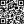
\includegraphics[width=0.8\textwidth]{qr_github_tofa.pdf}\par}
\vspace{0.2em}
{\small{\ml{$0$}{О книге и авторе}{About the book and the author}}\par}
}
\end{minipage}
\hspace{2em}
\begin{minipage}[t]{0.25\textwidth}
{\centering
{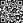
\includegraphics[width=0.8\textwidth]{qr_license_by40.pdf}\par}
\vspace{0.2em}
{\small{\ml{$0$}{Текст лицензии}{License full text}}\par}
}
\end{minipage}
\hfill}
% ----- QR CODES -----

}
% ----- INFO PAGE -----

% ----- EMPTY PAGE -----
\newpage\thispagestyle{plain}~
% ----- EMPTY PAGE -----

% ----- BACK COVER -----

\includepdf[pages={1}]{cover_back.pdf}
% ----- BACK COVER -----

\end{document}
